% ============================================================================
% LULU WRAP COVER - Single-page cover spread with bleed
% ============================================================================
% Draws everything directly (no pre-rendered PDFs) so background elements
% extend seamlessly into bleed areas.
% ============================================================================

\documentclass[10pt]{book}

% ==========================================================================
% LOAD PREAMBLE (packages, colors, tikz, boxes, styling, commands)
% ==========================================================================
\documentclass[11pt]{article}

% ============================================================================
% MODERN TYPOGRAPHY AND LAYOUT
% ============================================================================
\usepackage[margin=1.2in, top=1.3in, bottom=1.3in]{geometry}
\usepackage[utf8]{inputenc}
\usepackage[T1]{fontenc}

% Modern font: Libertinus (elegant, readable serif)
\usepackage{libertinus}
\usepackage{libertinust1math}

% Typography enhancements
\usepackage{microtype}
\usepackage{setspace}
\setstretch{1.15}

% Paragraph formatting
\usepackage{parskip}
\setlength{\parskip}{0.5em}
\setlength{\parindent}{0pt}

% Language and quotation support
\usepackage[english]{babel}
\usepackage{csquotes}

% ============================================================================
% MATHEMATICS AND SYMBOLS
% ============================================================================
\usepackage{amsmath}
\usepackage{amssymb}

% ============================================================================
% GRAPHICS AND FIGURES
% ============================================================================
\usepackage{graphicx}
\usepackage{float}

% ============================================================================
% COLOR SYSTEM - Educational Semantic Palette
% ============================================================================
\usepackage{xcolor}

% LAYER 1: PRIMITIVE COLOR PALETTE
\definecolor{slate-900}{RGB}{30,58,95}
\definecolor{slate-700}{RGB}{71,101,135}
\definecolor{slate-100}{RGB}{240,246,252}
\definecolor{green-900}{RGB}{46,125,50}
\definecolor{green-600}{RGB}{67,160,71}
\definecolor{green-100}{RGB}{232,245,233}
\definecolor{amber-900}{RGB}{230,124,0}
\definecolor{amber-600}{RGB}{251,140,0}
\definecolor{amber-100}{RGB}{255,243,224}
\definecolor{red-900}{RGB}{198,40,40}
\definecolor{red-600}{RGB}{229,57,53}
\definecolor{red-100}{RGB}{255,235,238}
\definecolor{teal-700}{RGB}{0,128,128}
\definecolor{teal-600}{RGB}{0,137,123}
\definecolor{teal-100}{RGB}{224,242,241}
\definecolor{indigo-700}{RGB}{63,81,181}
\definecolor{indigo-600}{RGB}{92,107,192}
\definecolor{indigo-100}{RGB}{232,234,246}
\definecolor{gray-900}{RGB}{30,32,34}
\definecolor{gray-800}{RGB}{52,58,64}
\definecolor{gray-700}{RGB}{73,80,87}
\definecolor{gray-600}{RGB}{95,100,105}
\definecolor{gray-500}{RGB}{134,142,150}
\definecolor{gray-400}{RGB}{173,181,189}
\definecolor{gray-300}{RGB}{210,215,220}
\definecolor{gray-200}{RGB}{233,236,239}
\definecolor{gray-100}{RGB}{247,248,250}
\definecolor{cream-100}{RGB}{252,250,246}

% LAYER 2: SEMANTIC COLOR MAPPINGS
\definecolor{definition-dark}{RGB}{30,58,95}
\definecolor{definition-base}{RGB}{71,101,135}
\definecolor{definition-light}{RGB}{240,246,252}
\definecolor{example-dark}{RGB}{46,125,50}
\definecolor{example-base}{RGB}{67,160,71}
\definecolor{example-light}{RGB}{232,245,233}
\definecolor{key-dark}{RGB}{230,124,0}
\definecolor{key-base}{RGB}{251,140,0}
\definecolor{key-light}{RGB}{255,243,224}
\definecolor{caution-dark}{RGB}{198,40,40}
\definecolor{caution-base}{RGB}{229,57,53}
\definecolor{caution-light}{RGB}{255,235,238}
\definecolor{note-dark}{RGB}{73,80,87}
\definecolor{note-base}{RGB}{134,142,150}
\definecolor{note-light}{RGB}{252,250,246}
\definecolor{theorem-dark}{RGB}{63,81,181}
\definecolor{theorem-base}{RGB}{92,107,192}
\definecolor{theorem-light}{RGB}{232,234,246}
\definecolor{practice-dark}{RGB}{0,128,128}
\definecolor{practice-base}{RGB}{0,137,123}
\definecolor{practice-light}{RGB}{224,242,241}

% LAYER 3: COMPONENT-SPECIFIC ALIASES
\definecolor{text-primary}{RGB}{30,32,34}
\definecolor{text-secondary}{RGB}{73,80,87}
\definecolor{text-muted}{RGB}{95,100,105}
\definecolor{bg-definition}{RGB}{240,246,252}
\definecolor{bg-example}{RGB}{232,245,233}
\definecolor{bg-key}{RGB}{255,243,224}
\definecolor{bg-caution}{RGB}{255,235,238}
\definecolor{bg-note}{RGB}{252,250,246}
\definecolor{bg-theorem}{RGB}{232,234,246}
\definecolor{bg-practice}{RGB}{224,242,241}
\definecolor{bg-neutral}{RGB}{247,248,250}
\definecolor{border-definition}{RGB}{71,101,135}
\definecolor{border-example}{RGB}{67,160,71}
\definecolor{border-key}{RGB}{251,140,0}
\definecolor{border-caution}{RGB}{229,57,53}
\definecolor{border-note}{RGB}{210,215,220}
\definecolor{border-theorem}{RGB}{92,107,192}
\definecolor{border-practice}{RGB}{0,137,123}
\definecolor{border-neutral}{RGB}{210,215,220}
\definecolor{primary}{RGB}{30,58,95}
\definecolor{primary-light}{RGB}{71,101,135}
\definecolor{accent}{RGB}{251,140,0}

% ============================================================================
% TABLES - Modern styling
% ============================================================================
\usepackage{booktabs}
\usepackage{longtable}
\usepackage{array}
\usepackage{multirow}
\usepackage{tabularx}
\usepackage{colortbl}
\usepackage{pdflscape}
\renewcommand{\arraystretch}{1.3}

% ============================================================================
% BOXES AND VISUAL ELEMENTS
% ============================================================================
\usepackage{tcolorbox}
\tcbuselibrary{breakable,skins,theorems,listings}

\usepackage{listings}
\lstset{
  basicstyle=\small\ttfamily\color{gray-900},
  breaklines=true,
  breakatwhitespace=false,
  columns=flexible,
  keepspaces=true,
  showstringspaces=false,
  tabsize=2,
  xleftmargin=0pt,
  framexleftmargin=0pt,
  keywordstyle=\color{slate-700}\bfseries,
  stringstyle=\color{green-900},
  commentstyle=\color{gray-600}\itshape,
  emphstyle=\color{amber-900},
}

\tcbset{
  importance/.is choice,
  importance/high/.style={boxrule=2pt,drop shadow={shadow xshift=1pt, shadow yshift=-1pt, opacity=0.12},top=10pt,bottom=10pt,left=12pt,right=12pt},
  importance/medium/.style={},
  importance/low/.style={boxrule=0.8pt,drop shadow={opacity=0},opacityback=0.92,opacityframe=0.6,boxed title style={opacityback=0.85},top=6pt,bottom=6pt,left=8pt,right=8pt},
  importance/.default=medium
}

\newtcolorbox{definitionbox}[1][]{enhanced,colback=bg-definition,colframe=border-definition,fonttitle=\bfseries\large,coltitle=white,boxrule=1.5pt,arc=3pt,left=10pt,right=10pt,top=10pt,bottom=10pt,breakable,drop shadow={shadow xshift=1pt, shadow yshift=-1pt, opacity=0.08},attach boxed title to top left={yshift=-2mm, xshift=4mm},boxed title style={colback=definition-dark,colframe=definition-dark,arc=2pt,boxrule=0pt},#1}

\newtcolorbox{highlightbox}[1][]{enhanced,colback=bg-note,colframe=border-note,fonttitle=\bfseries,coltitle=note-dark,boxrule=1pt,arc=2.5pt,left=10pt,right=10pt,top=8pt,bottom=8pt,breakable,drop shadow={shadow xshift=0.5pt, shadow yshift=-0.5pt, opacity=0.05},#1}

\newtcolorbox{keybox}[1][]{enhanced,colback=bg-key,colframe=key-base,fonttitle=\bfseries\large,coltitle=white,boxrule=2pt,arc=3pt,left=12pt,right=12pt,top=10pt,bottom=10pt,breakable,drop shadow={shadow xshift=1pt, shadow yshift=-1pt, opacity=0.1},borderline west={3pt}{0pt}{key-base},attach boxed title to top left={yshift=-2mm, xshift=4mm},boxed title style={colback=key-base,colframe=key-base,arc=2pt,boxrule=0pt},#1}

\newtcolorbox{questionbox}[1][]{enhanced,colback=gray-100,colframe=gray-600,fonttitle=\bfseries,coltitle=white,boxrule=1.5pt,arc=2pt,left=10pt,right=10pt,top=8pt,bottom=8pt,breakable,borderline west={4pt}{0pt}{slate-700},attach boxed title to top left={yshift=-2mm, xshift=4mm},boxed title style={colback=slate-700,colframe=slate-700,arc=2pt,boxrule=0pt},#1}

\newtcolorbox{theorembox}[1][]{enhanced,colback=bg-theorem,colframe=border-theorem,fonttitle=\bfseries\large,coltitle=white,boxrule=1.5pt,arc=3pt,left=12pt,right=12pt,top=10pt,bottom=10pt,breakable,drop shadow={shadow xshift=1pt, shadow yshift=-1pt, opacity=0.08},attach boxed title to top left={yshift=-2mm, xshift=4mm},boxed title style={colback=theorem-dark,colframe=theorem-dark,arc=2pt,boxrule=0pt},#1}

\newtcblisting{listingbox}[1][]{enhanced,colback=gray-100,colframe=gray-400,fonttitle=\bfseries\sffamily,coltitle=gray-800,boxrule=1pt,arc=2pt,left=8pt,right=8pt,top=6pt,bottom=6pt,breakable,listing only,listing options={basicstyle=\small\ttfamily\color{gray-900},breaklines=true,columns=flexible,keepspaces=true},attach boxed title to top left={yshift=-2mm, xshift=4mm},boxed title style={colback=gray-500,colframe=gray-500,arc=2pt,boxrule=0pt},#1}

% ============================================================================
% LISTS
% ============================================================================
\usepackage{enumitem}
\setlist{itemsep=0.4em,parsep=0.2em,topsep=0.5em,leftmargin=1.5em}

\newlist{evallist}{enumerate}{1}
\setlist[evallist]{label=\textbf{Q\arabic*.},leftmargin=2em,itemsep=0.5em,labelsep=0.5em}

% ============================================================================
% TIKZ
% ============================================================================
\usepackage{tikz}
\usetikzlibrary{positioning,arrows.meta,shapes.geometric,shapes.misc,calc,decorations.pathreplacing,backgrounds,fit,shadows.blur}
\tikzset{every node/.style={font=\normalfont},every text node part/.style={font=\normalfont}}

% ============================================================================
% SECTION STYLING
% ============================================================================
\usepackage{titlesec}
\usepackage{titletoc}

\titleformat{\section}{\Large\bfseries\color{primary}}{\thesection}{1em}{}[\vspace{0.3em}{\color{primary}\titlerule[1.5pt]}\vspace{0.5em}]
\titleformat{\subsection}{\large\bfseries\color{primary}}{\thesubsection}{1em}{}[\vspace{-0.3em}]
\titleformat{\subsubsection}{\normalsize\bfseries\color{text-secondary}}{\thesubsubsection}{1em}{}
\titleformat{\paragraph}[runin]{\normalsize\bfseries\color{primary}}{}{0em}{}[.]
\titlespacing*{\paragraph}{0pt}{1em}{0.5em}

% ============================================================================
% TABLE OF CONTENTS
% ============================================================================
\renewcommand{\contentsname}{{\color{primary}\Large\bfseries Contents}}
\titlecontents{section}[1.5em]{\vspace{0.5em}\bfseries}{\color{primary}\contentslabel{1.5em}}{}{\titlerule*[0.75pc]{.}\contentspage}
\titlecontents{subsection}[3.8em]{\vspace{0.2em}}{\contentslabel{2.3em}}{}{\titlerule*[0.75pc]{.}\contentspage}

% ============================================================================
% CAPTIONS
% ============================================================================
\usepackage[font={small},labelfont={bf,color=primary},format=plain,justification=justified,skip=8pt]{caption}

% ============================================================================
% HYPERLINKS
% ============================================================================
\usepackage{hyperref}
\hypersetup{
  colorlinks=true,
  linkcolor=primary,
  citecolor=accent,
  urlcolor=primary,
  bookmarksnumbered=true,
  pdfborder={0 0 0},
  pdftitle={Foundations: Conversations and Reasoning},
  pdfauthor={Michael J Bommarito II, Daniel Martin Katz, Jillian Bommarito},
  pdfsubject={LLM Conversations, Reasoning Patterns, Chain-of-Thought, ReAct},
  pdfkeywords={conversational AI, chain-of-thought, ReAct, reasoning, context management, prompt engineering}
}

\usepackage{cleveref}
\crefname{section}{Section}{Sections}
\crefname{figure}{Figure}{Figures}
\crefname{table}{Table}{Tables}

% ============================================================================
% BIBLIOGRAPHY
% ============================================================================
\usepackage[backend=biber,style=authoryear,maxcitenames=2,maxbibnames=99,uniquename=false,uniquelist=false,sorting=nyt,dashed=false]{biblatex}
\DeclareFieldFormat{citetitle}{\mkbibquote{#1}}
\DeclareFieldFormat[article]{citetitle}{#1}
\DeclareFieldFormat[inproceedings]{citetitle}{#1}
\DeclareFieldFormat[book]{citetitle}{\mkbibemph{#1}}
\DeclareFieldFormat[techreport]{citetitle}{#1}
\DeclareFieldFormat[misc]{citetitle}{#1}
\addbibresource{bib/refs.bib}

% ============================================================================
% CUSTOM COMMANDS
% ============================================================================
\newcommand{\keyterm}[1]{\textbf{\color{primary}#1}}
\newcommand{\levelone}[1]{\textbf{#1}}
\newcommand{\leveltwo}[1]{\textbf{#1}}
\newcommand{\levelthree}[1]{\textbf{#1}}

% ============================================================================
% TITLE AND METADATA
% ============================================================================
\title{
  \vspace{-0.5em}
  {\Huge\bfseries\color{primary} Foundations}\\[0.6em]
  {\LARGE\color{primary} Conversations and Reasoning}\\[0.4em]
  {\large\itshape\color{text-secondary} Chat Mechanics, Memory, and Reasoning Patterns}
  \vspace{0.5em}
}

\author{
  \vspace{-0.5em}
  {\large\color{text-muted}
    Michael J Bommarito II \enspace $\cdot$ \enspace
    Daniel Martin Katz \enspace $\cdot$ \enspace
    Jillian Bommarito
  }
  \vspace{-0.5em}
}

\date{{\normalsize\color{text-muted}\today}}

% ============================================================================
% DOCUMENT START
% ============================================================================
\begin{document}

\maketitle

% Decorative rule after title block
\vspace{-1em}
\noindent{\color{border-neutral}\rule{\textwidth}{0.5pt}}
\vspace{1.0em}

% Draft notice
\begin{center}
  \begin{tcolorbox}[
      enhanced,
      width=0.80\textwidth,
      colback=bg-note,
      colframe=border-note,
      fonttitle=\bfseries\large\color{note-dark},
      boxrule=1.5pt,
      arc=4pt,
      left=16pt,
      right=16pt,
      top=12pt,
      bottom=12pt,
      breakable,
      drop shadow={shadow xshift=1pt, shadow yshift=-1pt, opacity=0.08},
      borderline west={4pt}{0pt}{note-dark}
    ]

    \begin{center}
      {\large\bfseries\color{note-dark} Working Draft Chapter} \\[0.2em]
      {\small\color{text-muted} Version 0.1}
    \end{center}

    \vspace{0.25em}

    {\small
      This chapter is from the textbook \textit{Artificial Intelligence for Law and Finance}, currently under development. It covers the transition from single-shot completions to multi-turn conversations, context management strategies, and the reasoning patterns that enable complex problem-solving.

      \vspace{0.5em}

      The most current copy of the project is available at:\\
      \url{https://github.com/mjbommar/ai-law-finance-book/}
    }

  \end{tcolorbox}
\end{center}

\pagebreak

% Table of contents
\tableofcontents

\pagebreak

% ============================================================================
% MAIN CONTENT
% ============================================================================
% =============================================================================
% How to Read — LLM Primer & Mechanics
% Purpose: Audience paths; scope and outcomes; reading strategies
% Label prefix: sec:llm1-howtoread
% =============================================================================

\section*{How to Read This Chapter}
\addcontentsline{toc}{section}{How to Read This Chapter}

This chapter provides a comprehensive primer on the mechanics of Large Language Models (LLMs) for legal and financial professionals. Unlike user guides focused on specific tools, this chapter offers structural analysis of the technology itself---the foundational understanding you need to reason about model behavior from first principles.

\paragraph{Target Audience.} This chapter is designed for practitioners who must understand \emph{how} LLMs work, not just \emph{that} they work:

\begin{itemize}
  \item \textbf{Legal professionals} evaluating AI tools for document review, research, or drafting
  \item \textbf{Financial analysts and risk managers} deploying models for reporting, analysis, or client communication
  \item \textbf{Compliance officers} designing validation frameworks and governance controls
  \item \textbf{Technology leaders} architecting enterprise AI systems in regulated environments
  \item \textbf{Researchers and policy analysts} studying the intersection of AI, law, and finance
\end{itemize}

\begin{keybox}[title={Key Objectives}]
By the end of this chapter, you will be able to:
\begin{enumerate}
  \item \textbf{Understand the architecture}: Know why the Transformer succeeded where predecessors failed, and how this enables processing of long legal and financial documents.
  \item \textbf{Master the mechanics}: Grasp how tokenization, context windows, and sampling parameters directly affect output quality, cost, and reliability.
  \item \textbf{Reason about embeddings}: Understand how text becomes vectors, enabling semantic search that powers retrieval-augmented generation.
  \item \textbf{Anticipate failure}: Recognize intrinsic limitations---hallucinations, stochasticity, recency gaps---to build defensible guardrails.
  \item \textbf{Apply practical defaults}: Know which parameter settings are appropriate for regulated outputs versus creative exploration.
\end{enumerate}
\end{keybox}

\subsection*{Reading Paths by Role}

Different readers will benefit from different emphases. We suggest the following paths:

\paragraph{For the Strategic Leader (30 minutes).} Focus on \Cref{sec:llm1-history} (Conceptual Primer and Brief History) and \Cref{sec:llm1-fail} (Common Failure Modes). These sections outline the trajectory of AI capabilities defined by scaling laws and the operational risks---such as hallucination and data leakage---that define the liability profile of LLM deployment. Skim the technical sections to understand the vocabulary your teams will use.

\paragraph{For the AI Engineer and Architect (2--3 hours).} Read all sections thoroughly. \Cref{sec:llm1-tokens} (Tokens and Tokenizers), \Cref{sec:llm1-sampling} (Sampling and Decoding), and \Cref{sec:llm1-embeddings} (Representations and Embeddings) contain operational parameters that directly influence system performance, latency, and cost. Pay special attention to the discussion of constrained decoding and hybrid search architectures.

\paragraph{For the Risk and Compliance Officer (1--2 hours).} \Cref{sec:llm1-fail} (Failure Modes) provides the taxonomy of risks required for validation frameworks. Review governance considerations in \Cref{sec:llm1-history} regarding training data provenance and regulatory requirements (EU AI Act, OWASP Top 10 for LLMs). The practical defaults in \Cref{sec:llm1-sampling} will help you specify requirements for vendor evaluations.

\paragraph{For the Time-Constrained Reader (15 minutes).} If you have limited time, read this section's Key Objectives box, then skim:
\begin{enumerate}
  \item The ``Plain-English Summary'' boxes throughout
  \item \Cref{sec:llm1-history} through the first two subsections (through Scaling Laws)
  \item \Cref{sec:llm1-tokens} focusing on ``Token Economics'' and practical context constraints
  \item The ``Watch Outs'' cautionbox in \Cref{sec:llm1-fail}
\end{enumerate}

\subsection*{Relationship to Other Chapters}

This chapter provides foundational vocabulary and mental models that subsequent chapters build upon:

\begin{itemize}
  \item \textbf{Chapter 2 (Providing Context)} establishes grounding through in-context learning and retrieval-augmented generation. The discussion of embeddings and hybrid search here provides the conceptual foundation for connecting models to authoritative sources.

  \item \textbf{Chapter 3 (Reasoning and Conversations)} adds multi-turn dialogue, chain-of-thought prompting, and reasoning strategies. Understanding tokens and context windows here is prerequisite for managing conversation state there.

  \item \textbf{Agentic Systems} (covered in our companion volume, \textit{Agentic AI in Law and Finance}) assume familiarity with all concepts in this chapter. Tool-calling agents require structured outputs (constrained decoding), and agent loops must handle the stochastic nature of LLM outputs.

  \item \textbf{Governance Frameworks} build on the failure mode taxonomy here to specify validation frameworks, monitoring systems, and compliance controls.
\end{itemize}

\begin{highlightbox}[title={A Note on Technical Depth}]
This chapter deliberately operates at the conceptual level. We explain \emph{what} attention mechanisms do and \emph{why} they matter, but we do not derive the mathematics. Readers seeking mathematical foundations should consult the primary sources cited in \Cref{sec:llm1-further}. Our goal is practical understanding: you should finish this chapter able to reason about why a particular configuration might produce unreliable outputs, even without being able to implement a Transformer from scratch.
\end{highlightbox}

\begin{highlightbox}[title={Visual Cues (Boxes)}]
Throughout the chapter, colored boxes signal intent:
\begin{itemize}
  \item \textbf{Key takeaways (\texttt{keybox}):} objectives, practical defaults, and decision-relevant summaries
  \item \textbf{Notes (\texttt{highlightbox}):} plain-English summaries and contextual intuition
  \item \textbf{Optional technical detail (\texttt{technicalbox}):} deeper mechanics (hardware, arrays, algorithms) that you can safely skip on a first read
  \item \textbf{Warnings (\texttt{cautionbox}):} red ``watch outs'' for risk, failure modes, and compliance pitfalls
  \item \textbf{Code/examples (\texttt{listingbox}):} reproducible snippets and technical artifacts (when included)
\end{itemize}
\end{highlightbox}

\subsection*{Terminology Conventions}

Throughout this chapter, we use the following terminology consistently:

\begin{itemize}
  \item \keyterm{LLM} (Large Language Model): A neural network trained on massive text corpora to predict and generate text. Examples include GPT-4, Claude, Llama, and Gemini.

  \item \keyterm{Token}: The atomic unit of text processing---typically a subword piece, punctuation mark, or character sequence.

  \item \keyterm{Context window}: The maximum sequence length (input + output tokens) a model can process in a single pass.

  \item \keyterm{Completion}: The text generated by the model in response to a prompt.

  \item \keyterm{Hallucination}: Model-generated content that is factually incorrect, ungrounded, or fabricated.

  \item \keyterm{Embedding}: A high-dimensional vector representation of text that captures semantic meaning.

  \item \keyterm{Sampling}: The process by which a model selects the next token from its predicted probability distribution.
\end{itemize}

These terms will be defined more precisely as we encounter them. For now, this glossary provides orientation for the material ahead.

% =============================================================================
% Introduction — How Do I Ground and Reason?
% Purpose: Scope, motivation, and chapter roadmap with grounding-first framing
% Label: sec:llmB-intro
% =============================================================================

\section{Introduction: Why Grounding Comes First}
\label{sec:llmB-intro}

An architect would never design a building without first surveying the site. The soil composition, property boundaries, existing utilities, and zoning constraints must be understood before a single line is drawn. Similarly, a litigator would never draft a brief without first researching the applicable law. The governing statutes, binding precedent, and controlling regulations must be identified before constructing any argument. In both cases, the professional's reasoning ability is necessary but insufficient. Without access to the relevant facts, even the most sophisticated analysis proceeds in a vacuum.

Large Language Models face exactly the same constraint. A model can reason impressively about legal doctrines and financial concepts, but without mechanisms to access current case law, live market data, client documents, or regulatory filings, it cannot deliver reliable professional work. This chapter addresses how to transform a powerful but potentially ungrounded reasoning engine into a system that reasons \emph{from} authoritative sources rather than about them from memory alone.

\subsection{From ``Prevent Hallucination'' to ``Enable Capability''}

The conventional framing of retrieval-augmented generation (RAG) positions it as a defensive measure: models hallucinate, so we give them documents to reduce errors. This framing, while not wrong, misses the deeper point. Grounding is not primarily about preventing failure; it is about \emph{enabling capability}.

Consider the difference between these two instructions to an LLM:

\begin{quote}
\textit{``Analyze whether the client's termination of the software license agreement was proper.''}
\end{quote}

\begin{quote}
\textit{``Analyze whether the client's termination of the software license agreement was proper, based on the attached agreement and the following Delaware case law on software licensing...''}
\end{quote}

The first instruction asks the model to reason from general knowledge. The second provides the specific materials needed to perform actual legal analysis. The difference is not merely that the second is safer; it is that the second is \emph{capable} of producing professional work while the first is not, regardless of the model's sophistication.

\begin{keybox}[title={The Grounding Principle}]
Grounding is not a fix for hallucination---it is an architectural necessity for professional reasoning. An ungrounded model can discuss legal concepts; a grounded model can analyze specific legal situations. The distinction is fundamental.
\end{keybox}

This reframing has practical consequences. If grounding is merely a safety mechanism, you might add it late in development after building your reasoning pipelines. If grounding is a capability enabler, you design it into the architecture from the beginning. This chapter takes the latter approach.

\subsection{The Dual Challenge Revisited}

Chapter~1 introduced the mechanics of LLMs: how tokens become probabilities, how sampling produces text, and how failure modes emerge. With those foundations established, we now face the practical challenge of building systems that can assist with professional work. This requires addressing two interconnected problems:

\begin{definitionbox}[title={Challenge 1: Grounded Context}]
How do we provide the model with the specific information it needs to reason about a particular matter? This includes retrieving relevant documents, maintaining conversation state, and ensuring the model has access to authoritative sources rather than relying on general knowledge.
\end{definitionbox}

\begin{definitionbox}[title={Challenge 2: Structured Reasoning}]
How do we elicit systematic reasoning over that grounded context? Standard ``zero-shot'' prompting often fails on complex tasks because the model attempts to map input directly to output in a single forward pass, relying on surface-level statistical correlations rather than step-by-step analysis \parencite{wei2022cot}.
\end{definitionbox}

These challenges are deeply interrelated. Effective reasoning requires relevant context, while determining what context is relevant often requires reasoning about the task. The techniques we introduce---from in-context learning to retrieval-augmented generation to chain-of-thought reasoning---address both challenges in an integrated framework.

Crucially, the order matters. We begin with grounding because reasoning without relevant context is speculation, no matter how sophisticated the reasoning patterns employed. A perfectly constructed chain-of-thought analysis based on hallucinated precedent is worse than useless in professional practice.

\subsection{Chapter Roadmap}

This chapter builds from foundations to practice, following the logical order in which these concepts support each other:

\paragraph{\Cref{sec:llmB-icl}: In-Context Learning.} We begin with the fundamental mechanism that makes grounding effective: the ability of LLMs to learn from information provided in their input, without any update to model weights. Understanding in-context learning explains why few-shot examples work, why RAG is effective, and why conversation history shapes model behavior.

\paragraph{\Cref{sec:llmB-rag}: Grounding via Retrieval.} With in-context learning established, we examine how to populate that context with relevant information. Retrieval-augmented generation (RAG) provides the model with authoritative sources---case law, regulations, financial data, client documents---rather than relying on parametric knowledge alone.

\paragraph{\Cref{sec:llmB-domain}: Professional Domain Requirements.} General-purpose retrieval is insufficient for regulated industries. Legal and financial applications require authority hierarchies (binding vs. persuasive precedent), jurisdictional filtering, temporal validity checking, and matter isolation to maintain confidentiality boundaries.

\paragraph{\Cref{sec:llmB2-synthesis}: Synthesis.} We integrate the concepts and prepare the transition to reasoning patterns covered in Chapter~3.

\subsection{A Note on Prerequisites}

This chapter assumes familiarity with the LLM mechanics from Chapter~1, particularly:

\begin{itemize}
  \item \keyterm{Context windows}: The maximum number of tokens the model can consider in a single inference call (\Cref{sec:llm1-tokens}).

  \item \keyterm{Embeddings}: Vector representations of text that capture semantic meaning (\Cref{sec:llm1-embeddings}).

  \item \keyterm{Sampling parameters}: How temperature and other settings affect generation behavior (\Cref{sec:llm1-sampling}).
\end{itemize}

If these concepts are unfamiliar, consider reviewing the relevant sections of Chapter~1 before proceeding. The techniques in this chapter build directly on those foundations.

\subsection{What This Chapter Does Not Cover}

While we introduce retrieval-augmented generation and professional domain requirements, this chapter focuses on providing context to models. Related topics are addressed elsewhere:

\begin{itemize}
  \item \textbf{Reasoning patterns} (chain-of-thought, self-consistency, ReAct) appear in Chapter~3, which builds on the grounded context established here.

  \item \textbf{Conversation state management} (multi-turn dialogue, memory strategies) is covered in Chapter~3.

  \item \textbf{Structured output enforcement} (JSON schemas, function calling, validation) is covered in Chapter~4.

  \item \textbf{Tool use} (function calling, API integration) appears in Chapter~5.

  \item \textbf{Multimodal inputs} (document images, tables, audio) are addressed in Chapter~6.

  \item \textbf{Evaluation and optimization} of retrieval and reasoning pipelines appear in Chapter~7.
\end{itemize}

With this roadmap established, we turn to the foundational concept that makes all grounding techniques effective: in-context learning.

% =============================================================================
% Conversational Models and State — Conversations & Reasoning
% Purpose: Roles, memory/state, chat mechanics, guardrails
% Label: sec:llmB-convo
% =============================================================================

\section{Conversational Models and State}
\label{sec:llmB-convo}

The distinction between a text-completion engine and a conversational agent lies entirely in the management of state. Since the underlying model weights are frozen and stateless, ``memory'' is purely a function of the input context. To maintain a conversation, the orchestration layer must recursively re-inject the history of the interaction into the model's context window with each new turn. This process, often termed \keyterm{context rehydration}, is the fundamental mechanic of conversational AI.

However, treating the context window as an infinite append-only log is computationally unsustainable and algorithmically flawed. Context windows have fixed limits---ranging from 4,096 tokens in older models to 128,000+ in newer iterations---and the attention mechanism itself has limitations that affect how well the model can access different parts of a long context.

In this section, we examine the architectural components of conversational state: the role-based prompt structure that defines who is speaking and what constraints apply, the memory strategies that maintain coherence across turns, and the safety mechanisms that bound model behavior.

\subsection{Role-Based Prompt Engineering}
\label{sec:llmB-roles}

Modern conversational architectures enforce a strict separation of concerns through \keyterm{role-based prompting}. This is not merely a formatting convention but a control mechanism that delineates the model's operational constraints from user inputs. The architecture recognizes three primary roles: the \textbf{System}, the \textbf{User}, and the \textbf{Assistant}.

\subsubsection{The System Role: The Immutable Constitution}
\label{sec:llmB-system-role}

The \keyterm{system prompt} (often designated with special control tokens in the model's vocabulary) serves as the immutable ``constitution'' of the agent. It establishes the behavioral baseline, tone, output format, and, crucially, the safety boundaries of the interaction \parencite{zheng2023personas}.

Unlike user prompts, which are dynamic, untrusted, and variable, the system prompt is intended to be static and privileged. In architectures like Llama 2, the input is structured to wrap user messages in specific tags while separating the system instruction, ensuring the attention heads distinguish between instructions to be followed and text to be processed \parencite{touvron2023llama2}. This structural separation is vital for defense against ``jailbreaking'' or ``prompt injection'' attacks, where a user attempts to override the model's safety protocols by mimicking authoritative instructions.

\paragraph{Signpost to Chapter~1.} Prompt injection is not only a conversational concern but also a core LLM failure mode with security implications. Chapter~1 provides a detailed taxonomy of prompt injection and defense-in-depth mitigations.

\begin{keybox}[title={Effective System Prompt Design}]
An effective system prompt should include:
\begin{enumerate}
  \item \textbf{Identity and role}: Define who the assistant is and its primary purpose
  \item \textbf{Behavioral constraints}: Specify what the assistant should and should not do
  \item \textbf{Output format}: Establish expected structure for responses (when applicable)
  \item \textbf{Knowledge boundaries}: Define what the assistant knows and when to acknowledge uncertainty
  \item \textbf{Escalation criteria}: Specify when to refuse, ask for clarification, or defer to human judgment
\end{enumerate}
\end{keybox}

\paragraph{Example: Legal Research Assistant.} Consider a system prompt for a legal research assistant:

\begin{quote}
\texttt{You are a legal research assistant specializing in U.S. federal law. You help attorneys find relevant case law, statutes, and regulations. You always cite specific sources with proper legal citations. You acknowledge when a question falls outside your knowledge or when case law may have evolved since your training. You never provide legal advice or make predictions about case outcomes. When asked about jurisdiction-specific rules, you note that local practice may vary and recommend verifying with current local sources.}
\end{quote}

This prompt establishes identity (legal research assistant), scope (U.S. federal law), expected behavior (cite sources, acknowledge limitations), prohibitions (no legal advice or predictions), and appropriate hedging (verify with local sources).

\paragraph{Instruction Drift and Mitigation.} However, the efficacy of the system prompt is not absolute. A phenomenon known as \keyterm{instruction drift} or \keyterm{context dilution} can occur as the conversation lengthens. As the distance between the initial system prompt and the current generation increases, the model's adherence to the initial constraints can degrade, primarily due to the ``recency bias'' inherent in the attention mechanism \parencite{liu2024lostmiddle}.

To combat this, advanced prompting strategies involve:
\begin{itemize}
  \item \textbf{Repeating critical constraints}: Restate key rules near the end of the prompt, immediately before the generation trigger
  \item \textbf{Periodic reinforcement}: Insert reminder statements in long conversations (e.g., ``Remember, you should not provide legal advice'')
  \item \textbf{Sentinel phrases}: Use specific phrases that trigger compliance checks (though this requires custom orchestration logic)
\end{itemize}

\subsubsection{The User and Assistant Roles: Managing the Dialogue Loop}

The \textbf{user role} represents external input---the queries, commands, and information provided by the human interacting with the system. The \textbf{assistant role} captures the model's generated outputs. To maintain state, the application must append each user query and assistant response to a growing list of messages. This list is serialized into a single prompt string (or a structured token sequence) at every turn.

\begin{definitionbox}[title={The Dialogue Loop}]
A typical multi-turn conversation follows this pattern:
\begin{enumerate}
  \item Receive user input
  \item Construct prompt: \texttt{[System] + [History] + [User Input]}
  \item Call model, generate response
  \item Append \texttt{[User Input, Assistant Response]} to history
  \item Return response to user
  \item Repeat from step 1
\end{enumerate}
\end{definitionbox}

The integrity of this dialogue loop is maintained through strict formatting. For instance, Llama 2 uses a specific syntax where the system prompt and user prompt are enclosed in special tags, but the model's response is left outside, creating a clear demarcation in the token stream. This formatting guides the model's stop-token prediction; without it, the model might hallucinate the user's next response rather than stopping after its own turn.

\paragraph{Practical Implications.} When constructing prompts:
\begin{itemize}
  \item \textbf{Be explicit}: Don't assume the model remembers what ``it'' refers to from five turns back unless you've managed context accordingly
  \item \textbf{Reference context}: If a question relates to something said much earlier, remind the model: ``Based on our discussion about X earlier, ...''
  \item \textbf{Use retrieval}: For long conversations, retrieve and inject the exact relevant snippet rather than relying on raw history
\end{itemize}

\subsection{Memory Strategies: Maintaining Context in Dialogues}
\label{sec:llmB-memory}

One of the biggest challenges in multi-turn conversations is how the model ``remembers'' earlier parts of the dialogue. Given the finite nature of the context window, managing conversation history is fundamentally a \emph{resource allocation problem}. As the conversation exceeds the window size, the system must make active decisions about what to retain and what to discard.

\subsubsection{The ``Lost in the Middle'' Phenomenon}

A critical insight in context management is that LLMs do not access all parts of their context window with equal acuity. Extensive empirical analysis reveals a distinct U-shaped performance curve regarding information retrieval \parencite{liu2024lostmiddle}. Models excel at retrieving information located at the very beginning (primacy effect) and the very end (recency effect) of the input context. Information buried in the middle of a long sequence is significantly more likely to be ignored, hallucinated, or incorrectly associated.

\begin{keybox}[title={The U-Shaped Retrieval Curve}]
When retrieving facts from context:
\begin{itemize}
  \item \textbf{Beginning of context}: High retrieval accuracy (primacy effect)
  \item \textbf{Middle of context}: Significantly degraded accuracy
  \item \textbf{End of context}: High retrieval accuracy (recency effect)
\end{itemize}
This phenomenon is likely an emergent property of training data structure, where introductions and conclusions contain concentrated semantic signal.
\end{keybox}

\Cref{fig:llmB-lost-middle} illustrates this U-shaped retrieval curve, showing how information placement affects model attention.

\begin{figure}[htbp]
  \centering
  \resizebox{0.95\textwidth}{!}{% =============================================================================
% Figure: Lost in the Middle
% Shows the U-shaped attention curve
% =============================================================================

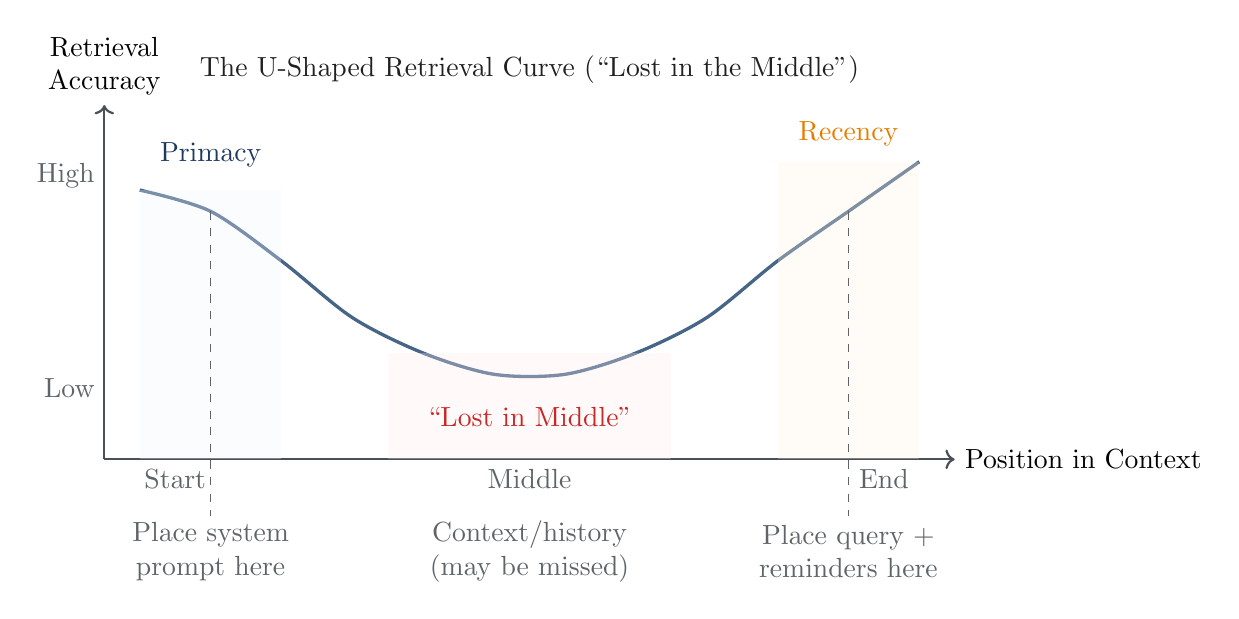
\begin{tikzpicture}[
  scale=0.9,
  label/.style={
    font=\footnotesize,
    text=text-muted
  }
]

% Axes
\draw[->, thick, draw=text-secondary] (0,0) -- (12,0) node[right, font=\small] {Position in Context};
\draw[->, thick, draw=text-secondary] (0,0) -- (0,5) node[above, font=\small, align=center] {Retrieval\\Accuracy};

% X-axis labels
\node[label, below] at (1,0) {Start};
\node[label, below] at (6,0) {Middle};
\node[label, below] at (11,0) {End};

% Y-axis labels
\node[label, left] at (0,1) {Low};
\node[label, left] at (0,4) {High};

% U-shaped curve
\draw[very thick, draw=definition-base, smooth] plot coordinates {
  (0.5, 3.8)
  (1.5, 3.5)
  (2.5, 2.8)
  (3.5, 2.0)
  (4.5, 1.5)
  (5.5, 1.2)
  (6.5, 1.2)
  (7.5, 1.5)
  (8.5, 2.0)
  (9.5, 2.8)
  (10.5, 3.5)
  (11.5, 4.2)
};

% Shaded regions
\fill[definition-light, opacity=0.3] (0.5,0) rectangle (2.5,3.8);
\fill[caution-light, opacity=0.3] (4,0) rectangle (8,1.5);
\fill[key-light, opacity=0.3] (9.5,0) rectangle (11.5,4.2);

% Annotations
\node[font=\footnotesize\bfseries, text=definition-dark] at (1.5, 4.3) {Primacy};
\node[font=\footnotesize\bfseries, text=caution-dark] at (6, 0.6) {``Lost in Middle''};
\node[font=\footnotesize\bfseries, text=key-dark] at (10.5, 4.6) {Recency};

% Practical implications
\draw[dashed, draw=text-muted] (1.5, 3.5) -- (1.5, -0.8);
\draw[dashed, draw=text-muted] (10.5, 3.5) -- (10.5, -0.8);
\node[label, align=center] at (1.5, -1.3) {Place system\\prompt here};
\node[label, align=center] at (10.5, -1.3) {Place query +\\reminders here};
\node[label, align=center] at (6, -1.3) {Context/history\\(may be missed)};

% Title
\node[font=\bfseries\small, text=text-primary] at (6, 5.5) {The U-Shaped Retrieval Curve (``Lost in the Middle'')};

\end{tikzpicture}
}
  \caption{The ``Lost in the Middle'' phenomenon: LLMs exhibit a U-shaped retrieval curve, with high accuracy at the beginning (primacy) and end (recency) of context, but degraded performance in the middle. This has profound implications for prompt construction.}
  \label{fig:llmB-lost-middle}
\end{figure}

The implications for conversation design are profound. Simply filling the context window with relevant documents or history does not guarantee retrieval. To mitigate this:
\begin{itemize}
  \item \textbf{Prompt re-ranking}: Relocate the most critical information to the beginning or immediate end of the prompt
  \item \textbf{Chunking with overlap}: Break long content into chunks with semantic boundaries, ensuring critical information appears at chunk boundaries
  \item \textbf{Explicit signaling}: Use formatting (headers, bullet points) to make critical information more salient
\end{itemize}

\subsubsection{Sliding Windows}

The simplest memory management strategy retains only the most recent $N$ tokens or turns. This \keyterm{sliding window} approach:

\begin{itemize}
  \item \textbf{Advantages}: Computationally simple, ensures high recency, predictable token usage
  \item \textbf{Disadvantages}: Induces ``catastrophic forgetting'' of earlier context; critical constraints or facts established early are lost once they slide out of the window
\end{itemize}

\paragraph{When to Use.} Sliding windows are appropriate when:
\begin{itemize}
  \item The conversation is inherently short-term (e.g., simple Q\&A)
  \item Recent context is far more relevant than historical context
  \item You have other mechanisms (like system prompts) to maintain critical constraints
\end{itemize}

\subsubsection{Recursive Summarization}

A more sophisticated approach employs the LLM itself to periodically compress older turns into a concise narrative summary \parencite{wang2024recursivesummarizing}. For example, after 10 turns, the model might summarize the dialogue as ``User asked about Python lists; Assistant explained syntax and provided examples.'' This summary is then prepended to the active context, replacing the raw tokens.

\begin{itemize}
  \item \textbf{Advantages}: Preserves the semantic ``gist'' of the conversation, frees up token space for new content
  \item \textbf{Disadvantages}: Lossy compression; specific details (e.g., a phone number, a specific code snippet, exact client instructions) may be smoothed over
\end{itemize}

\paragraph{Implementation Considerations.}
\begin{itemize}
  \item \textbf{Summarization frequency}: Every $N$ turns, or when the history exceeds a token threshold
  \item \textbf{Preservation of critical facts}: Maintain a separate ``pinned facts'' section for information that must never be summarized away
  \item \textbf{Hierarchical summarization}: For very long conversations, summarize summaries recursively
\end{itemize}

\begin{highlightbox}[title={Legal Application: Client Interview Memory}]
In a legal intake scenario, you might configure memory as follows:
\begin{itemize}
  \item \textbf{Pinned facts}: Client name, case type, jurisdiction, key dates (never summarized)
  \item \textbf{Active window}: Last 5 turns (full detail)
  \item \textbf{Summarized history}: Earlier turns compressed to key facts and decisions
\end{itemize}
This ensures the attorney always sees critical identifying information while maintaining context efficiency.
\end{highlightbox}

\subsubsection{Vector-Enhanced Memory (Long-Term Retrieval)}

For indefinite memory, systems employ external \keyterm{vector stores}. Conversation turns are embedded into vectors and stored in a database (using indices like HNSW or FAISS). When a new user query arrives, the system retrieves semantically relevant past interactions---regardless of temporal distance---and injects them into the current context \parencite{zhang2024memory}.

\paragraph{Signpost to Chapter~1.} Chapter~1 provides the primary treatment of embeddings, similarity metrics, and hybrid retrieval. This section focuses on how retrieval is used to implement conversational memory.

\begin{itemize}
  \item \textbf{Advantages}: Approximates human episodic memory; can retrieve relevant context from arbitrarily long histories; enables cross-session memory
  \item \textbf{Disadvantages}: Introduces latency; requires embedding model and vector database infrastructure; can surface conflicting memories if user preferences changed
\end{itemize}

\paragraph{Hybrid Approaches.} In practice, the most robust systems combine strategies:
\begin{enumerate}
  \item \textbf{System prompt}: Immutable constraints and identity
  \item \textbf{Pinned facts}: Critical session-specific information that must persist
  \item \textbf{Retrieved context}: Semantically relevant prior exchanges or documents
  \item \textbf{Summarized history}: Compressed earlier conversation
  \item \textbf{Active window}: Recent turns in full detail
  \item \textbf{Current query}: The user's latest input
\end{enumerate}

This layered approach maximizes the utility of the limited context window while maintaining coherence.

\begin{highlightbox}[title={Bridge to Agentic Systems}]
These memory patterns become architectural decisions in agentic systems. Our companion volume, \textit{Agentic AI in Law and Finance}, examines Memory as one of the core design questions for agents---addressing how agents maintain state across iterations and sessions.
\end{highlightbox}

\subsection{Context Management and Instruction Placement}
\label{sec:llmB-context-mgmt}

Given the ``Lost in the Middle'' phenomenon, where you place information in the prompt matters as much as what information you include.

\subsubsection{Token Budgeting}

Before constructing any prompt, establish a token budget:

\begin{enumerate}
  \item \textbf{Determine total available tokens}: Model context limit (e.g., 128K)
  \item \textbf{Reserve for output}: Allocate space for the expected response (e.g., 2K--4K tokens for detailed answers)
  \item \textbf{Allocate to components}:
  \begin{itemize}
    \item System prompt: 500--1,000 tokens
    \item Few-shot examples (if used): 1,000--3,000 tokens
    \item Retrieved context (RAG): Variable, often 2,000--10,000 tokens
    \item Conversation history: Remainder
    \item Current query: Usually small
    \item Final instructions/reminders: 100--200 tokens
  \end{itemize}
\end{enumerate}

\subsubsection{Optimal Instruction Placement}

Because LLMs weight recent tokens more heavily, the \emph{end} of the prompt (just before generation begins) is prime real estate. Place critical instructions there:

\begin{keybox}[title={The ``Sandwich'' Pattern}]
Structure your prompt as:
\begin{enumerate}
  \item \textbf{Beginning}: System prompt with core identity and constraints
  \item \textbf{Middle}: Context, history, retrieved documents
  \item \textbf{End}: Current query + \emph{reinforcement of critical constraints}
\end{enumerate}
The final reinforcement ensures that key rules (output format, prohibited actions, required disclaimers) are fresh in the model's ``attention'' when it begins generating.
\end{keybox}

\Cref{fig:llmB-context-assembly} illustrates the recommended ordering for prompt construction, showing how each layer builds on the previous.

\begin{figure}[htbp]
  \centering
  \resizebox{0.85\textwidth}{!}{% =============================================================================
% Figure: Context Assembly Order
% Shows the layered structure of prompt construction
% =============================================================================

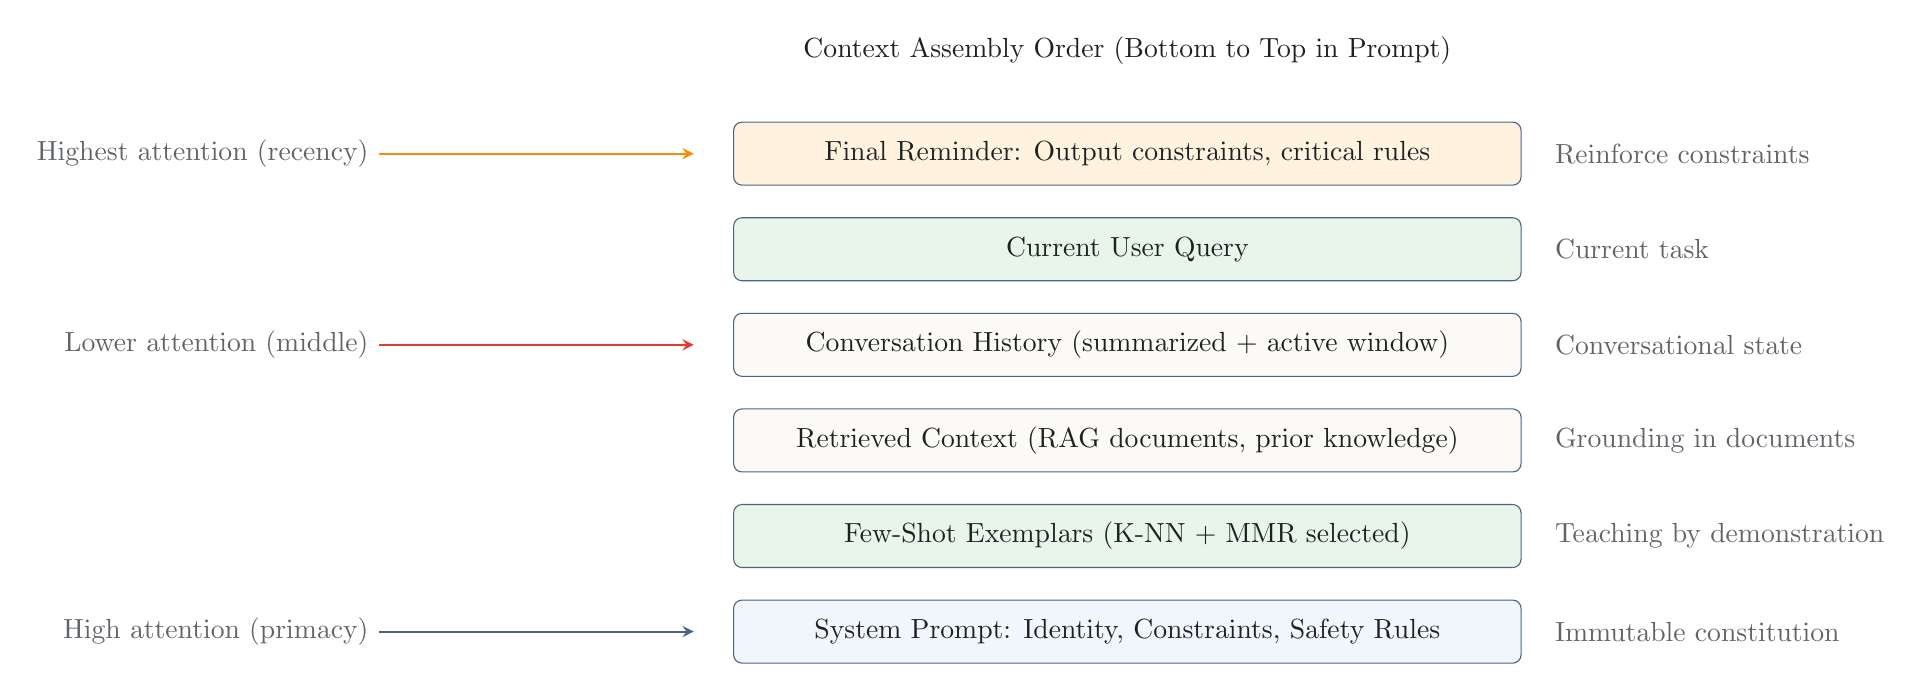
\begin{tikzpicture}[
  node distance=0.4cm,
  layer/.style={
    rectangle,
    draw=border-definition,
    fill=bg-definition,
    rounded corners=3pt,
    minimum width=10cm,
    minimum height=0.8cm,
    font=\small,
    text=text-primary
  },
  arrow/.style={
    ->,
    >=stealth,
    thick,
    draw=text-secondary
  },
  label/.style={
    font=\footnotesize\itshape,
    text=text-muted
  }
]

% Layers from bottom to top
\node[layer, fill=definition-light] (system) {System Prompt: Identity, Constraints, Safety Rules};
\node[layer, fill=example-light, above=of system] (examples) {Few-Shot Exemplars (K-NN + MMR selected)};
\node[layer, fill=note-light, above=of examples] (retrieved) {Retrieved Context (RAG documents, prior knowledge)};
\node[layer, fill=note-light, above=of retrieved] (history) {Conversation History (summarized + active window)};
\node[layer, fill=example-light, above=of history] (query) {Current User Query};
\node[layer, fill=key-light, above=of query] (reminder) {Final Reminder: Output constraints, critical rules};

% Arrows indicating attention
\draw[arrow, draw=definition-base] ([xshift=-4.5cm]system.west) -- ([xshift=-0.5cm]system.west)
  node[label, pos=0, left] {High attention (primacy)};
\draw[arrow, draw=caution-base] ([xshift=-4.5cm]history.west) -- ([xshift=-0.5cm]history.west)
  node[label, pos=0, left] {Lower attention (middle)};
\draw[arrow, draw=key-base] ([xshift=-4.5cm]reminder.west) -- ([xshift=-0.5cm]reminder.west)
  node[label, pos=0, left] {Highest attention (recency)};

% Right-side labels
\node[label, right=0.3cm of system] {Immutable constitution};
\node[label, right=0.3cm of examples] {Teaching by demonstration};
\node[label, right=0.3cm of retrieved] {Grounding in documents};
\node[label, right=0.3cm of history] {Conversational state};
\node[label, right=0.3cm of query] {Current task};
\node[label, right=0.3cm of reminder] {Reinforce constraints};

% Title
\node[above=0.6cm of reminder, font=\bfseries\small, text=text-primary] {Context Assembly Order (Bottom to Top in Prompt)};

\end{tikzpicture}
}
  \caption{Context assembly order for multi-turn conversations. Place the system prompt and critical constraints at the beginning (primacy zone), context and history in the middle, and the current query with reminders at the end (recency zone) for maximum retention.}
  \label{fig:llmB-context-assembly}
\end{figure}

\paragraph{Example: Financial Compliance.} Consider a financial advisory system where legal disclaimers are mandatory:

\begin{quote}
\texttt{[System: You are a financial information assistant...]}

\texttt{[History of conversation...]}

\texttt{[User: What stocks should I buy?]}

\texttt{[Reminder: You must not provide personalized investment advice. If asked, explain that you provide educational information only and recommend consulting a licensed financial advisor. Always include a disclaimer.]}
\end{quote}

The final reminder, placed immediately before generation, increases compliance probability.

\subsection{Safety, Guardrails, and Constitutional AI}
\label{sec:llmB-safety}

As conversational agents become more capable and autonomous, the risk of harmful behaviors increases. Systems may generate toxic content, facilitate harmful activities, or reveal sensitive information. Governance controls must be baked into the conversational loop, distinct from the model's raw capabilities.

\subsubsection{Guardrails: Classification-Based Defense}

\keyterm{Guardrails} are typically implemented as separate, lightweight classification models that scan both inputs and outputs \parencite{dong2024guardrails, inan2023llamaguard}. These guardrail models effectively ``wrap'' the main LLM:

\begin{enumerate}
  \item \textbf{Input check}: Before the user input reaches the LLM, the guardrail checks for malicious intent, prohibited requests, or policy violations
  \item \textbf{Generation}: If input passes, the main LLM generates a response
  \item \textbf{Output check}: Before returning to the user, the guardrail checks the response for policy violations
  \item \textbf{Intervention}: If a violation is detected at either stage, the guardrail intercepts the message and replaces it with a standard refusal or safe response
\end{enumerate}

\begin{highlightbox}[title={Defense in Depth}]
Robust systems implement multiple layers of protection:
\begin{itemize}
  \item \textbf{System prompt}: First line of defense, establishing behavioral boundaries
  \item \textbf{Input guardrails}: Catch malicious inputs before they reach the model
  \item \textbf{Output guardrails}: Catch harmful generations before they reach the user
  \item \textbf{Audit logging}: Record all interactions for review and incident response
  \item \textbf{Human escalation}: Mechanism to route sensitive queries to human reviewers
\end{itemize}
\end{highlightbox}

\begin{highlightbox}[title={From Guardrails to Governance}]
Guardrails evolve into governance surfaces in agentic systems. Our companion volume, \textit{Agentic AI in Law and Finance}, addresses how to design agents that can be audited, overridden, and controlled---extending these safety concepts to autonomous operation.
\end{highlightbox}

\subsubsection{Constitutional AI}

A more advanced and theoretically robust approach is \keyterm{Constitutional AI} (CAI), pioneered by Anthropic \parencite{bai2022constitutional}. Instead of relying solely on Reinforcement Learning from Human Feedback (RLHF)---which is hard to scale, expensive, and can encode implicit human biases---CAI uses a ``constitution'' of explicit principles (e.g., ``Please choose the response that is most helpful, honest, and harmless'').

The CAI process involves a self-supervised mechanism:

\begin{enumerate}
  \item \textbf{Generation}: The model generates responses to prompts, including potentially harmful ones
  \item \textbf{Critique}: The model critiques its own response based on the constitution (e.g., ``Did this response encourage violence?'')
  \item \textbf{Revision}: The model revises the response to be compliant
  \item \textbf{Training}: The model is fine-tuned on these revised, safe traces
\end{enumerate}

This method creates a conversational agent that is ``aligned'' via explicit rules rather than implicit human preferences, making the model's refusal behavior more explainable, consistent, and robust against adversarial attacks.

\subsubsection{Practical Safety Prompts}

For practitioners without access to fine-tuning, safety must be implemented through prompt design:

\begin{itemize}
  \item \textbf{Explicit prohibitions}: ``Do not provide medical diagnoses, legal advice, or recommendations to harm.''
  \item \textbf{Uncertainty acknowledgment}: ``When uncertain, acknowledge limitations and recommend consulting an expert.''
  \item \textbf{Refusal patterns}: ``If asked to do X, respond with Y.''
  \item \textbf{Clarification triggers}: ``If the request is ambiguous or potentially harmful, ask for clarification rather than assuming intent.''
\end{itemize}

\paragraph{Safety and Reasoning.} Note that revealing the model's reasoning (if you use techniques like chain-of-thought, discussed in \Cref{sec:llmB-reason}) can sometimes conflict with safety. Often we keep detailed reasoning hidden precisely so the model can deliberate freely---even consider and reject a potentially harmful action---without ever exposing a harmful thought to the user. For example, an LLM might internally reason ``The user is asking how to do something dangerous---I should refuse,'' but you wouldn't want it to reply with that reasoning visible. You just want it to refuse. Thus, part of safety is deciding which parts of the model's process to keep private.

\subsection{Implementation Patterns for Professional Applications}

Before synthesizing the complete architecture, it is worth examining specific implementation patterns that arise in legal and financial contexts. These domains present unique challenges that generic chatbot architectures do not address.

\subsubsection{Legal Conversation Patterns}

Legal applications require careful attention to several domain-specific constraints:

\paragraph{Privilege Protection.} Attorney-client privilege considerations must be embedded in the system architecture. The conversational system must never expose privileged information to unauthorized parties, even in error messages or debugging logs. This requires:

\begin{itemize}
  \item Separate storage for privileged and non-privileged conversation content
  \item Access controls that verify privilege status before retrieving historical context
  \item Audit trails that distinguish between privileged and non-privileged interactions
  \item Memory strategies that respect privilege boundaries when summarizing conversations
\end{itemize}

\paragraph{Jurisdictional Awareness.} Legal analysis varies significantly by jurisdiction. A conversational legal assistant must maintain awareness of:

\begin{itemize}
  \item The governing jurisdiction for the matter under discussion
  \item When the user shifts jurisdictional context (e.g., ``What about under California law?'')
  \item When an answer depends on jurisdictional variation and should note alternatives
  \item Conflict of laws considerations when multiple jurisdictions are relevant
\end{itemize}

These requirements influence memory architecture. The system should pin the primary jurisdiction in persistent memory, flag jurisdictional shifts as significant context changes, and retrieve jurisdiction-specific precedents when constructing prompts.

\paragraph{Temporal Sensitivity.} Legal rules change. A conversation about employment law may produce different answers depending on whether it occurred before or after a significant regulatory change. Conversational legal systems must:

\begin{itemize}
  \item Track the effective dates of legal rules referenced in responses
  \item Warn users when advice may be affected by recent or pending legal changes
  \item Maintain metadata about when information was last verified
  \item Consider whether to use retrieval to verify current legal status
\end{itemize}

\subsubsection{Financial Conversation Patterns}

Financial applications present their own distinct requirements:

\paragraph{Regulatory Boundaries.} Financial services are heavily regulated, and conversational AI must navigate complex compliance requirements:

\begin{itemize}
  \item Distinguishing between general information and personalized advice (which may trigger registration requirements)
  \item Ensuring disclosures are presented when required
  \item Maintaining records as required by securities, banking, or insurance regulations
  \item Avoiding forward-looking statements that could constitute market manipulation
\end{itemize}

\paragraph{Numerical Precision.} Financial conversations frequently involve numerical data where precision matters:

\begin{itemize}
  \item Currency amounts should be tracked with appropriate precision
  \item Percentages, ratios, and rates must be consistently formatted
  \item The system should clarify ambiguous numerical references (``Did you mean 3\% annually or monthly?'')
  \item Calculations should be verified, ideally through tool use rather than model inference
\end{itemize}

\paragraph{Client Risk Profiling.} Financial conversations often need to consider the client's risk profile, which should be:

\begin{itemize}
  \item Established early in the conversation or retrieved from persistent storage
  \item Updated when the client indicates changed circumstances
  \item Consulted before providing any investment-related information
  \item Protected as sensitive personal information
\end{itemize}

\subsubsection{Multi-Session Continuity}

Many professional applications span multiple conversation sessions. A client may return days or weeks later expecting the assistant to remember prior discussions. This requires:

\paragraph{Session Bridging.} When a user returns, the system must efficiently reconstruct relevant context:

\begin{itemize}
  \item Retrieve high-level summaries of prior sessions
  \item Identify topics that may be relevant to the new session (based on initial user message)
  \item Load pinned facts and persistent preferences
  \item Present a natural transition (``Welcome back. When we last spoke, we were discussing...'')
\end{itemize}

\paragraph{Context Staleness.} Prior conversation context may become stale:

\begin{itemize}
  \item Facts discussed months ago may no longer be accurate
  \item The user's situation may have changed
  \item Regulatory requirements may have evolved
  \item Market conditions discussed previously may be outdated
\end{itemize}

Systems should track context freshness and prompt users to confirm critical facts when resuming long-dormant conversations.

\paragraph{Archival and Retrieval.} Professional contexts often require conversation archival:

\begin{itemize}
  \item Legal hold requirements may prevent deletion of relevant conversations
  \item Compliance auditors may need to search historical conversations
  \item Users may need to reference prior discussions for their own records
  \item The system itself may need to retrieve historical context for current queries
\end{itemize}

These requirements influence storage architecture, retention policies, and search capabilities.

\subsection{Putting It Together: A Conversational Architecture}

To synthesize this section, consider the complete architecture of a production conversational system:

\begin{definitionbox}[title={Conversational System Components}]
\begin{enumerate}
  \item \textbf{Orchestration Layer}: Manages state, constructs prompts, handles tool calls
  \item \textbf{Memory Store}: Persists conversation history, embeddings, pinned facts
  \item \textbf{Retrieval System}: Searches memory and external knowledge for relevant context
  \item \textbf{Input Guardrails}: Classifies user input for policy compliance
  \item \textbf{LLM}: Generates responses given the constructed prompt
  \item \textbf{Output Guardrails}: Classifies model output for policy compliance
  \item \textbf{Audit System}: Logs all interactions for compliance and debugging
\end{enumerate}
\end{definitionbox}

Each component plays a role in maintaining the illusion of a coherent, stateful, and safe conversational agent built on a fundamentally stateless foundation. The choices you make at each layer---what to remember, where to place instructions, how to structure guardrails---determine the reliability and safety of your system.

With the mechanics of conversational state established, we now turn to the second major challenge: how to elicit structured reasoning from these systems.

\input{sections/03-reasoning-patterns}
% =============================================================================
% Strategy Selection — Conversations & Reasoning
% Purpose: Decision framework for selecting strategies based on constraints
% Label: sec:llmB-strategy
% =============================================================================

\section{Choosing Strategies Under Constraints}
\label{sec:llmB-strategy}

The selection of a conversational model design and reasoning pattern is not a binary choice but a multi-dimensional optimization problem. Every application operates under constraints---time, cost, risk tolerance, accuracy requirements---and the optimal strategy depends on how you weight these factors. In this section, we synthesize the patterns discussed earlier into a practical decision framework.

\subsection{The Decision Matrix}

Different tasks call for different approaches. The following matrix provides guidance based on task type and requirements:

\begin{center}
\begin{tabular}{>{\raggedright}p{3cm}p{3.5cm}p{3cm}p{4.5cm}}
\toprule
\textbf{Task Type} & \textbf{Recommended Strategy} & \textbf{Context/Memory} & \textbf{Rationale} \\
\midrule
Chatbots / Creative Writing & Zero-shot or few-shot & Sliding window / Summarization & Latency is critical. Reasoning errors are low-risk. \\
\addlinespace
Math Tutoring / Coding & Chain-of-Thought & K-NN few-shot selection & Precision is key. Users tolerate slight delay for correctness. \\
\addlinespace
Medical / Financial Analysis & Self-Consistency & Vector retrieval (high recall) & \textbf{High risk}. Error cost outweighs compute cost. \\
\addlinespace
Research Assistants & ReAct & Long-term vector memory & Model must interact with tools for real-time data. \\
\addlinespace
Complex Planning / Discovery & Tree of Thoughts & Full context replay & Exploration is needed. High latency acceptable. \\
\bottomrule
\end{tabular}
\end{center}

\subsection{The Four Dimensions of Strategy Selection}

When selecting a strategy, consider four key dimensions:

\subsubsection{Accuracy Requirements}

\begin{itemize}
  \item \textbf{Low-stakes}: Casual conversation, creative writing, brainstorming. Hallucinations are tolerable; speed matters more.
  \item \textbf{Medium-stakes}: Educational content, summarization, drafting. Errors are undesirable but not catastrophic; can be caught in review.
  \item \textbf{High-stakes}: Legal advice, medical diagnosis, financial recommendations. Errors can cause real harm; maximum reliability required.
\end{itemize}

\begin{keybox}[title={High-Stakes Decision Rule}]
For high-stakes applications:
\begin{enumerate}
  \item Always use structured reasoning (CoT or better)
  \item Consider self-consistency for critical determinations
  \item Ground in external sources (ReAct + retrieval)
  \item Include human review in the workflow
  \item Log everything for audit
\end{enumerate}
\end{keybox}

\subsubsection{Latency Tolerance}

\begin{itemize}
  \item \textbf{Real-time} ($<$ 2 seconds): Chatbots, autocomplete, live assistance. Use direct prompting; minimize reasoning overhead.
  \item \textbf{Interactive} (2--30 seconds): Research queries, analysis, document review. CoT and single-pass retrieval acceptable.
  \item \textbf{Batch/Offline} ($>$ 30 seconds): Deep analysis, report generation, complex planning. Full self-consistency, ToT/GoT viable.
\end{itemize}

\subsubsection{Cost Sensitivity}

\begin{itemize}
  \item \textbf{Cost-sensitive}: High-volume consumer applications. Minimize tokens; use smaller models where possible.
  \item \textbf{Moderate budget}: Professional tools with per-query value. Invest in accuracy for high-value queries.
  \item \textbf{Budget unconstrained}: Mission-critical applications. Maximize accuracy regardless of cost.
\end{itemize}

The cost of self-consistency scales linearly with samples ($k$ samples = $k \times$ base cost). Token-efficient techniques like Chain of Draft can reduce CoT overhead by 40\%.

\subsubsection{Explainability Requirements}

\begin{itemize}
  \item \textbf{Black-box acceptable}: Internal tools, automation. Hide reasoning for simplicity.
  \item \textbf{Explainability preferred}: Professional tools. Offer reasoning on request.
  \item \textbf{Explainability mandatory}: Regulated domains (finance, healthcare, legal). Must show reasoning for compliance.
\end{itemize}

\subsection{Context Assembly: The Final Step}

Many conversational failures are, at their root, \emph{context failures}. Before the model even begins to reason, you must construct the prompt correctly. Here is a systematic approach:

\subsubsection{The Context Assembly Recipe}

Assemble your prompt in this order:

\begin{enumerate}
  \item \textbf{System Prompt}: Identity, constraints, safety rules
  \item \textbf{Few-Shot Exemplars}: Selected via similarity (K-NN) and diversity (MMR)
  \item \textbf{Retrieved Context}: Documents, data, or prior knowledge (RAG)
  \item \textbf{Conversation History}: Summarized older turns + recent active window
  \item \textbf{Current User Query}: The actual question or request
  \item \textbf{Final Reminder}: Output constraints, format requirements, critical rules
\end{enumerate}

\begin{highlightbox}[title={Why Order Matters}]
Due to the ``Lost in the Middle'' phenomenon:
\begin{itemize}
  \item Information at the \textbf{start} (system prompt) is retained well
  \item Information in the \textbf{middle} (retrieved context, history) is partially degraded
  \item Information at the \textbf{end} (query + reminder) receives highest attention
\end{itemize}
Place your most critical constraints at both the start AND end.
\end{highlightbox}

\subsubsection{Token Budgeting in Practice}

Before each call, verify your token allocation:

\begin{enumerate}
  \item \textbf{Check total capacity}: Know your model's context limit (8K, 32K, 128K, etc.)
  \item \textbf{Reserve for output}: Allocate 1K--4K tokens for the response, depending on expected length
  \item \textbf{Allocate components}: Divide remaining budget across system prompt, examples, context, and history
  \item \textbf{Truncate if necessary}: If over budget, compress history first (summarize), then reduce retrieved context (re-rank for relevance), then reduce examples
  \item \textbf{Never truncate}: System prompt or final reminder (these are non-negotiable)
\end{enumerate}

\subsection{Application-Specific Guidance}

\subsubsection{Legal Applications}

\begin{keybox}[title={Legal AI Strategy Recommendations}]
\begin{itemize}
  \item \textbf{Legal research}: ReAct with access to case databases; cite all sources
  \item \textbf{Document review}: Few-shot with domain-specific examples; CoT for analysis
  \item \textbf{Contract analysis}: CoT with explicit checklist prompting; self-consistency for critical clauses
  \item \textbf{Compliance questions}: ReAct for regulatory lookups; never rely solely on training data for current regulations
  \item \textbf{Always}: Include disclaimers; acknowledge limitations; recommend human review
\end{itemize}
\end{keybox}

\subsubsection{Financial Applications}

\begin{keybox}[title={Financial AI Strategy Recommendations}]
\begin{itemize}
  \item \textbf{Market data queries}: ReAct with API access; never use training data for prices
  \item \textbf{Risk analysis}: Self-consistency for quantitative assessments
  \item \textbf{Portfolio suggestions}: CoT with explicit constraint checking (risk tolerance, time horizon)
  \item \textbf{Regulatory queries}: ReAct for up-to-date rule lookups (SEC, FINRA, etc.)
  \item \textbf{Always}: Include suitability disclaimers; distinguish information from advice
\end{itemize}
\end{keybox}

\subsubsection{Customer-Facing Applications}

For general-purpose assistants where latency and user experience matter:

\begin{itemize}
  \item Use direct prompting or simple few-shot for routine queries
  \item Escalate to CoT only for detected complexity (e.g., multi-part questions)
  \item Implement guardrails at both input and output stages
  \item Keep responses concise; offer to elaborate if user requests
  \item Use sliding window + summary for conversation history
\end{itemize}

\subsection{Governance Implications}

Your choice of reasoning strategy has governance implications:

\paragraph{Auditability.} Strategies that produce reasoning traces (CoT, ReAct) provide audit trails. Even if you hide traces from users, log them for compliance review.

\paragraph{Explainability.} Regulated industries may require explanations. CoT provides this naturally; private scratchpads can be disclosed on request.

\paragraph{Reproducibility.} Self-consistency with majority voting is more reproducible than single-sample generation (which varies with temperature). For regulated applications, consider deterministic settings (temperature = 0) or explicit seed values.

\paragraph{Version Control.} Track your system prompts, few-shot examples, and strategy configurations. When issues arise, you need to reproduce the exact conditions that produced a problematic output.

\begin{highlightbox}[title={What Part III Covers}]
This chapter provides foundational strategies. Part III (Governing AI Agents) expands on:
\begin{itemize}
  \item Comprehensive governance frameworks for AI deployment
  \item Regulatory requirements across jurisdictions
  \item Risk assessment methodologies
  \item Incident response and escalation protocols
  \item Organizational structures for AI oversight
\end{itemize}
\end{highlightbox}

\subsection{Decision Flowchart}

When facing a new task, use this simplified decision process:

\begin{enumerate}
  \item \textbf{Assess stakes}: Is this high-risk (legal, medical, financial) or low-risk?
  \item \textbf{Check data needs}: Does the task require current information beyond training data?
  \item \textbf{Evaluate complexity}: Is multi-step reasoning required?
  \item \textbf{Consider constraints}: What are the latency and cost limits?
  \item \textbf{Select pattern}:
  \begin{itemize}
    \item Low-risk, simple, real-time → Direct prompting
    \item Low-risk, complex, real-time → CoT
    \item Any risk, needs current data → ReAct
    \item High-risk, complex → Self-consistency + CoT
    \item High-value, complex, offline → ToT/GoT
  \end{itemize}
  \item \textbf{Design memory}: Choose appropriate context management for conversation length
  \item \textbf{Implement guardrails}: Add safety layers appropriate to risk level
  \item \textbf{Test and iterate}: Validate on representative examples before deployment
\end{enumerate}

The right strategy is the \emph{simplest one that meets your accuracy and safety requirements}. Over-engineering wastes resources and can introduce unnecessary complexity. Start simple, measure results, and add sophistication only where needed.

\subsection{Case Studies in Strategy Selection}

To illustrate how these principles apply in practice, consider the following scenarios drawn from legal and financial contexts.

\subsubsection{Case Study 1: Legal Research Assistant}

\textbf{Scenario}: A law firm wants to deploy an AI assistant that helps associates research case law and statutes relevant to client matters.

\textbf{Analysis}:
\begin{itemize}
  \item \textbf{Stakes}: High. Incorrect legal citations could embarrass the firm or, worse, lead to malpractice.
  \item \textbf{Data needs}: Critical. Legal research requires access to current case law and statutes.
  \item \textbf{Complexity}: High. Legal analysis requires multi-step reasoning, analogy, and application of rules to facts.
  \item \textbf{Constraints}: Moderate latency tolerance (research tasks are not real-time); cost is acceptable for high-value work.
\end{itemize}

\textbf{Recommended Strategy}:
\begin{itemize}
  \item \textbf{ReAct with retrieval}: Absolutely essential. The model must search legal databases rather than rely on training data.
  \item \textbf{Chain-of-thought with IRAC structure}: Produce reasoning traces that follow the Issue-Rule-Application-Conclusion format familiar to legal professionals.
  \item \textbf{Self-consistency}: For important conclusions, run multiple reasoning paths and verify agreement.
  \item \textbf{Private scratchpad}: Keep exploratory reasoning hidden; show only polished analysis to users.
  \item \textbf{Citation verification guardrail}: Before presenting any case citation, verify it exists and check its subsequent history.
\end{itemize}

\textbf{Memory Configuration}: Long conversations tracking matter details. Pin client facts, governing jurisdiction, and key deadlines. Use recursive summarization for extended research sessions.

\subsubsection{Case Study 2: Financial News Summarization}

\textbf{Scenario}: An investment firm wants to automatically summarize daily financial news for portfolio managers.

\textbf{Analysis}:
\begin{itemize}
  \item \textbf{Stakes}: Moderate. Summaries inform but don't directly drive trades; errors are caught in review.
  \item \textbf{Data needs}: Critical. News summarization inherently requires current content.
  \item \textbf{Complexity}: Moderate. Summarization is well within LLM capabilities.
  \item \textbf{Constraints}: Daily batch processing; cost-sensitive due to high volume; moderate latency tolerance.
\end{itemize}

\textbf{Recommended Strategy}:
\begin{itemize}
  \item \textbf{ReAct with news retrieval}: Fetch articles from trusted sources.
  \item \textbf{Simple chain-of-thought}: Identify key points, note market implications, synthesize.
  \item \textbf{Single-pass generation}: Self-consistency is overkill for summarization.
  \item \textbf{Visible reasoning}: Summary structure naturally shows reasoning.
  \item \textbf{Topic-based guardrails}: Flag articles about portfolio companies for human attention.
\end{itemize}

\textbf{Memory Configuration}: Each news item is independent; minimal cross-article context needed. Consider tagging summaries with topics for later retrieval.

\subsubsection{Case Study 3: Client Risk Assessment Chatbot}

\textbf{Scenario}: A wealth management firm wants a chatbot that gathers client information and produces preliminary risk assessments.

\textbf{Analysis}:
\begin{itemize}
  \item \textbf{Stakes}: High. Regulatory requirements around suitability assessments; fiduciary duties.
  \item \textbf{Data needs}: Low. Assessment based on client-provided information, not external data.
  \item \textbf{Complexity}: Moderate. Structured questionnaire with conditional logic.
  \item \textbf{Constraints}: Real-time (conversation with client); must feel natural and responsive.
\end{itemize}

\textbf{Recommended Strategy}:
\begin{itemize}
  \item \textbf{Direct prompting with few-shot examples}: Model appropriate conversational patterns for gathering information.
  \item \textbf{Simple chain-of-thought for classification}: Show reasoning for risk category assignment.
  \item \textbf{No retrieval}: Assessment based on conversation content only.
  \item \textbf{Strict guardrails}: Never provide investment advice; only gather information and classify.
  \item \textbf{Mandatory human review}: Assessment is preliminary; always routed to advisor for confirmation.
\end{itemize}

\textbf{Memory Configuration}: Track all client responses in current session. Pin stated risk tolerance and investment horizon. Clear session-specific context between clients but maintain templates.

\subsubsection{Case Study 4: Contract Review Workflow}

\textbf{Scenario}: A corporate legal department wants AI assistance reviewing vendor contracts for risk terms.

\textbf{Analysis}:
\begin{itemize}
  \item \textbf{Stakes}: High. Missing a problematic clause could expose the company to significant liability.
  \item \textbf{Data needs}: Moderate. Contract review is primarily about the document itself, but comparison to company playbook may require retrieval.
  \item \textbf{Complexity}: High. Contracts require careful parsing, cross-reference of definitions, and risk assessment.
  \item \textbf{Constraints}: Batch processing acceptable; thoroughness valued over speed.
\end{itemize}

\textbf{Recommended Strategy}:
\begin{itemize}
  \item \textbf{Tree of Thoughts}: Explore the contract systematically by section, considering multiple interpretations of ambiguous language.
  \item \textbf{ReAct for playbook comparison}: Retrieve company's standard positions and risk thresholds for each clause type.
  \item \textbf{Self-consistency for risk ratings}: Multiple evaluations of high-risk clauses to verify assessment.
  \item \textbf{Structured output}: Produce standardized risk reports with clause-by-clause analysis.
  \item \textbf{Escalation triggers}: Automatically flag contracts meeting certain criteria for senior review.
\end{itemize}

\textbf{Memory Configuration}: Contract context must persist throughout review. Pin key definitions and parties. Maintain session with all identified issues for final summary.

\subsubsection{Lessons from Case Studies}

These examples illustrate several recurring patterns:

\begin{keybox}[title={Strategy Selection Principles}]
\begin{enumerate}
  \item \textbf{Match stakes to verification}: Higher stakes justify more expensive verification strategies (self-consistency, human review).
  \item \textbf{Use retrieval when data matters}: Any task involving facts beyond training data requires tool-augmented reasoning.
  \item \textbf{Structure reasoning for the audience}: Legal tasks benefit from IRAC; financial tasks from structured scenarios.
  \item \textbf{Consider the full workflow}: AI is rarely the final word in professional contexts; design for handoff.
  \item \textbf{Start simple}: Begin with the simplest strategy that might work; add complexity only when measurement shows it's needed.
\end{enumerate}
\end{keybox}


% =============================================================================
% Synthesis — Conversations & Reasoning
% Purpose: Integration of concepts and bridge to next chapters
% Label: sec:llmB-synthesis
% =============================================================================

\section{Synthesis: From Stateless Models to Cognitive Systems}
\label{sec:llmB-synthesis}

We have moved from viewing the LLM as a simple text predictor to seeing it as the kernel of a \emph{cognitive operating system}---one that requires explicit memory management, structured reasoning topologies, and rigorous safety constitutions to function effectively in professional settings.

\subsection{The Three Pillars of Conversational AI}

This chapter has established three foundational pillars for building reliable conversational systems:

\begin{definitionbox}[title={Pillar 1: State Management}]
\textbf{Creating memory in a memoryless system.}

Since LLMs are fundamentally stateless, maintaining conversational coherence requires an orchestration layer that:
\begin{itemize}
  \item Constructs prompts with appropriate role separation (system, user, assistant)
  \item Manages context windows through sliding windows, summarization, or vector retrieval
  \item Places critical instructions strategically to combat attention degradation
  \item Implements safety guardrails at input and output stages
\end{itemize}
The illusion of memory is created by careful context construction, not by the model itself.
\end{definitionbox}

\begin{definitionbox}[title={Pillar 2: Structured Reasoning}]
\textbf{Moving beyond pattern matching to genuine inference.}

Complex professional tasks require reasoning capabilities that raw LLMs lack. We achieve this through:
\begin{itemize}
  \item \textbf{Chain-of-Thought}: Externalizing intermediate reasoning steps
  \item \textbf{Self-Consistency}: Sampling multiple paths and voting on answers
  \item \textbf{Tool Augmentation}: Grounding in external data sources (ReAct)
  \item \textbf{Exploration}: Tree and Graph of Thoughts for complex planning
  \item \textbf{Self-Reflection}: Critique and revision loops for quality improvement
\end{itemize}
Each technique trades off accuracy, latency, and cost differently.
\end{definitionbox}

\begin{definitionbox}[title={Pillar 3: Strategic Selection}]
\textbf{Matching techniques to requirements.}

No single approach works for all tasks. Effective deployment requires:
\begin{itemize}
  \item Assessing the stakes (risk tolerance for errors)
  \item Evaluating latency and cost constraints
  \item Determining explainability requirements
  \item Selecting the simplest strategy that meets requirements
  \item Implementing appropriate governance controls
\end{itemize}
The goal is not maximum sophistication but appropriate sophistication.
\end{definitionbox}

\subsection{Key Takeaways}

\begin{keybox}[title={Chapter Summary}]
\begin{enumerate}
  \item \textbf{Conversations require state management}: The model doesn't remember anything; your application must manage context explicitly through prompt construction.

  \item \textbf{Position matters}: Due to the ``Lost in the Middle'' phenomenon, place critical information at the start and end of prompts, not buried in the middle.

  \item \textbf{Reasoning improves accuracy}: Chain-of-thought and related techniques dramatically improve performance on complex tasks, but at the cost of additional tokens and latency.

  \item \textbf{Tools ground in reality}: ReAct-style approaches reduce hallucinations by connecting the model to real-time data sources, essential for legal and financial applications.

  \item \textbf{Multiple paths increase reliability}: Self-consistency (sampling multiple reasoning chains and voting) provides robust answers for high-stakes decisions.

  \item \textbf{Safety is layered}: Effective guardrails combine system prompts, input/output classifiers, and human escalation paths.

  \item \textbf{Simpler is often better}: Use the minimum necessary complexity; over-engineering wastes resources and can introduce new failure modes.
\end{enumerate}
\end{keybox}

\subsection{The Integration of State and Reasoning}

These pillars are not independent. Effective reasoning often requires sophisticated state management:

\begin{itemize}
  \item \textbf{ReAct} requires maintaining state across thought-action-observation cycles
  \item \textbf{Self-consistency} requires aggregating results across multiple independent runs
  \item \textbf{Tree/Graph of Thoughts} requires tracking branching states and backtracking
  \item \textbf{Self-reflection} requires maintaining drafts and critiques across iterations
\end{itemize}

Similarly, state management decisions affect reasoning capabilities:

\begin{itemize}
  \item \textbf{Context window limits} constrain how much reasoning trace can be maintained
  \item \textbf{Memory strategies} determine what prior reasoning is available for reference
  \item \textbf{Few-shot example selection} primes the reasoning patterns the model will employ
\end{itemize}

Understanding this interplay is essential for designing robust conversational systems.

\subsection{What We Have Not Covered}

This chapter focused on the fundamental mechanics of conversations and reasoning. Several important topics are deferred to subsequent chapters:

\begin{highlightbox}[title={Covered in Later Chapters}]
\begin{itemize}
  \item \textbf{Structured Outputs} (Chapter~4): Forcing models to produce JSON, XML, or other schema-conformant outputs
  \item \textbf{Tool Use and Function Calling} (Chapter~5): Implementation details for integrating external APIs and tools
  \item \textbf{Multimodal Inputs} (Chapter~6): Processing PDFs, tables, audio, and visual content
  \item \textbf{Evaluation and Optimization} (Chapter~7): Systematic improvement of prompts and pipelines
  \item \textbf{Agent Architectures and Governance}: Covered in our companion volume, \textit{Agentic AI in Law and Finance}
\end{itemize}
\end{highlightbox}

\begin{keybox}[title={Continuing Your Journey: From Conversations to Agents}]
This chapter established the foundations for conversational AI and structured reasoning. These techniques become building blocks for agentic systems.

Our companion volume, \textit{Agentic AI in Law and Finance}, provides a rigorous conceptual framework for distinguishing genuine agents from sophisticated tools, and translates these concepts into architectural questions that guide agent design---from triggers to governance.

The memory strategies, reasoning patterns, and safety mechanisms introduced here scale to autonomous systems that iterate, adapt, and take action in the world.
\end{keybox}

\subsection{Bridge to Structured Outputs and Tools}

The techniques in this chapter prepare you for the next level of LLM capability: producing structured, machine-readable outputs and interacting with external systems.

\paragraph{From Free Text to Schemas.} Reasoning produces answers, but professional applications often require those answers in specific formats. Chapter~4 covers techniques for constraining model outputs to conform to JSON schemas, legal citation formats, financial report structures, and other domain-specific templates.

\paragraph{From Conversations to Actions.} We introduced ReAct as a reasoning pattern, but we only sketched how tool calls actually work. Chapter~5 explains the mechanics of function calling, API integration, and the protocols that enable models to take actions in the world.

\paragraph{From Text to Documents.} Professional work involves real documents: PDFs with complex layouts, financial statements with tables, contracts with exhibits. Chapter~6 extends these techniques to multimodal inputs.

With the foundations of state management and reasoning established, you are ready to explore how LLMs can produce structured outputs, use tools, and integrate with the broader ecosystem of professional applications.


% =============================================================================
% Further Learning — Providing Context
% Purpose: Annotated bibliography for context and retrieval topics
% Label: sec:llmB2-further
% =============================================================================

\section{Further Learning}
\label{sec:llmB2-further}

This section provides an annotated guide to resources for readers who wish to deepen their understanding of context provision techniques, in-context learning, and retrieval-augmented generation.

\subsection{In-Context Learning Foundations}
\label{sec:llmB2-further-icl}

\paragraph{The GPT-3 Paper.}
\fullcite{brown2020fewshot}

The GPT-3 paper introduced few-shot learning as a practical paradigm, demonstrating that large models can learn from examples in the prompt without weight updates. Essential for understanding why in-context learning works and its scaling properties.

\paragraph{Rethinking the Role of Demonstrations.}
\fullcite{min2022rethinking}

This paper challenges assumptions about few-shot learning, showing that models often rely more on the format of demonstrations than their content. Important for understanding that in-context learning is not classical learning but rather a form of task specification.

\paragraph{What Can Transformers Learn In-Context?}
\fullcite{garg2022transformers}

A theoretical analysis of in-context learning as implicit meta-learning. Helps explain the mechanisms by which Transformers adapt to examples in the prompt.

\subsection{Retrieval-Augmented Generation}
\label{sec:llmB2-further-rag}

\paragraph{The Original RAG Paper.}
\fullcite{lewis2020rag}

The foundational paper introducing retrieval-augmented generation. Establishes the pattern of combining parametric knowledge (model weights) with non-parametric knowledge (retrieved documents). Essential reading for understanding the RAG architecture.

\paragraph{Dense Passage Retrieval.}
\fullcite{karpukhin2020dpr}

Introduces learned dense embeddings for passage retrieval, demonstrating that semantic embeddings outperform keyword methods for many tasks. Foundation for understanding modern embedding-based retrieval.

\paragraph{Lost in the Middle.}
\fullcite{liu2023lostmiddle}

Documents the U-shaped attention pattern where models struggle to use information positioned in the middle of long contexts. Critical for understanding context window limitations and designing effective retrieval strategies.

\paragraph{ColBERT and Efficient Retrieval.}
\fullcite{khattab2020colbert}

Introduces late interaction for efficient cross-encoder-quality retrieval. Important for understanding production retrieval systems that balance accuracy and latency.

\subsection{Hybrid Search and Retrieval Quality}
\label{sec:llmB2-further-hybrid}

\paragraph{BM25: The Baseline.}
The BM25 algorithm, while dating to the 1990s, remains a strong baseline for keyword retrieval. Understanding BM25 helps explain why hybrid approaches combining keyword and semantic search often outperform either alone. Standard implementations are available in Elasticsearch, Lucene, and dedicated libraries.

\paragraph{Re-ranking for Precision.}
Cross-encoder re-ranking using models like Cohere Rerank or similar architectures can dramatically improve retrieval precision at modest latency cost. The pattern of fast first-stage retrieval followed by expensive re-ranking is standard in production systems.

\subsection{Embeddings and Vector Databases}
\label{sec:llmB2-further-embeddings}

\paragraph{Sentence Transformers.}
\fullcite{reimers2019sentencebert}

Introduces efficient sentence embeddings that enable semantic search. The foundation of most modern embedding approaches for retrieval.

\paragraph{Text and Code Embeddings.}
\fullcite{openai2022embedding}

OpenAI's embedding models (text-embedding-ada-002 and successors) have become standard choices for retrieval. Understanding their properties---including dimensionality, domain coverage, and multilingual support---helps in system design.

\paragraph{Vector Database Selection.}
Production RAG systems require vector databases for efficient similarity search. Options include Pinecone, Weaviate, Qdrant, Milvus, and pgvector (PostgreSQL extension). Selection criteria include scale requirements, hosting preferences, and integration capabilities.

\subsection{Domain-Specific Retrieval}
\label{sec:llmB2-further-domain}

\paragraph{Legal Information Retrieval.}
Legal retrieval has a long history predating LLMs. Traditional systems like Westlaw and LexisNexis incorporate citation analysis, authority ranking, and jurisdictional filtering. Modern legal AI must integrate with or replicate these capabilities.

\paragraph{Financial Document Processing.}
Financial documents present particular challenges: structured tables, standardized formats (XBRL, EDGAR), and regulatory requirements for accuracy. SEC filings, earnings transcripts, and financial statements each require specialized preprocessing.

\subsection{Practical Implementation Guides}
\label{sec:llmB2-further-practical}

\begin{itemize}
  \item \textbf{LangChain Documentation:} Comprehensive framework for building RAG pipelines with retrieval, chunking, and generation components. \url{https://python.langchain.com/docs}

  \item \textbf{LlamaIndex:} Framework focused on data indexing and retrieval for LLM applications. \url{https://docs.llamaindex.ai}

  \item \textbf{Anthropic Cookbook:} Practical guides for Claude including context window management and RAG patterns. \url{https://docs.anthropic.com/cookbook}

  \item \textbf{OpenAI Cookbook:} Implementation examples including retrieval and embedding use cases. \url{https://cookbook.openai.com}
\end{itemize}

\subsection{Staying Current}
\label{sec:llmB2-further-current}

RAG and retrieval techniques evolve rapidly. Resources for staying current:

\begin{itemize}
  \item \textbf{arXiv cs.IR and cs.CL:} New retrieval and NLP research appears as preprints
  \item \textbf{Vendor blogs:} OpenAI, Anthropic, Cohere, and vector database vendors publish implementation guidance
  \item \textbf{Community resources:} The RAG community shares techniques through blog posts, podcasts, and open-source implementations
\end{itemize}

The field moves quickly; techniques from early 2024 may already be superseded. Check publication dates and look for subsequent citations when evaluating sources.


% =============================================================================
% Conclusion — Structured Outputs
% Purpose: Closing summary and handoff to tool use chapter
% Label: sec:llmC2-conclusion
% =============================================================================

\section*{Conclusion}
\addcontentsline{toc}{section}{Conclusion}
\label{sec:llmC2-conclusion}

This chapter addressed a fundamental challenge: transforming probabilistic text generation into deterministic, validated, auditable data. We moved from treating LLMs as conversational tools to deploying them as embedded components within strict data pipelines that professional practice demands.

\subsection*{Key Takeaways}

\paragraph{Structured Outputs Enable Integration.} Free-form text cannot be directly consumed by databases, compliance systems, or analytics pipelines. Structured outputs---schema-constrained JSON, XML, or CSV---transform AI from a conversational curiosity into a production-grade data source. The techniques we examined, from prompt-based formatting to constrained decoding, provide the interface between probabilistic generation and deterministic systems.

\paragraph{Evidence Records Enable Audit.} In professional practice, every claim must be traceable. The Canonical Evidence Record schema captures source, location, quote, jurisdiction, date, and cryptographic hash for every assertion. This transforms opaque AI outputs into auditable artifacts suitable for legal proceedings and regulatory scrutiny.

\paragraph{Production Retrieval Differs from Prototype.} The RAG fundamentals from Chapter~2 are necessary but not sufficient. Production systems require multi-stage retrieval, query rewriting, re-ranking, and continuous quality measurement. A prototype that works 80\% of the time is interesting; a production system that fails 20\% of the time is unacceptable.

\paragraph{Validation is Architectural.} Never trust LLM outputs without validation. Schema validation catches structural errors; semantic validation catches type errors; business rule validation catches domain violations. Implement retry logic, fallback handling, and human escalation paths.

\subsection*{The Core Insight}

The central theme of this chapter is that \textbf{structure enables, not constrains}. Imposing schemas, validation, and evidence requirements does not limit what AI systems can do---it enables them to participate in professional workflows where reliability and auditability are non-negotiable.

An unstructured system produces text that must be read, interpreted, and manually entered. A structured system produces data that flows directly into downstream processes. The difference is not cosmetic; it is architectural.

\subsection*{Looking Forward}

\paragraph{Chapter 5: Tool Use.} With structured outputs established, we extend the model's capabilities to take actions in the world. Function calling enables LLMs to invoke calculators, query databases, search the web, and integrate with enterprise APIs. The structured output foundations from this chapter---schemas, validation, evidence records---apply directly to tool use.

\paragraph{Chapter 6: Multimodal Documents.} We extend structured extraction to the documents professionals actually work with: PDFs with complex layouts, financial statements with tables, charts and visualizations, audio transcripts. The same schema patterns and evidence records apply; we add modality-specific parsing.

\paragraph{Chapter 7: Systematic Improvement.} We treat prompts and pipelines as engineering artifacts subject to evaluation, optimization, and version control. Structured outputs enable quantitative measurement---schema compliance rates, citation accuracy, field extraction precision---that drives systematic improvement.

\subsection*{Final Thoughts}

The journey from experimental chatbot to production system requires discipline. Every output must be validated. Every claim must be traceable. Every component must be versioned. This discipline is not bureaucratic overhead---it is the engineering rigor that makes AI systems suitable for high-stakes professional applications.

You now understand how to constrain LLM outputs to structured formats, how to validate those outputs, and how to maintain evidence records for audit. The next chapter extends these foundations to enable AI systems that act, not just analyze.

\vspace{1em}
\begin{center}
\rule{0.4\textwidth}{0.4pt}
\end{center}



% ============================================================================
% BIBLIOGRAPHY
% ============================================================================

\clearpage
\printbibliography

\end{document}

\usepackage{pgfornament}

% ==========================================================================
% COVER VARIABLES (trim size, bleed, spine width)
% ==========================================================================
% ============================================================================
% COVER VARIABLES - Generated for Lulu wrap cover
% ============================================================================
% Generated: 2025-12-28 19:18:27
% Binding: paperback | Pages: 423
% Paperback Perfect Bound Specifications:
%   - Spine width: 1.013" (formula: pages/444 + 0.06)
%   - Total cover: 13.263" × 9.250"
%   - Interior trim: 6.0" × 9.0"
% ============================================================================

\newlength{\CoverTrimWidth}
\newlength{\CoverTrimHeight}
\newlength{\CoverBleed}
\newlength{\CoverSpineWidth}
\newlength{\CoverWrapArea}
\newcommand{\CoverPageCount}{423}
\newcommand{\CoverBinding}{paperback}

\setlength{\CoverTrimWidth}{6.000in}
\setlength{\CoverTrimHeight}{9.000in}
\setlength{\CoverBleed}{0.125in}
\setlength{\CoverSpineWidth}{1.012703in}
\setlength{\CoverWrapArea}{0.000in}

% Derived dimensions (inches):
%   Total cover width:  13.262703
%   Total cover height: 9.250


% ==========================================================================
% DERIVED SIZES
% ==========================================================================
\newlength{\CoverWidth}
\newlength{\CoverHeight}
\newlength{\CoverBackX}
\newlength{\CoverSpineX}
\newlength{\CoverFrontX}
\newlength{\CoverCenterY}
\newlength{\CoverSpineCenterX}
\newlength{\CoverContentY}
\newlength{\SpineOrnamentInset}
\newlength{\SpineOrnamentTopY}
\newlength{\SpineOrnamentBottomY}

% Total cover width: 2×(TrimWidth + WrapArea) + Spine + 2×Bleed
\setlength{\CoverWidth}{\CoverTrimWidth}
\addtolength{\CoverWidth}{\CoverWrapArea}
\addtolength{\CoverWidth}{\CoverTrimWidth}
\addtolength{\CoverWidth}{\CoverWrapArea}
\addtolength{\CoverWidth}{\CoverSpineWidth}
\addtolength{\CoverWidth}{\CoverBleed}
\addtolength{\CoverWidth}{\CoverBleed}

% Total cover height: TrimHeight + 2×WrapArea + 2×Bleed
\setlength{\CoverHeight}{\CoverTrimHeight}
\addtolength{\CoverHeight}{\CoverWrapArea}
\addtolength{\CoverHeight}{\CoverWrapArea}
\addtolength{\CoverHeight}{\CoverBleed}
\addtolength{\CoverHeight}{\CoverBleed}

% X position for back cover: Bleed + WrapArea
\setlength{\CoverBackX}{\CoverBleed}
\addtolength{\CoverBackX}{\CoverWrapArea}

% X position for spine: Bleed + WrapArea + TrimWidth
\setlength{\CoverSpineX}{\CoverBackX}
\addtolength{\CoverSpineX}{\CoverTrimWidth}

% X position for front cover: Bleed + WrapArea + TrimWidth + Spine
\setlength{\CoverFrontX}{\CoverSpineX}
\addtolength{\CoverFrontX}{\CoverSpineWidth}

% Y position for content (back/front covers): Bleed + WrapArea
\setlength{\CoverContentY}{\CoverBleed}
\addtolength{\CoverContentY}{\CoverWrapArea}

% Center Y for spine text: (TrimHeight/2) + Bleed + WrapArea
\setlength{\CoverCenterY}{\CoverTrimHeight}
\divide\CoverCenterY by 2
\addtolength{\CoverCenterY}{\CoverBleed}
\addtolength{\CoverCenterY}{\CoverWrapArea}

% Spine center X: SpineX + (SpineWidth/2)
\setlength{\CoverSpineCenterX}{\CoverSpineWidth}
\divide\CoverSpineCenterX by 2
\addtolength{\CoverSpineCenterX}{\CoverSpineX}

% Ornament positions
\setlength{\SpineOrnamentInset}{0.35in}
\setlength{\SpineOrnamentTopY}{\CoverHeight}
\addtolength{\SpineOrnamentTopY}{-\CoverBleed}
\addtolength{\SpineOrnamentTopY}{-\CoverWrapArea}
\addtolength{\SpineOrnamentTopY}{-\SpineOrnamentInset}
\setlength{\SpineOrnamentBottomY}{\CoverBleed}
\addtolength{\SpineOrnamentBottomY}{\CoverWrapArea}
\addtolength{\SpineOrnamentBottomY}{\SpineOrnamentInset}

% ==========================================================================
% SPINE TEXT
% ==========================================================================
\newif\ifcoverspine
\coverspinetrue
\newcommand{\SpineTitleMain}{%
	A\kern0.06em G\kern0.06em E\kern0.06em N\kern0.06em T\kern0.06em I\kern0.06em C\kern0.12em\kern0.12em A\kern0.06em I%
}
\newcommand{\SpineTitleSub}{%
	I\kern0.05em N\kern0.12em\kern0.12em L\kern0.05em A\kern0.05em W\kern0.12em\kern0.12em \&\kern0.12em\kern0.12em F\kern0.05em I\kern0.05em N\kern0.05em A\kern0.05em N\kern0.05em C\kern0.05em E%
}
\newcommand{\SpineOrnamentId}{61}
\newcommand{\SpineOrnamentSize}{0.45in}

% Set page size for wrap cover
\geometry{paperwidth=\CoverWidth, paperheight=\CoverHeight, margin=0pt}

\begin{document}
\thispagestyle{empty}

\begin{tikzpicture}[remember picture, overlay]
	\begin{scope}[shift={(current page.south west)}]

		% ==================================================================
		% BACKGROUND - Full bleed DeepSlate
		% ==================================================================
		\fill[DeepSlate] (0,0) rectangle (\CoverWidth, \CoverHeight);

		% ==================================================================
		% TEXTURE - Disabled to reduce memory usage
		% ==================================================================
		% (texture dots removed - solid background only)

		% ==================================================================
		% FRONT COVER - Decorative circles (can extend into bleed)
		% ==================================================================
		\begin{scope}[shift={(\CoverFrontX, \CoverContentY)}]
			\begin{scope}[scale=0.706, transform shape, shift={(0, 1.4in)}]
				\fill[CircleDeep, opacity=0.20] (2.2in, 7.6in) circle (2.4in);
				\fill[CircleMid, opacity=0.15] (6.2in, 8.2in) circle (2.0in);
				\fill[CircleLight, opacity=0.12] (4.2in, 6.0in) circle (1.8in);
				\fill[CircleDeep, opacity=0.10] (1.0in, 9.0in) circle (1.6in);
				\fill[CircleMid, opacity=0.08] (7.2in, 6.8in) circle (1.4in);
				\fill[white, opacity=0.02] (3.5in, 7.4in) circle (1.5in);
				\fill[white, opacity=0.015] (5.5in, 7.8in) circle (1.2in);

				% Network Diagrams
				% Auto-generated radial neural network visualization
% Do not edit manually - regenerate with generate_network.py

% Radial network node coordinates
\coordinate (R00) at (6.755in, 6.559in);
\coordinate (R01) at (6.566in, 7.393in);
\coordinate (R02) at (5.947in, 8.312in);
\coordinate (R03) at (5.546in, 8.620in);
\coordinate (R04) at (4.923in, 8.919in);
\coordinate (R05) at (3.858in, 8.980in);
\coordinate (R06) at (3.124in, 8.722in);
\coordinate (R07) at (2.431in, 8.221in);
\coordinate (R08) at (1.845in, 7.175in);
\coordinate (R09) at (1.734in, 6.573in);
\coordinate (R010) at (1.833in, 5.864in);
\coordinate (R011) at (2.312in, 4.945in);
\coordinate (R012) at (2.891in, 4.422in);
\coordinate (R013) at (4.040in, 4.005in);
\coordinate (R014) at (4.869in, 4.077in);
\coordinate (R015) at (5.555in, 4.359in);
\coordinate (R016) at (6.301in, 5.096in);
\coordinate (R017) at (6.570in, 5.547in);
\coordinate (R10) at (6.919in, 7.427in);
\coordinate (R11) at (6.602in, 8.013in);
\coordinate (R12) at (6.294in, 8.448in);
\coordinate (R13) at (5.390in, 9.054in);
\coordinate (R14) at (4.210in, 9.293in);
\coordinate (R15) at (3.474in, 9.203in);
\coordinate (R16) at (3.058in, 9.035in);
\coordinate (R17) at (2.295in, 8.521in);
\coordinate (R18) at (1.691in, 7.610in);
\coordinate (R19) at (1.449in, 6.432in);
\coordinate (R110) at (1.491in, 6.037in);
\coordinate (R111) at (1.713in, 5.254in);
\coordinate (R112) at (2.303in, 4.481in);
\coordinate (R113) at (3.379in, 3.825in);
\coordinate (R114) at (3.909in, 3.698in);
\coordinate (R115) at (5.035in, 3.815in);
\coordinate (R116) at (5.781in, 4.128in);
\coordinate (R117) at (6.369in, 4.645in);
\coordinate (R118) at (6.947in, 5.693in);
\coordinate (R119) at (7.000in, 5.985in);
\coordinate (R20) at (7.018in, 7.912in);
\coordinate (R21) at (6.317in, 8.826in);
\coordinate (R22) at (5.912in, 9.144in);
\coordinate (R23) at (5.048in, 9.507in);
\coordinate (R24) at (4.503in, 9.609in);
\coordinate (R25) at (3.051in, 9.383in);
\coordinate (R26) at (2.594in, 9.123in);
\coordinate (R27) at (1.697in, 8.314in);
\coordinate (R28) at (1.417in, 7.816in);
\coordinate (R29) at (1.167in, 6.947in);
\coordinate (R210) at (1.242in, 5.751in);
\coordinate (R211) at (1.463in, 5.133in);
\coordinate (R212) at (1.855in, 4.499in);
\coordinate (R213) at (2.327in, 4.044in);
\coordinate (R214) at (3.276in, 3.534in);
\coordinate (R215) at (4.045in, 3.383in);
\coordinate (R216) at (5.298in, 3.548in);
\coordinate (R217) at (6.229in, 4.104in);
\coordinate (R218) at (6.409in, 4.246in);
\coordinate (R219) at (7.123in, 5.341in);
\coordinate (R220) at (7.298in, 5.841in);
\coordinate (R221) at (7.274in, 7.311in);
\coordinate (R30) at (7.092in, 8.401in);
\coordinate (R31) at (6.571in, 9.014in);
\coordinate (R32) at (5.308in, 9.767in);
\coordinate (R33) at (4.632in, 9.887in);
\coordinate (R34) at (3.834in, 9.914in);
\coordinate (R35) at (3.090in, 9.713in);
\coordinate (R36) at (1.955in, 9.052in);
\coordinate (R37) at (1.312in, 8.249in);
\coordinate (R38) at (1.060in, 7.739in);
\coordinate (R39) at (0.817in, 6.533in);
\coordinate (R310) at (0.930in, 5.726in);
\coordinate (R311) at (1.218in, 4.916in);
\coordinate (R312) at (1.361in, 4.694in);
\coordinate (R313) at (2.339in, 3.665in);
\coordinate (R314) at (3.283in, 3.207in);
\coordinate (R315) at (3.478in, 3.158in);
\coordinate (R316) at (4.509in, 3.090in);
\coordinate (R317) at (5.718in, 3.392in);
\coordinate (R318) at (6.363in, 3.792in);
\coordinate (R319) at (7.133in, 4.661in);
\coordinate (R320) at (7.444in, 5.247in);
\coordinate (R321) at (7.601in, 5.734in);
\coordinate (R322) at (7.586in, 7.226in);
\coordinate (R323) at (7.199in, 8.215in);
\coordinate (R40) at (6.272in, 9.628in);
\coordinate (R41) at (5.593in, 9.979in);
\coordinate (R42) at (4.744in, 10.185in);
\coordinate (R43) at (4.263in, 10.216in);
\coordinate (R44) at (2.865in, 9.956in);
\coordinate (R45) at (2.193in, 9.627in);
\coordinate (R46) at (1.402in, 8.887in);
\coordinate (R47) at (0.914in, 8.145in);
\coordinate (R48) at (0.631in, 7.439in);
\coordinate (R49) at (0.594in, 7.192in);
\coordinate (R410) at (0.576in, 5.867in);
\coordinate (R411) at (1.007in, 4.666in);
\coordinate (R412) at (1.549in, 3.929in);
\coordinate (R413) at (2.258in, 3.335in);
\coordinate (R414) at (2.967in, 3.012in);
\coordinate (R415) at (3.624in, 2.836in);
\coordinate (R416) at (4.262in, 2.765in);
\coordinate (R417) at (5.516in, 3.009in);
\coordinate (R418) at (6.177in, 3.303in);
\coordinate (R419) at (6.583in, 3.589in);
\coordinate (R420) at (7.508in, 4.716in);
\coordinate (R421) at (7.869in, 5.583in);
\coordinate (R422) at (7.970in, 6.541in);
\coordinate (R423) at (7.848in, 7.429in);
\coordinate (R424) at (7.689in, 7.918in);
\coordinate (R425) at (6.995in, 9.038in);
\coordinate (R50) at (6.395in, 9.900in);
\coordinate (R51) at (5.341in, 10.375in);
\coordinate (R52) at (4.124in, 10.543in);
\coordinate (R53) at (2.934in, 10.336in);
\coordinate (R54) at (2.369in, 10.053in);
\coordinate (R55) at (1.840in, 9.741in);
\coordinate (R56) at (1.090in, 9.021in);
\coordinate (R57) at (0.427in, 7.845in);
\coordinate (R58) at (0.423in, 7.761in);
\coordinate (R59) at (0.213in, 6.177in);
\coordinate (R510) at (0.262in, 5.813in);
\coordinate (R511) at (0.688in, 4.600in);
\coordinate (R512) at (0.909in, 4.206in);
\coordinate (R513) at (1.876in, 3.248in);
\coordinate (R514) at (2.675in, 2.772in);
\coordinate (R515) at (3.722in, 2.507in);
\coordinate (R516) at (4.721in, 2.502in);
\coordinate (R517) at (5.245in, 2.580in);
\coordinate (R518) at (5.931in, 2.829in);
\coordinate (R519) at (7.056in, 3.589in);
\coordinate (R520) at (7.395in, 3.988in);
\coordinate (R521) at (7.645in, 4.338in);
\coordinate (R522) at (8.272in, 6.036in);
\coordinate (R523) at (8.246in, 6.950in);
\coordinate (R524) at (8.128in, 7.564in);
\coordinate (R525) at (7.758in, 8.492in);
\coordinate (R526) at (7.639in, 8.702in);
\coordinate (R527) at (6.935in, 9.525in);
\coordinate (R60) at (5.057in, 10.778in);
\coordinate (R61) at (3.803in, 10.819in);
\coordinate (R62) at (3.444in, 10.782in);
\coordinate (R63) at (2.474in, 10.448in);
\coordinate (R64) at (1.475in, 9.823in);
\coordinate (R65) at (1.317in, 9.688in);
\coordinate (R66) at (0.778in, 9.085in);
\coordinate (R67) at (0.312in, 8.334in);
\coordinate (R68) at (-0.013in, 7.271in);
\coordinate (R69) at (-0.051in, 5.947in);
\coordinate (R610) at (-0.020in, 5.706in);
\coordinate (R611) at (0.368in, 4.561in);
\coordinate (R612) at (0.935in, 3.680in);
\coordinate (R613) at (1.732in, 2.938in);
\coordinate (R614) at (2.440in, 2.550in);
\coordinate (R615) at (2.991in, 2.330in);
\coordinate (R616) at (3.811in, 2.176in);
\coordinate (R617) at (5.010in, 2.215in);
\coordinate (R618) at (6.357in, 2.680in);
\coordinate (R619) at (6.456in, 2.766in);
\coordinate (R620) at (7.648in, 3.790in);
\coordinate (R621) at (7.962in, 4.225in);
\coordinate (R622) at (8.413in, 5.191in);
\coordinate (R623) at (8.573in, 6.068in);
\coordinate (R624) at (8.586in, 6.935in);
\coordinate (R625) at (8.372in, 7.895in);
\coordinate (R626) at (7.786in, 9.034in);
\coordinate (R627) at (7.609in, 9.269in);
\coordinate (R628) at (6.712in, 10.060in);
\coordinate (R629) at (6.112in, 10.437in);
\coordinate (R70) at (4.251in, 11.164in);
\coordinate (R71) at (3.393in, 11.092in);
\coordinate (R72) at (2.690in, 10.869in);
\coordinate (R73) at (1.729in, 10.414in);
\coordinate (R74) at (1.087in, 9.901in);
\coordinate (R75) at (0.281in, 8.921in);
\coordinate (R76) at (-0.113in, 8.148in);
\coordinate (R77) at (-0.358in, 7.120in);
\coordinate (R78) at (-0.401in, 6.424in);
\coordinate (R79) at (-0.229in, 5.186in);
\coordinate (R710) at (-0.099in, 4.887in);
\coordinate (R711) at (0.191in, 4.233in);
\coordinate (R712) at (1.006in, 3.155in);
\coordinate (R713) at (1.506in, 2.733in);
\coordinate (R714) at (2.928in, 2.032in);
\coordinate (R715) at (2.971in, 2.022in);
\coordinate (R716) at (4.297in, 1.833in);
\coordinate (R717) at (4.993in, 1.909in);
\coordinate (R718) at (6.133in, 2.243in);
\coordinate (R719) at (7.025in, 2.785in);
\coordinate (R720) at (7.581in, 3.270in);
\coordinate (R721) at (8.006in, 3.742in);
\coordinate (R722) at (8.383in, 4.375in);
\coordinate (R723) at (8.859in, 5.815in);
\coordinate (R724) at (8.884in, 6.044in);
\coordinate (R725) at (8.866in, 7.018in);
\coordinate (R726) at (8.553in, 8.233in);
\coordinate (R727) at (7.777in, 9.517in);
\coordinate (R728) at (7.319in, 10.014in);
\coordinate (R729) at (6.358in, 10.646in);
\coordinate (R730) at (5.643in, 10.958in);
\coordinate (R731) at (5.513in, 10.978in);
\coordinate (R80) at (3.661in, 11.431in);
\coordinate (R81) at (2.192in, 11.003in);
\coordinate (R82) at (1.197in, 10.389in);
\coordinate (R83) at (0.528in, 9.754in);
\coordinate (R84) at (0.085in, 9.167in);
\coordinate (R85) at (-0.153in, 8.804in);
\coordinate (R86) at (-0.504in, 7.920in);
\coordinate (R87) at (-0.689in, 6.268in);
\coordinate (R88) at (-0.590in, 5.485in);
\coordinate (R89) at (-0.570in, 5.385in);
\coordinate (R810) at (0.222in, 3.623in);
\coordinate (R811) at (0.716in, 2.992in);
\coordinate (R812) at (0.947in, 2.791in);
\coordinate (R813) at (2.103in, 2.031in);
\coordinate (R814) at (2.268in, 1.954in);
\coordinate (R815) at (3.853in, 1.544in);
\coordinate (R816) at (4.126in, 1.552in);
\coordinate (R817) at (5.830in, 1.815in);
\coordinate (R818) at (6.470in, 2.081in);
\coordinate (R819) at (7.360in, 2.615in);
\coordinate (R820) at (7.549in, 2.815in);
\coordinate (R821) at (8.305in, 3.655in);
\coordinate (R822) at (8.740in, 4.374in);
\coordinate (R823) at (8.974in, 5.001in);
\coordinate (R824) at (9.216in, 6.575in);
\coordinate (R825) at (9.197in, 6.948in);
\coordinate (R826) at (8.860in, 8.344in);
\coordinate (R827) at (8.724in, 8.601in);
\coordinate (R828) at (7.858in, 9.923in);
\coordinate (R829) at (7.252in, 10.431in);
\coordinate (R830) at (6.610in, 10.878in);
\coordinate (R831) at (5.978in, 11.139in);
\coordinate (R832) at (4.866in, 11.435in);
\coordinate (R833) at (4.591in, 11.453in);
\coordinate (R90) at (1.800in, 11.169in);
\coordinate (R91) at (1.019in, 10.669in);
\coordinate (R92) at (0.825in, 10.491in);
\coordinate (R93) at (-0.172in, 9.333in);
\coordinate (R94) at (-0.626in, 8.513in);
\coordinate (R95) at (-0.768in, 8.118in);
\coordinate (R96) at (-0.999in, 6.850in);
\coordinate (R97) at (-1.013in, 6.021in);
\coordinate (R98) at (-0.851in, 5.161in);
\coordinate (R99) at (-0.708in, 4.761in);
\coordinate (R910) at (-0.324in, 3.864in);
\coordinate (R911) at (0.445in, 2.870in);
\coordinate (R912) at (1.551in, 1.988in);
\coordinate (R913) at (1.796in, 1.840in);
\coordinate (R914) at (2.743in, 1.447in);
\coordinate (R915) at (3.653in, 1.269in);
\coordinate (R916) at (5.231in, 1.309in);
\coordinate (R917) at (6.076in, 1.543in);
\coordinate (R918) at (6.618in, 1.787in);
\coordinate (R919) at (7.391in, 2.256in);
\coordinate (R920) at (8.056in, 2.877in);
\coordinate (R921) at (8.820in, 3.858in);
\coordinate (R922) at (9.194in, 4.712in);
\coordinate (R923) at (9.270in, 4.924in);
\coordinate (R924) at (9.492in, 6.117in);
\coordinate (R925) at (9.494in, 6.879in);
\coordinate (R926) at (9.402in, 7.640in);
\coordinate (R927) at (8.771in, 9.173in);
\coordinate (R928) at (8.465in, 9.633in);
\coordinate (R929) at (8.292in, 9.893in);
\coordinate (R930) at (6.973in, 11.024in);
\coordinate (R931) at (6.452in, 11.302in);
\coordinate (R932) at (5.951in, 11.477in);
\coordinate (R933) at (5.104in, 11.711in);
\coordinate (R934) at (4.068in, 11.753in);
\coordinate (R935) at (2.678in, 11.513in);
\coordinate (R100) at (1.277in, 11.201in);
\coordinate (R101) at (0.574in, 10.703in);
\coordinate (R102) at (-0.490in, 9.419in);
\coordinate (R103) at (-0.743in, 9.009in);
\coordinate (R104) at (-1.180in, 7.804in);
\coordinate (R105) at (-1.298in, 6.957in);
\coordinate (R106) at (-1.210in, 5.351in);
\coordinate (R107) at (-1.242in, 5.550in);
\coordinate (R108) at (-0.911in, 4.414in);
\coordinate (R109) at (-0.046in, 2.922in);
\coordinate (R1010) at (-0.069in, 2.981in);
\coordinate (R1011) at (1.169in, 1.864in);
\coordinate (R1012) at (1.760in, 1.502in);
\coordinate (R1013) at (2.696in, 1.136in);
\coordinate (R1014) at (3.670in, 0.936in);
\coordinate (R1015) at (4.110in, 0.911in);
\coordinate (R1016) at (4.597in, 0.942in);
\coordinate (R1017) at (5.545in, 1.070in);
\coordinate (R1018) at (6.489in, 1.378in);
\coordinate (R1019) at (7.867in, 2.278in);
\coordinate (R1020) at (8.594in, 2.982in);
\coordinate (R1021) at (9.052in, 3.698in);
\coordinate (R1022) at (9.560in, 4.766in);
\coordinate (R1023) at (9.626in, 5.039in);
\coordinate (R1024) at (9.824in, 6.077in);
\coordinate (R1025) at (9.809in, 6.695in);
\coordinate (R1026) at (9.477in, 8.392in);
\coordinate (R1027) at (9.073in, 9.286in);
\coordinate (R1028) at (8.865in, 9.607in);
\coordinate (R1029) at (7.927in, 10.706in);
\coordinate (R1030) at (7.158in, 11.267in);
\coordinate (R1031) at (7.208in, 11.219in);
\coordinate (R1032) at (6.016in, 11.794in);
\coordinate (R1033) at (4.535in, 12.065in);
\coordinate (R1034) at (3.912in, 12.084in);
\coordinate (R1035) at (3.727in, 12.066in);
\coordinate (R1036) at (2.475in, 11.796in);
\coordinate (R1037) at (1.785in, 11.496in);
\coordinate (R110) at (0.082in, 10.679in);
\coordinate (R111) at (-1.058in, 9.005in);
\coordinate (R112) at (-1.471in, 7.895in);
\coordinate (R113) at (-1.578in, 7.185in);
\coordinate (R114) at (-1.626in, 6.920in);
\coordinate (R115) at (-1.633in, 6.396in);
\coordinate (R116) at (-1.433in, 5.015in);
\coordinate (R117) at (-1.234in, 4.320in);
\coordinate (R118) at (-0.810in, 3.517in);
\coordinate (R119) at (-0.064in, 2.488in);
\coordinate (R1110) at (0.829in, 1.700in);
\coordinate (R1111) at (0.798in, 1.739in);
\coordinate (R1112) at (2.544in, 0.852in);
\coordinate (R1113) at (3.214in, 0.724in);
\coordinate (R1114) at (3.841in, 0.645in);
\coordinate (R1115) at (5.254in, 0.718in);
\coordinate (R1116) at (5.383in, 0.729in);
\coordinate (R1117) at (6.634in, 1.124in);
\coordinate (R1118) at (7.453in, 1.554in);
\coordinate (R1119) at (8.083in, 2.033in);
\coordinate (R1120) at (8.669in, 2.622in);
\coordinate (R1121) at (9.445in, 3.737in);
\coordinate (R1122) at (9.864in, 4.729in);
\coordinate (R1123) at (10.084in, 5.743in);
\coordinate (R1124) at (10.134in, 6.223in);
\coordinate (R1125) at (10.124in, 6.766in);
\coordinate (R1126) at (9.856in, 8.230in);
\coordinate (R1127) at (9.647in, 8.854in);
\coordinate (R1128) at (8.778in, 10.280in);
\coordinate (R1129) at (8.797in, 10.236in);
\coordinate (R1130) at (8.380in, 10.678in);
\coordinate (R1131) at (6.804in, 11.786in);
\coordinate (R1132) at (6.641in, 11.895in);
\coordinate (R1133) at (4.980in, 12.350in);
\coordinate (R1134) at (3.999in, 12.388in);
\coordinate (R1135) at (4.126in, 12.384in);
\coordinate (R1136) at (2.762in, 12.186in);
\coordinate (R1137) at (1.396in, 11.645in);
\coordinate (R1138) at (1.547in, 11.718in);
\coordinate (R1139) at (0.562in, 11.104in);
\coordinate (R120) at (-1.423in, 8.989in);
\coordinate (R121) at (-1.675in, 8.317in);
\coordinate (R122) at (-1.920in, 7.047in);
\coordinate (R123) at (-1.926in, 5.848in);
\coordinate (R124) at (-1.726in, 4.856in);
\coordinate (R125) at (-1.443in, 4.073in);
\coordinate (R126) at (-1.090in, 3.335in);
\coordinate (R127) at (-0.514in, 2.525in);
\coordinate (R128) at (-0.373in, 2.399in);
\coordinate (R129) at (0.193in, 1.809in);
\coordinate (R1210) at (0.817in, 1.347in);
\coordinate (R1211) at (2.077in, 0.697in);
\coordinate (R1212) at (3.509in, 0.346in);
\coordinate (R1213) at (4.212in, 0.305in);
\coordinate (R1214) at (5.204in, 0.390in);
\coordinate (R1215) at (5.207in, 0.366in);
\coordinate (R1216) at (6.780in, 0.841in);
\coordinate (R1217) at (7.302in, 1.117in);
\coordinate (R1218) at (8.166in, 1.722in);
\coordinate (R1219) at (8.742in, 2.240in);
\coordinate (R1220) at (9.402in, 3.056in);
\coordinate (R1221) at (10.095in, 4.439in);
\coordinate (R1222) at (10.312in, 5.226in);
\coordinate (R1223) at (10.383in, 5.766in);
\coordinate (R1224) at (10.421in, 5.955in);
\coordinate (R1225) at (10.405in, 7.271in);
\coordinate (R1226) at (10.161in, 8.391in);
\coordinate (R1227) at (9.478in, 9.794in);
\coordinate (R1228) at (9.458in, 9.861in);
\coordinate (R1229) at (8.974in, 10.490in);
\coordinate (R1230) at (7.746in, 11.633in);
\coordinate (R1231) at (6.988in, 12.055in);
\coordinate (R1232) at (6.592in, 12.234in);
\coordinate (R1233) at (5.682in, 12.525in);
\coordinate (R1234) at (5.153in, 12.641in);
\coordinate (R1235) at (3.410in, 12.642in);
\coordinate (R1236) at (2.232in, 12.346in);
\coordinate (R1237) at (2.574in, 12.474in);
\coordinate (R1238) at (0.534in, 11.457in);
\coordinate (R1239) at (0.917in, 11.731in);
\coordinate (R1240) at (0.164in, 11.154in);
\coordinate (R1241) at (-0.685in, 10.266in);
\coordinate (R130) at (-2.084in, 8.024in);
\coordinate (R131) at (-2.191in, 7.341in);
\coordinate (R132) at (-2.147in, 5.412in);
\coordinate (R133) at (-2.085in, 5.064in);
\coordinate (R134) at (-1.692in, 3.899in);
\coordinate (R135) at (-1.538in, 3.527in);
\coordinate (R136) at (-1.064in, 2.785in);
\coordinate (R137) at (-0.163in, 1.728in);
\coordinate (R138) at (-0.278in, 1.831in);
\coordinate (R139) at (1.669in, 0.550in);
\coordinate (R1310) at (2.046in, 0.376in);
\coordinate (R1311) at (2.165in, 0.362in);
\coordinate (R1312) at (3.664in, 0.016in);
\coordinate (R1313) at (4.118in, -0.011in);
\coordinate (R1314) at (5.804in, 0.195in);
\coordinate (R1315) at (6.488in, 0.379in);
\coordinate (R1316) at (6.910in, 0.569in);
\coordinate (R1317) at (8.239in, 1.385in);
\coordinate (R1318) at (8.253in, 1.402in);
\coordinate (R1319) at (9.231in, 2.348in);
\coordinate (R1320) at (10.156in, 3.741in);
\coordinate (R1321) at (10.036in, 3.543in);
\coordinate (R1322) at (10.369in, 4.348in);
\coordinate (R1323) at (10.696in, 5.696in);
\coordinate (R1324) at (10.656in, 7.578in);
\coordinate (R1325) at (10.607in, 7.809in);
\coordinate (R1326) at (10.598in, 7.965in);
\coordinate (R1327) at (10.280in, 8.973in);
\coordinate (R1328) at (9.816in, 9.865in);
\coordinate (R1329) at (8.307in, 11.561in);
\coordinate (R1330) at (8.298in, 11.599in);
\coordinate (R1331) at (8.043in, 11.787in);
\coordinate (R1332) at (7.177in, 12.293in);
\coordinate (R1333) at (6.213in, 12.712in);
\coordinate (R1334) at (5.272in, 12.902in);
\coordinate (R1335) at (3.717in, 12.972in);
\coordinate (R1336) at (3.080in, 12.880in);
\coordinate (R1337) at (1.679in, 12.474in);
\coordinate (R1338) at (1.387in, 12.322in);
\coordinate (R1339) at (0.285in, 11.664in);
\coordinate (R1340) at (-0.074in, 11.330in);
\coordinate (R1341) at (-0.636in, 10.797in);
\coordinate (R1342) at (-1.739in, 8.980in);
\coordinate (R1343) at (-1.687in, 9.107in);

% Radial network edges
\begin{scope}[EdgeGlow, opacity=0.02, line width=0.4pt]
  \draw (R00) -- (R016);
  \draw (R00) -- (R017);
  \draw (R00) -- (R112);
  \draw (R00) -- (R115);
  \draw (R00) -- (R117);
  \draw (R01) -- (R017);
  \draw (R01) -- (R10);
  \draw (R01) -- (R14);
  \draw (R01) -- (R113);
  \draw (R01) -- (R25);
  \draw (R01) -- (R216);
  \draw (R02) -- (R10);
  \draw (R02) -- (R13);
  \draw (R02) -- (R16);
  \draw (R02) -- (R110);
  \draw (R02) -- (R115);
  \draw (R02) -- (R117);
  \draw (R02) -- (R118);
  \draw (R02) -- (R21);
  \draw (R02) -- (R24);
  \draw (R02) -- (R29);
  \draw (R02) -- (R210);
  \draw (R03) -- (R04);
  \draw (R03) -- (R05);
  \draw (R03) -- (R18);
  \draw (R03) -- (R112);
  \draw (R03) -- (R117);
  \draw (R03) -- (R29);
  \draw (R03) -- (R214);
  \draw (R04) -- (R05);
  \draw (R04) -- (R06);
  \draw (R04) -- (R19);
  \draw (R04) -- (R115);
  \draw (R05) -- (R06);
  \draw (R05) -- (R12);
  \draw (R05) -- (R13);
  \draw (R05) -- (R18);
  \draw (R05) -- (R19);
  \draw (R05) -- (R114);
  \draw (R05) -- (R21);
  \draw (R05) -- (R220);
  \draw (R06) -- (R07);
  \draw (R06) -- (R10);
  \draw (R06) -- (R11);
  \draw (R06) -- (R19);
  \draw (R06) -- (R111);
  \draw (R06) -- (R114);
  \draw (R06) -- (R119);
  \draw (R06) -- (R22);
  \draw (R06) -- (R218);
  \draw (R06) -- (R220);
  \draw (R07) -- (R08);
  \draw (R07) -- (R09);
  \draw (R07) -- (R12);
  \draw (R07) -- (R14);
  \draw (R07) -- (R15);
  \draw (R07) -- (R17);
  \draw (R07) -- (R112);
  \draw (R07) -- (R113);
  \draw (R07) -- (R116);
  \draw (R07) -- (R118);
  \draw (R08) -- (R16);
  \draw (R08) -- (R114);
  \draw (R08) -- (R115);
  \draw (R08) -- (R117);
  \draw (R09) -- (R010);
  \draw (R09) -- (R12);
  \draw (R09) -- (R112);
  \draw (R09) -- (R114);
  \draw (R09) -- (R115);
  \draw (R09) -- (R29);
  \draw (R010) -- (R012);
  \draw (R010) -- (R15);
  \draw (R010) -- (R29);
  \draw (R011) -- (R012);
  \draw (R011) -- (R013);
  \draw (R011) -- (R11);
  \draw (R011) -- (R14);
  \draw (R011) -- (R17);
  \draw (R011) -- (R116);
  \draw (R012) -- (R013);
  \draw (R012) -- (R13);
  \draw (R012) -- (R17);
  \draw (R012) -- (R18);
  \draw (R012) -- (R116);
  \draw (R012) -- (R117);
  \draw (R012) -- (R118);
  \draw (R013) -- (R014);
  \draw (R013) -- (R17);
  \draw (R013) -- (R19);
  \draw (R013) -- (R112);
  \draw (R013) -- (R113);
  \draw (R013) -- (R118);
  \draw (R013) -- (R119);
  \draw (R014) -- (R12);
  \draw (R014) -- (R110);
  \draw (R014) -- (R111);
  \draw (R014) -- (R117);
  \draw (R014) -- (R215);
  \draw (R014) -- (R221);
  \draw (R015) -- (R016);
  \draw (R015) -- (R11);
  \draw (R015) -- (R110);
  \draw (R015) -- (R118);
  \draw (R015) -- (R219);
  \draw (R016) -- (R11);
  \draw (R016) -- (R117);
  \draw (R016) -- (R119);
  \draw (R017) -- (R19);
  \draw (R017) -- (R118);
  \draw (R017) -- (R29);
  \draw (R10) -- (R11);
  \draw (R10) -- (R119);
  \draw (R10) -- (R29);
  \draw (R10) -- (R210);
  \draw (R10) -- (R211);
  \draw (R10) -- (R216);
  \draw (R10) -- (R219);
  \draw (R10) -- (R311);
  \draw (R10) -- (R314);
  \draw (R11) -- (R29);
  \draw (R11) -- (R210);
  \draw (R11) -- (R212);
  \draw (R11) -- (R215);
  \draw (R11) -- (R35);
  \draw (R12) -- (R13);
  \draw (R12) -- (R14);
  \draw (R12) -- (R20);
  \draw (R12) -- (R219);
  \draw (R12) -- (R322);
  \draw (R13) -- (R14);
  \draw (R13) -- (R15);
  \draw (R13) -- (R21);
  \draw (R13) -- (R25);
  \draw (R13) -- (R26);
  \draw (R13) -- (R215);
  \draw (R13) -- (R31);
  \draw (R14) -- (R15);
  \draw (R14) -- (R20);
  \draw (R14) -- (R21);
  \draw (R14) -- (R25);
  \draw (R14) -- (R26);
  \draw (R14) -- (R28);
  \draw (R14) -- (R212);
  \draw (R14) -- (R214);
  \draw (R14) -- (R321);
  \draw (R15) -- (R16);
  \draw (R15) -- (R17);
  \draw (R15) -- (R27);
  \draw (R15) -- (R210);
  \draw (R15) -- (R214);
  \draw (R15) -- (R38);
  \draw (R15) -- (R311);
  \draw (R16) -- (R21);
  \draw (R16) -- (R28);
  \draw (R16) -- (R210);
  \draw (R16) -- (R214);
  \draw (R16) -- (R218);
  \draw (R16) -- (R36);
  \draw (R16) -- (R316);
  \draw (R17) -- (R18);
  \draw (R17) -- (R210);
  \draw (R17) -- (R218);
  \draw (R17) -- (R220);
  \draw (R18) -- (R19);
  \draw (R18) -- (R110);
  \draw (R18) -- (R24);
  \draw (R18) -- (R210);
  \draw (R18) -- (R213);
  \draw (R18) -- (R215);
  \draw (R18) -- (R216);
  \draw (R18) -- (R217);
  \draw (R18) -- (R36);
  \draw (R19) -- (R110);
  \draw (R19) -- (R23);
  \draw (R19) -- (R28);
  \draw (R19) -- (R29);
  \draw (R19) -- (R212);
  \draw (R19) -- (R214);
  \draw (R19) -- (R218);
  \draw (R19) -- (R219);
  \draw (R19) -- (R221);
  \draw (R19) -- (R310);
  \draw (R110) -- (R111);
  \draw (R110) -- (R112);
  \draw (R110) -- (R21);
  \draw (R110) -- (R210);
  \draw (R110) -- (R213);
  \draw (R110) -- (R219);
  \draw (R111) -- (R112);
  \draw (R111) -- (R113);
  \draw (R111) -- (R20);
  \draw (R111) -- (R23);
  \draw (R111) -- (R26);
  \draw (R111) -- (R212);
  \draw (R111) -- (R216);
  \draw (R111) -- (R218);
  \draw (R111) -- (R320);
  \draw (R112) -- (R212);
  \draw (R112) -- (R220);
  \draw (R112) -- (R35);
  \draw (R113) -- (R114);
  \draw (R113) -- (R115);
  \draw (R113) -- (R20);
  \draw (R113) -- (R24);
  \draw (R113) -- (R25);
  \draw (R113) -- (R27);
  \draw (R113) -- (R28);
  \draw (R113) -- (R29);
  \draw (R113) -- (R217);
  \draw (R113) -- (R218);
  \draw (R113) -- (R219);
  \draw (R113) -- (R30);
  \draw (R113) -- (R36);
  \draw (R113) -- (R313);
  \draw (R113) -- (R316);
  \draw (R114) -- (R115);
  \draw (R114) -- (R21);
  \draw (R114) -- (R22);
  \draw (R114) -- (R29);
  \draw (R114) -- (R214);
  \draw (R114) -- (R315);
  \draw (R115) -- (R116);
  \draw (R115) -- (R22);
  \draw (R115) -- (R212);
  \draw (R115) -- (R213);
  \draw (R115) -- (R35);
  \draw (R115) -- (R313);
  \draw (R116) -- (R117);
  \draw (R116) -- (R26);
  \draw (R116) -- (R210);
  \draw (R116) -- (R211);
  \draw (R116) -- (R212);
  \draw (R116) -- (R31);
  \draw (R116) -- (R34);
  \draw (R117) -- (R118);
  \draw (R117) -- (R119);
  \draw (R117) -- (R26);
  \draw (R117) -- (R28);
  \draw (R117) -- (R212);
  \draw (R117) -- (R219);
  \draw (R117) -- (R310);
  \draw (R118) -- (R119);
  \draw (R118) -- (R21);
  \draw (R118) -- (R23);
  \draw (R118) -- (R29);
  \draw (R118) -- (R221);
  \draw (R118) -- (R34);
  \draw (R119) -- (R23);
  \draw (R119) -- (R27);
  \draw (R119) -- (R217);
  \draw (R119) -- (R218);
  \draw (R119) -- (R320);
  \draw (R119) -- (R321);
  \draw (R20) -- (R21);
  \draw (R20) -- (R22);
  \draw (R20) -- (R221);
  \draw (R20) -- (R33);
  \draw (R20) -- (R36);
  \draw (R20) -- (R316);
  \draw (R20) -- (R322);
  \draw (R20) -- (R411);
  \draw (R20) -- (R422);
  \draw (R21) -- (R22);
  \draw (R21) -- (R31);
  \draw (R21) -- (R32);
  \draw (R21) -- (R312);
  \draw (R21) -- (R316);
  \draw (R21) -- (R317);
  \draw (R21) -- (R323);
  \draw (R21) -- (R416);
  \draw (R22) -- (R23);
  \draw (R22) -- (R31);
  \draw (R22) -- (R35);
  \draw (R22) -- (R36);
  \draw (R22) -- (R316);
  \draw (R22) -- (R318);
  \draw (R22) -- (R319);
  \draw (R22) -- (R321);
  \draw (R23) -- (R32);
  \draw (R23) -- (R37);
  \draw (R23) -- (R314);
  \draw (R23) -- (R320);
  \draw (R23) -- (R321);
  \draw (R23) -- (R47);
  \draw (R23) -- (R410);
  \draw (R24) -- (R25);
  \draw (R24) -- (R33);
  \draw (R24) -- (R36);
  \draw (R24) -- (R39);
  \draw (R24) -- (R312);
  \draw (R24) -- (R320);
  \draw (R24) -- (R44);
  \draw (R24) -- (R411);
  \draw (R24) -- (R418);
  \draw (R25) -- (R26);
  \draw (R25) -- (R30);
  \draw (R25) -- (R34);
  \draw (R25) -- (R316);
  \draw (R25) -- (R317);
  \draw (R25) -- (R322);
  \draw (R25) -- (R43);
  \draw (R25) -- (R47);
  \draw (R25) -- (R410);
  \draw (R25) -- (R416);
  \draw (R25) -- (R424);
  \draw (R26) -- (R314);
  \draw (R26) -- (R322);
  \draw (R27) -- (R30);
  \draw (R27) -- (R33);
  \draw (R27) -- (R36);
  \draw (R27) -- (R315);
  \draw (R27) -- (R318);
  \draw (R27) -- (R319);
  \draw (R28) -- (R29);
  \draw (R28) -- (R210);
  \draw (R28) -- (R30);
  \draw (R28) -- (R32);
  \draw (R28) -- (R315);
  \draw (R28) -- (R318);
  \draw (R28) -- (R320);
  \draw (R28) -- (R41);
  \draw (R28) -- (R43);
  \draw (R28) -- (R421);
  \draw (R29) -- (R210);
  \draw (R29) -- (R211);
  \draw (R29) -- (R37);
  \draw (R29) -- (R311);
  \draw (R29) -- (R312);
  \draw (R29) -- (R322);
  \draw (R210) -- (R211);
  \draw (R210) -- (R310);
  \draw (R210) -- (R317);
  \draw (R210) -- (R319);
  \draw (R210) -- (R49);
  \draw (R211) -- (R212);
  \draw (R211) -- (R34);
  \draw (R211) -- (R311);
  \draw (R211) -- (R314);
  \draw (R211) -- (R316);
  \draw (R211) -- (R323);
  \draw (R211) -- (R46);
  \draw (R212) -- (R214);
  \draw (R212) -- (R35);
  \draw (R212) -- (R36);
  \draw (R212) -- (R39);
  \draw (R212) -- (R314);
  \draw (R212) -- (R317);
  \draw (R212) -- (R318);
  \draw (R212) -- (R42);
  \draw (R212) -- (R48);
  \draw (R213) -- (R215);
  \draw (R213) -- (R314);
  \draw (R213) -- (R323);
  \draw (R213) -- (R423);
  \draw (R214) -- (R215);
  \draw (R214) -- (R33);
  \draw (R214) -- (R34);
  \draw (R214) -- (R39);
  \draw (R214) -- (R314);
  \draw (R214) -- (R315);
  \draw (R214) -- (R317);
  \draw (R214) -- (R318);
  \draw (R215) -- (R216);
  \draw (R215) -- (R32);
  \draw (R215) -- (R34);
  \draw (R215) -- (R311);
  \draw (R215) -- (R323);
  \draw (R215) -- (R417);
  \draw (R216) -- (R31);
  \draw (R216) -- (R33);
  \draw (R216) -- (R36);
  \draw (R216) -- (R310);
  \draw (R216) -- (R313);
  \draw (R216) -- (R314);
  \draw (R216) -- (R321);
  \draw (R216) -- (R46);
  \draw (R216) -- (R423);
  \draw (R217) -- (R218);
  \draw (R217) -- (R219);
  \draw (R217) -- (R33);
  \draw (R217) -- (R35);
  \draw (R217) -- (R37);
  \draw (R217) -- (R38);
  \draw (R217) -- (R313);
  \draw (R217) -- (R314);
  \draw (R217) -- (R411);
  \draw (R217) -- (R412);
  \draw (R218) -- (R315);
  \draw (R218) -- (R317);
  \draw (R218) -- (R320);
  \draw (R218) -- (R321);
  \draw (R218) -- (R47);
  \draw (R218) -- (R411);
  \draw (R218) -- (R418);
  \draw (R218) -- (R420);
  \draw (R219) -- (R31);
  \draw (R219) -- (R311);
  \draw (R219) -- (R313);
  \draw (R219) -- (R317);
  \draw (R219) -- (R318);
  \draw (R219) -- (R320);
  \draw (R219) -- (R321);
  \draw (R220) -- (R221);
  \draw (R220) -- (R32);
  \draw (R220) -- (R315);
  \draw (R220) -- (R323);
  \draw (R220) -- (R41);
  \draw (R220) -- (R411);
  \draw (R221) -- (R30);
  \draw (R221) -- (R37);
  \draw (R221) -- (R319);
  \draw (R221) -- (R44);
  \draw (R30) -- (R323);
  \draw (R30) -- (R44);
  \draw (R30) -- (R46);
  \draw (R30) -- (R411);
  \draw (R31) -- (R47);
  \draw (R31) -- (R412);
  \draw (R31) -- (R418);
  \draw (R31) -- (R423);
  \draw (R31) -- (R516);
  \draw (R32) -- (R33);
  \draw (R32) -- (R44);
  \draw (R32) -- (R49);
  \draw (R32) -- (R413);
  \draw (R32) -- (R420);
  \draw (R32) -- (R422);
  \draw (R32) -- (R425);
  \draw (R32) -- (R52);
  \draw (R32) -- (R515);
  \draw (R32) -- (R521);
  \draw (R32) -- (R524);
  \draw (R33) -- (R34);
  \draw (R33) -- (R41);
  \draw (R33) -- (R44);
  \draw (R33) -- (R48);
  \draw (R33) -- (R412);
  \draw (R33) -- (R413);
  \draw (R33) -- (R56);
  \draw (R33) -- (R514);
  \draw (R34) -- (R35);
  \draw (R34) -- (R44);
  \draw (R34) -- (R410);
  \draw (R34) -- (R418);
  \draw (R34) -- (R423);
  \draw (R34) -- (R425);
  \draw (R34) -- (R512);
  \draw (R34) -- (R518);
  \draw (R34) -- (R521);
  \draw (R34) -- (R523);
  \draw (R35) -- (R36);
  \draw (R35) -- (R37);
  \draw (R35) -- (R42);
  \draw (R35) -- (R44);
  \draw (R35) -- (R47);
  \draw (R35) -- (R49);
  \draw (R35) -- (R413);
  \draw (R35) -- (R424);
  \draw (R36) -- (R38);
  \draw (R36) -- (R44);
  \draw (R36) -- (R45);
  \draw (R36) -- (R413);
  \draw (R36) -- (R416);
  \draw (R36) -- (R425);
  \draw (R36) -- (R53);
  \draw (R36) -- (R527);
  \draw (R37) -- (R38);
  \draw (R37) -- (R412);
  \draw (R37) -- (R419);
  \draw (R37) -- (R423);
  \draw (R37) -- (R424);
  \draw (R37) -- (R54);
  \draw (R37) -- (R55);
  \draw (R37) -- (R57);
  \draw (R37) -- (R514);
  \draw (R38) -- (R42);
  \draw (R38) -- (R45);
  \draw (R38) -- (R46);
  \draw (R38) -- (R412);
  \draw (R38) -- (R422);
  \draw (R38) -- (R423);
  \draw (R38) -- (R518);
  \draw (R39) -- (R310);
  \draw (R39) -- (R40);
  \draw (R39) -- (R42);
  \draw (R39) -- (R48);
  \draw (R39) -- (R413);
  \draw (R39) -- (R420);
  \draw (R39) -- (R57);
  \draw (R310) -- (R311);
  \draw (R310) -- (R40);
  \draw (R310) -- (R47);
  \draw (R310) -- (R410);
  \draw (R310) -- (R411);
  \draw (R310) -- (R415);
  \draw (R310) -- (R521);
  \draw (R310) -- (R523);
  \draw (R311) -- (R312);
  \draw (R311) -- (R41);
  \draw (R311) -- (R42);
  \draw (R311) -- (R43);
  \draw (R311) -- (R46);
  \draw (R311) -- (R412);
  \draw (R311) -- (R418);
  \draw (R311) -- (R419);
  \draw (R311) -- (R422);
  \draw (R311) -- (R50);
  \draw (R312) -- (R43);
  \draw (R312) -- (R412);
  \draw (R312) -- (R415);
  \draw (R312) -- (R423);
  \draw (R313) -- (R314);
  \draw (R313) -- (R43);
  \draw (R313) -- (R47);
  \draw (R313) -- (R48);
  \draw (R313) -- (R417);
  \draw (R313) -- (R419);
  \draw (R313) -- (R422);
  \draw (R313) -- (R527);
  \draw (R314) -- (R315);
  \draw (R314) -- (R41);
  \draw (R314) -- (R416);
  \draw (R314) -- (R418);
  \draw (R314) -- (R421);
  \draw (R314) -- (R422);
  \draw (R314) -- (R423);
  \draw (R315) -- (R316);
  \draw (R315) -- (R417);
  \draw (R315) -- (R421);
  \draw (R315) -- (R422);
  \draw (R315) -- (R54);
  \draw (R315) -- (R511);
  \draw (R316) -- (R317);
  \draw (R316) -- (R318);
  \draw (R316) -- (R46);
  \draw (R316) -- (R411);
  \draw (R316) -- (R412);
  \draw (R316) -- (R414);
  \draw (R316) -- (R417);
  \draw (R316) -- (R423);
  \draw (R316) -- (R51);
  \draw (R316) -- (R510);
  \draw (R317) -- (R318);
  \draw (R317) -- (R49);
  \draw (R317) -- (R418);
  \draw (R317) -- (R421);
  \draw (R317) -- (R425);
  \draw (R317) -- (R512);
  \draw (R317) -- (R513);
  \draw (R318) -- (R319);
  \draw (R318) -- (R320);
  \draw (R318) -- (R45);
  \draw (R318) -- (R420);
  \draw (R318) -- (R58);
  \draw (R318) -- (R523);
  \draw (R319) -- (R320);
  \draw (R319) -- (R45);
  \draw (R319) -- (R49);
  \draw (R319) -- (R411);
  \draw (R319) -- (R420);
  \draw (R319) -- (R424);
  \draw (R319) -- (R58);
  \draw (R319) -- (R515);
  \draw (R319) -- (R520);
  \draw (R320) -- (R321);
  \draw (R320) -- (R42);
  \draw (R320) -- (R44);
  \draw (R320) -- (R415);
  \draw (R320) -- (R417);
  \draw (R320) -- (R54);
  \draw (R320) -- (R526);
  \draw (R321) -- (R323);
  \draw (R321) -- (R40);
  \draw (R321) -- (R46);
  \draw (R321) -- (R412);
  \draw (R321) -- (R415);
  \draw (R321) -- (R420);
  \draw (R321) -- (R422);
  \draw (R321) -- (R424);
  \draw (R321) -- (R51);
  \draw (R321) -- (R510);
  \draw (R322) -- (R323);
  \draw (R322) -- (R413);
  \draw (R322) -- (R414);
  \draw (R322) -- (R417);
  \draw (R322) -- (R422);
  \draw (R323) -- (R47);
  \draw (R323) -- (R48);
  \draw (R323) -- (R417);
  \draw (R323) -- (R424);
  \draw (R323) -- (R58);
  \draw (R323) -- (R516);
  \draw (R40) -- (R424);
  \draw (R40) -- (R425);
  \draw (R40) -- (R51);
  \draw (R40) -- (R52);
  \draw (R40) -- (R54);
  \draw (R40) -- (R511);
  \draw (R40) -- (R517);
  \draw (R40) -- (R518);
  \draw (R40) -- (R521);
  \draw (R40) -- (R526);
  \draw (R40) -- (R610);
  \draw (R40) -- (R618);
  \draw (R41) -- (R53);
  \draw (R41) -- (R515);
  \draw (R42) -- (R43);
  \draw (R42) -- (R44);
  \draw (R42) -- (R55);
  \draw (R42) -- (R59);
  \draw (R42) -- (R512);
  \draw (R42) -- (R515);
  \draw (R42) -- (R520);
  \draw (R42) -- (R521);
  \draw (R42) -- (R522);
  \draw (R42) -- (R523);
  \draw (R42) -- (R68);
  \draw (R42) -- (R628);
  \draw (R43) -- (R50);
  \draw (R43) -- (R518);
  \draw (R43) -- (R522);
  \draw (R43) -- (R616);
  \draw (R43) -- (R626);
  \draw (R44) -- (R45);
  \draw (R44) -- (R52);
  \draw (R44) -- (R54);
  \draw (R44) -- (R57);
  \draw (R44) -- (R58);
  \draw (R44) -- (R59);
  \draw (R44) -- (R513);
  \draw (R44) -- (R514);
  \draw (R44) -- (R515);
  \draw (R44) -- (R516);
  \draw (R44) -- (R520);
  \draw (R44) -- (R525);
  \draw (R44) -- (R621);
  \draw (R44) -- (R626);
  \draw (R45) -- (R46);
  \draw (R45) -- (R59);
  \draw (R45) -- (R515);
  \draw (R45) -- (R517);
  \draw (R45) -- (R519);
  \draw (R45) -- (R527);
  \draw (R45) -- (R628);
  \draw (R45) -- (R629);
  \draw (R46) -- (R47);
  \draw (R46) -- (R51);
  \draw (R46) -- (R57);
  \draw (R46) -- (R517);
  \draw (R46) -- (R521);
  \draw (R46) -- (R526);
  \draw (R46) -- (R65);
  \draw (R46) -- (R67);
  \draw (R46) -- (R626);
  \draw (R47) -- (R48);
  \draw (R47) -- (R49);
  \draw (R47) -- (R53);
  \draw (R47) -- (R55);
  \draw (R47) -- (R515);
  \draw (R47) -- (R521);
  \draw (R47) -- (R525);
  \draw (R48) -- (R49);
  \draw (R48) -- (R51);
  \draw (R48) -- (R58);
  \draw (R48) -- (R512);
  \draw (R48) -- (R513);
  \draw (R48) -- (R523);
  \draw (R48) -- (R614);
  \draw (R48) -- (R615);
  \draw (R49) -- (R56);
  \draw (R49) -- (R57);
  \draw (R49) -- (R520);
  \draw (R410) -- (R51);
  \draw (R410) -- (R52);
  \draw (R410) -- (R56);
  \draw (R410) -- (R58);
  \draw (R410) -- (R512);
  \draw (R410) -- (R524);
  \draw (R410) -- (R525);
  \draw (R410) -- (R619);
  \draw (R410) -- (R626);
  \draw (R411) -- (R412);
  \draw (R411) -- (R55);
  \draw (R411) -- (R57);
  \draw (R411) -- (R58);
  \draw (R411) -- (R515);
  \draw (R411) -- (R519);
  \draw (R411) -- (R613);
  \draw (R411) -- (R625);
  \draw (R411) -- (R629);
  \draw (R412) -- (R413);
  \draw (R412) -- (R517);
  \draw (R412) -- (R523);
  \draw (R412) -- (R66);
  \draw (R412) -- (R619);
  \draw (R412) -- (R625);
  \draw (R413) -- (R414);
  \draw (R413) -- (R51);
  \draw (R413) -- (R54);
  \draw (R413) -- (R59);
  \draw (R413) -- (R510);
  \draw (R413) -- (R520);
  \draw (R413) -- (R527);
  \draw (R413) -- (R610);
  \draw (R414) -- (R415);
  \draw (R414) -- (R50);
  \draw (R414) -- (R52);
  \draw (R414) -- (R510);
  \draw (R414) -- (R515);
  \draw (R414) -- (R521);
  \draw (R414) -- (R523);
  \draw (R414) -- (R60);
  \draw (R414) -- (R617);
  \draw (R414) -- (R622);
  \draw (R415) -- (R416);
  \draw (R415) -- (R50);
  \draw (R415) -- (R52);
  \draw (R415) -- (R57);
  \draw (R415) -- (R58);
  \draw (R415) -- (R59);
  \draw (R415) -- (R519);
  \draw (R415) -- (R523);
  \draw (R415) -- (R526);
  \draw (R415) -- (R611);
  \draw (R415) -- (R619);
  \draw (R416) -- (R417);
  \draw (R416) -- (R51);
  \draw (R416) -- (R52);
  \draw (R416) -- (R57);
  \draw (R416) -- (R510);
  \draw (R416) -- (R514);
  \draw (R416) -- (R518);
  \draw (R417) -- (R54);
  \draw (R417) -- (R516);
  \draw (R417) -- (R517);
  \draw (R417) -- (R519);
  \draw (R417) -- (R63);
  \draw (R418) -- (R419);
  \draw (R418) -- (R50);
  \draw (R418) -- (R52);
  \draw (R418) -- (R55);
  \draw (R418) -- (R511);
  \draw (R418) -- (R515);
  \draw (R418) -- (R519);
  \draw (R418) -- (R526);
  \draw (R418) -- (R611);
  \draw (R419) -- (R420);
  \draw (R419) -- (R53);
  \draw (R419) -- (R56);
  \draw (R419) -- (R59);
  \draw (R419) -- (R517);
  \draw (R419) -- (R525);
  \draw (R419) -- (R526);
  \draw (R419) -- (R611);
  \draw (R419) -- (R621);
  \draw (R420) -- (R421);
  \draw (R420) -- (R56);
  \draw (R420) -- (R57);
  \draw (R420) -- (R511);
  \draw (R420) -- (R512);
  \draw (R420) -- (R515);
  \draw (R420) -- (R517);
  \draw (R420) -- (R520);
  \draw (R420) -- (R525);
  \draw (R420) -- (R627);
  \draw (R421) -- (R422);
  \draw (R421) -- (R423);
  \draw (R421) -- (R54);
  \draw (R421) -- (R55);
  \draw (R421) -- (R511);
  \draw (R421) -- (R526);
  \draw (R422) -- (R55);
  \draw (R422) -- (R511);
  \draw (R422) -- (R514);
  \draw (R422) -- (R515);
  \draw (R422) -- (R516);
  \draw (R422) -- (R518);
  \draw (R423) -- (R424);
  \draw (R423) -- (R53);
  \draw (R423) -- (R54);
  \draw (R423) -- (R515);
  \draw (R423) -- (R516);
  \draw (R423) -- (R520);
  \draw (R423) -- (R610);
  \draw (R423) -- (R612);
  \draw (R423) -- (R626);
  \draw (R424) -- (R425);
  \draw (R424) -- (R50);
  \draw (R424) -- (R51);
  \draw (R424) -- (R514);
  \draw (R424) -- (R517);
  \draw (R424) -- (R520);
  \draw (R424) -- (R523);
  \draw (R424) -- (R526);
  \draw (R424) -- (R628);
  \draw (R425) -- (R51);
  \draw (R425) -- (R52);
  \draw (R425) -- (R512);
  \draw (R425) -- (R513);
  \draw (R425) -- (R624);
  \draw (R50) -- (R51);
  \draw (R50) -- (R52);
  \draw (R50) -- (R527);
  \draw (R50) -- (R61);
  \draw (R50) -- (R613);
  \draw (R50) -- (R617);
  \draw (R50) -- (R620);
  \draw (R50) -- (R625);
  \draw (R50) -- (R627);
  \draw (R50) -- (R74);
  \draw (R51) -- (R61);
  \draw (R51) -- (R610);
  \draw (R51) -- (R615);
  \draw (R51) -- (R617);
  \draw (R51) -- (R618);
  \draw (R51) -- (R620);
  \draw (R51) -- (R622);
  \draw (R51) -- (R724);
  \draw (R52) -- (R53);
  \draw (R52) -- (R612);
  \draw (R52) -- (R626);
  \draw (R52) -- (R628);
  \draw (R52) -- (R75);
  \draw (R52) -- (R77);
  \draw (R52) -- (R720);
  \draw (R52) -- (R723);
  \draw (R53) -- (R54);
  \draw (R53) -- (R611);
  \draw (R53) -- (R615);
  \draw (R53) -- (R617);
  \draw (R53) -- (R623);
  \draw (R53) -- (R624);
  \draw (R53) -- (R628);
  \draw (R53) -- (R724);
  \draw (R54) -- (R55);
  \draw (R54) -- (R56);
  \draw (R54) -- (R60);
  \draw (R54) -- (R61);
  \draw (R54) -- (R64);
  \draw (R54) -- (R66);
  \draw (R54) -- (R69);
  \draw (R54) -- (R614);
  \draw (R54) -- (R615);
  \draw (R54) -- (R618);
  \draw (R54) -- (R620);
  \draw (R54) -- (R623);
  \draw (R55) -- (R64);
  \draw (R55) -- (R612);
  \draw (R55) -- (R616);
  \draw (R55) -- (R619);
  \draw (R55) -- (R625);
  \draw (R55) -- (R629);
  \draw (R55) -- (R713);
  \draw (R55) -- (R715);
  \draw (R55) -- (R721);
  \draw (R56) -- (R60);
  \draw (R56) -- (R65);
  \draw (R56) -- (R66);
  \draw (R56) -- (R69);
  \draw (R56) -- (R623);
  \draw (R56) -- (R628);
  \draw (R56) -- (R723);
  \draw (R56) -- (R731);
  \draw (R57) -- (R58);
  \draw (R57) -- (R60);
  \draw (R57) -- (R621);
  \draw (R57) -- (R623);
  \draw (R57) -- (R715);
  \draw (R58) -- (R61);
  \draw (R58) -- (R62);
  \draw (R58) -- (R621);
  \draw (R58) -- (R622);
  \draw (R58) -- (R625);
  \draw (R59) -- (R510);
  \draw (R59) -- (R511);
  \draw (R59) -- (R62);
  \draw (R59) -- (R63);
  \draw (R59) -- (R65);
  \draw (R59) -- (R69);
  \draw (R59) -- (R613);
  \draw (R59) -- (R618);
  \draw (R59) -- (R619);
  \draw (R59) -- (R624);
  \draw (R510) -- (R511);
  \draw (R510) -- (R65);
  \draw (R510) -- (R611);
  \draw (R510) -- (R617);
  \draw (R510) -- (R618);
  \draw (R510) -- (R622);
  \draw (R510) -- (R626);
  \draw (R510) -- (R627);
  \draw (R510) -- (R74);
  \draw (R511) -- (R513);
  \draw (R511) -- (R61);
  \draw (R511) -- (R67);
  \draw (R511) -- (R613);
  \draw (R511) -- (R615);
  \draw (R511) -- (R616);
  \draw (R511) -- (R70);
  \draw (R511) -- (R76);
  \draw (R511) -- (R716);
  \draw (R512) -- (R513);
  \draw (R512) -- (R60);
  \draw (R512) -- (R62);
  \draw (R512) -- (R611);
  \draw (R512) -- (R612);
  \draw (R512) -- (R617);
  \draw (R512) -- (R618);
  \draw (R512) -- (R620);
  \draw (R512) -- (R624);
  \draw (R512) -- (R625);
  \draw (R512) -- (R626);
  \draw (R512) -- (R70);
  \draw (R513) -- (R62);
  \draw (R513) -- (R615);
  \draw (R513) -- (R620);
  \draw (R513) -- (R622);
  \draw (R513) -- (R72);
  \draw (R514) -- (R63);
  \draw (R514) -- (R67);
  \draw (R514) -- (R610);
  \draw (R514) -- (R616);
  \draw (R514) -- (R623);
  \draw (R514) -- (R628);
  \draw (R514) -- (R77);
  \draw (R515) -- (R516);
  \draw (R515) -- (R517);
  \draw (R515) -- (R64);
  \draw (R515) -- (R66);
  \draw (R515) -- (R69);
  \draw (R515) -- (R617);
  \draw (R515) -- (R622);
  \draw (R515) -- (R623);
  \draw (R515) -- (R626);
  \draw (R515) -- (R79);
  \draw (R515) -- (R713);
  \draw (R516) -- (R517);
  \draw (R516) -- (R61);
  \draw (R516) -- (R68);
  \draw (R516) -- (R611);
  \draw (R516) -- (R613);
  \draw (R516) -- (R622);
  \draw (R516) -- (R624);
  \draw (R516) -- (R627);
  \draw (R516) -- (R72);
  \draw (R516) -- (R713);
  \draw (R516) -- (R719);
  \draw (R516) -- (R731);
  \draw (R517) -- (R61);
  \draw (R517) -- (R67);
  \draw (R517) -- (R625);
  \draw (R517) -- (R626);
  \draw (R518) -- (R62);
  \draw (R518) -- (R64);
  \draw (R518) -- (R65);
  \draw (R518) -- (R68);
  \draw (R518) -- (R614);
  \draw (R518) -- (R616);
  \draw (R518) -- (R617);
  \draw (R518) -- (R623);
  \draw (R518) -- (R624);
  \draw (R518) -- (R625);
  \draw (R518) -- (R626);
  \draw (R518) -- (R629);
  \draw (R518) -- (R74);
  \draw (R518) -- (R713);
  \draw (R519) -- (R63);
  \draw (R519) -- (R64);
  \draw (R519) -- (R65);
  \draw (R519) -- (R66);
  \draw (R519) -- (R613);
  \draw (R519) -- (R616);
  \draw (R519) -- (R617);
  \draw (R519) -- (R623);
  \draw (R519) -- (R625);
  \draw (R519) -- (R626);
  \draw (R519) -- (R710);
  \draw (R520) -- (R522);
  \draw (R520) -- (R63);
  \draw (R520) -- (R64);
  \draw (R520) -- (R610);
  \draw (R520) -- (R622);
  \draw (R520) -- (R711);
  \draw (R520) -- (R719);
  \draw (R521) -- (R522);
  \draw (R521) -- (R523);
  \draw (R521) -- (R61);
  \draw (R521) -- (R63);
  \draw (R521) -- (R69);
  \draw (R521) -- (R612);
  \draw (R521) -- (R613);
  \draw (R521) -- (R626);
  \draw (R521) -- (R73);
  \draw (R522) -- (R62);
  \draw (R522) -- (R613);
  \draw (R522) -- (R619);
  \draw (R522) -- (R623);
  \draw (R522) -- (R626);
  \draw (R522) -- (R628);
  \draw (R522) -- (R75);
  \draw (R522) -- (R714);
  \draw (R523) -- (R524);
  \draw (R523) -- (R64);
  \draw (R523) -- (R65);
  \draw (R523) -- (R615);
  \draw (R523) -- (R617);
  \draw (R523) -- (R624);
  \draw (R523) -- (R625);
  \draw (R523) -- (R626);
  \draw (R523) -- (R71);
  \draw (R523) -- (R74);
  \draw (R524) -- (R525);
  \draw (R524) -- (R62);
  \draw (R524) -- (R67);
  \draw (R524) -- (R68);
  \draw (R524) -- (R619);
  \draw (R524) -- (R624);
  \draw (R524) -- (R728);
  \draw (R525) -- (R526);
  \draw (R525) -- (R613);
  \draw (R525) -- (R626);
  \draw (R526) -- (R527);
  \draw (R526) -- (R63);
  \draw (R526) -- (R67);
  \draw (R526) -- (R69);
  \draw (R526) -- (R618);
  \draw (R526) -- (R626);
  \draw (R526) -- (R712);
  \draw (R526) -- (R715);
  \draw (R526) -- (R719);
  \draw (R526) -- (R728);
  \draw (R527) -- (R60);
  \draw (R527) -- (R69);
  \draw (R527) -- (R615);
  \draw (R527) -- (R616);
  \draw (R527) -- (R621);
  \draw (R527) -- (R624);
  \draw (R60) -- (R61);
  \draw (R60) -- (R629);
  \draw (R60) -- (R72);
  \draw (R60) -- (R79);
  \draw (R60) -- (R712);
  \draw (R60) -- (R722);
  \draw (R60) -- (R723);
  \draw (R60) -- (R89);
  \draw (R61) -- (R72);
  \draw (R61) -- (R75);
  \draw (R61) -- (R711);
  \draw (R61) -- (R725);
  \draw (R61) -- (R729);
  \draw (R61) -- (R80);
  \draw (R61) -- (R822);
  \draw (R62) -- (R63);
  \draw (R62) -- (R64);
  \draw (R62) -- (R71);
  \draw (R62) -- (R72);
  \draw (R62) -- (R73);
  \draw (R62) -- (R77);
  \draw (R62) -- (R713);
  \draw (R62) -- (R714);
  \draw (R62) -- (R717);
  \draw (R62) -- (R718);
  \draw (R62) -- (R719);
  \draw (R62) -- (R728);
  \draw (R62) -- (R826);
  \draw (R63) -- (R77);
  \draw (R63) -- (R710);
  \draw (R63) -- (R716);
  \draw (R63) -- (R720);
  \draw (R63) -- (R721);
  \draw (R63) -- (R730);
  \draw (R63) -- (R828);
  \draw (R64) -- (R66);
  \draw (R64) -- (R70);
  \draw (R64) -- (R74);
  \draw (R64) -- (R76);
  \draw (R64) -- (R78);
  \draw (R64) -- (R79);
  \draw (R64) -- (R711);
  \draw (R64) -- (R714);
  \draw (R64) -- (R718);
  \draw (R64) -- (R720);
  \draw (R64) -- (R727);
  \draw (R64) -- (R82);
  \draw (R65) -- (R66);
  \draw (R65) -- (R67);
  \draw (R65) -- (R71);
  \draw (R65) -- (R73);
  \draw (R65) -- (R79);
  \draw (R65) -- (R711);
  \draw (R65) -- (R714);
  \draw (R65) -- (R719);
  \draw (R65) -- (R720);
  \draw (R65) -- (R723);
  \draw (R65) -- (R725);
  \draw (R65) -- (R731);
  \draw (R66) -- (R67);
  \draw (R66) -- (R70);
  \draw (R66) -- (R76);
  \draw (R66) -- (R711);
  \draw (R66) -- (R715);
  \draw (R66) -- (R716);
  \draw (R66) -- (R727);
  \draw (R66) -- (R728);
  \draw (R66) -- (R88);
  \draw (R67) -- (R68);
  \draw (R67) -- (R70);
  \draw (R67) -- (R73);
  \draw (R67) -- (R77);
  \draw (R67) -- (R78);
  \draw (R67) -- (R710);
  \draw (R67) -- (R712);
  \draw (R67) -- (R714);
  \draw (R67) -- (R717);
  \draw (R67) -- (R725);
  \draw (R67) -- (R726);
  \draw (R67) -- (R81);
  \draw (R67) -- (R813);
  \draw (R68) -- (R74);
  \draw (R68) -- (R731);
  \draw (R68) -- (R812);
  \draw (R68) -- (R815);
  \draw (R69) -- (R610);
  \draw (R69) -- (R76);
  \draw (R69) -- (R724);
  \draw (R69) -- (R726);
  \draw (R69) -- (R727);
  \draw (R610) -- (R611);
  \draw (R610) -- (R71);
  \draw (R610) -- (R710);
  \draw (R610) -- (R712);
  \draw (R610) -- (R721);
  \draw (R610) -- (R724);
  \draw (R610) -- (R726);
  \draw (R610) -- (R730);
  \draw (R611) -- (R70);
  \draw (R611) -- (R711);
  \draw (R611) -- (R713);
  \draw (R611) -- (R718);
  \draw (R611) -- (R726);
  \draw (R611) -- (R88);
  \draw (R612) -- (R613);
  \draw (R612) -- (R72);
  \draw (R612) -- (R74);
  \draw (R612) -- (R75);
  \draw (R612) -- (R717);
  \draw (R612) -- (R721);
  \draw (R612) -- (R725);
  \draw (R613) -- (R614);
  \draw (R613) -- (R615);
  \draw (R613) -- (R70);
  \draw (R613) -- (R71);
  \draw (R613) -- (R74);
  \draw (R613) -- (R77);
  \draw (R613) -- (R79);
  \draw (R613) -- (R710);
  \draw (R613) -- (R711);
  \draw (R613) -- (R713);
  \draw (R613) -- (R714);
  \draw (R613) -- (R719);
  \draw (R613) -- (R725);
  \draw (R613) -- (R727);
  \draw (R613) -- (R87);
  \draw (R614) -- (R615);
  \draw (R614) -- (R710);
  \draw (R614) -- (R720);
  \draw (R614) -- (R721);
  \draw (R614) -- (R725);
  \draw (R614) -- (R729);
  \draw (R615) -- (R616);
  \draw (R615) -- (R75);
  \draw (R615) -- (R712);
  \draw (R615) -- (R717);
  \draw (R615) -- (R720);
  \draw (R615) -- (R723);
  \draw (R615) -- (R728);
  \draw (R615) -- (R729);
  \draw (R616) -- (R617);
  \draw (R616) -- (R618);
  \draw (R616) -- (R71);
  \draw (R616) -- (R76);
  \draw (R616) -- (R721);
  \draw (R616) -- (R812);
  \draw (R616) -- (R825);
  \draw (R616) -- (R832);
  \draw (R617) -- (R618);
  \draw (R617) -- (R619);
  \draw (R617) -- (R71);
  \draw (R617) -- (R711);
  \draw (R617) -- (R714);
  \draw (R617) -- (R717);
  \draw (R617) -- (R720);
  \draw (R617) -- (R727);
  \draw (R617) -- (R730);
  \draw (R617) -- (R80);
  \draw (R617) -- (R818);
  \draw (R617) -- (R820);
  \draw (R618) -- (R619);
  \draw (R618) -- (R620);
  \draw (R618) -- (R713);
  \draw (R618) -- (R716);
  \draw (R618) -- (R723);
  \draw (R618) -- (R730);
  \draw (R618) -- (R731);
  \draw (R618) -- (R80);
  \draw (R619) -- (R620);
  \draw (R619) -- (R74);
  \draw (R619) -- (R710);
  \draw (R619) -- (R715);
  \draw (R619) -- (R716);
  \draw (R619) -- (R719);
  \draw (R619) -- (R720);
  \draw (R619) -- (R721);
  \draw (R619) -- (R723);
  \draw (R619) -- (R727);
  \draw (R619) -- (R729);
  \draw (R620) -- (R621);
  \draw (R620) -- (R714);
  \draw (R620) -- (R720);
  \draw (R620) -- (R722);
  \draw (R620) -- (R723);
  \draw (R620) -- (R728);
  \draw (R620) -- (R88);
  \draw (R621) -- (R73);
  \draw (R621) -- (R76);
  \draw (R621) -- (R77);
  \draw (R621) -- (R710);
  \draw (R621) -- (R720);
  \draw (R621) -- (R88);
  \draw (R621) -- (R818);
  \draw (R622) -- (R623);
  \draw (R622) -- (R624);
  \draw (R622) -- (R71);
  \draw (R622) -- (R715);
  \draw (R622) -- (R722);
  \draw (R622) -- (R728);
  \draw (R622) -- (R88);
  \draw (R622) -- (R827);
  \draw (R622) -- (R832);
  \draw (R623) -- (R624);
  \draw (R623) -- (R625);
  \draw (R623) -- (R713);
  \draw (R623) -- (R714);
  \draw (R623) -- (R720);
  \draw (R623) -- (R731);
  \draw (R623) -- (R88);
  \draw (R624) -- (R625);
  \draw (R624) -- (R626);
  \draw (R624) -- (R71);
  \draw (R624) -- (R76);
  \draw (R624) -- (R710);
  \draw (R624) -- (R712);
  \draw (R624) -- (R713);
  \draw (R624) -- (R717);
  \draw (R624) -- (R730);
  \draw (R624) -- (R82);
  \draw (R624) -- (R815);
  \draw (R624) -- (R827);
  \draw (R625) -- (R626);
  \draw (R625) -- (R627);
  \draw (R625) -- (R78);
  \draw (R625) -- (R710);
  \draw (R625) -- (R726);
  \draw (R625) -- (R816);
  \draw (R625) -- (R818);
  \draw (R625) -- (R831);
  \draw (R626) -- (R627);
  \draw (R626) -- (R75);
  \draw (R626) -- (R79);
  \draw (R626) -- (R714);
  \draw (R626) -- (R718);
  \draw (R626) -- (R722);
  \draw (R626) -- (R729);
  \draw (R626) -- (R731);
  \draw (R626) -- (R87);
  \draw (R626) -- (R819);
  \draw (R626) -- (R832);
  \draw (R627) -- (R628);
  \draw (R627) -- (R73);
  \draw (R627) -- (R76);
  \draw (R627) -- (R77);
  \draw (R627) -- (R78);
  \draw (R627) -- (R712);
  \draw (R627) -- (R717);
  \draw (R627) -- (R718);
  \draw (R627) -- (R719);
  \draw (R627) -- (R721);
  \draw (R627) -- (R728);
  \draw (R627) -- (R824);
  \draw (R628) -- (R629);
  \draw (R628) -- (R75);
  \draw (R628) -- (R711);
  \draw (R628) -- (R715);
  \draw (R628) -- (R720);
  \draw (R628) -- (R725);
  \draw (R628) -- (R87);
  \draw (R628) -- (R821);
  \draw (R629) -- (R70);
  \draw (R629) -- (R710);
  \draw (R629) -- (R712);
  \draw (R629) -- (R718);
  \draw (R629) -- (R727);
  \draw (R629) -- (R728);
  \draw (R629) -- (R832);
  \draw (R70) -- (R71);
  \draw (R70) -- (R72);
  \draw (R70) -- (R731);
  \draw (R70) -- (R80);
  \draw (R70) -- (R85);
  \draw (R70) -- (R88);
  \draw (R70) -- (R89);
  \draw (R70) -- (R810);
  \draw (R70) -- (R811);
  \draw (R70) -- (R814);
  \draw (R70) -- (R815);
  \draw (R70) -- (R822);
  \draw (R70) -- (R830);
  \draw (R70) -- (R831);
  \draw (R70) -- (R932);
  \draw (R70) -- (R935);
  \draw (R71) -- (R82);
  \draw (R71) -- (R83);
  \draw (R71) -- (R810);
  \draw (R71) -- (R817);
  \draw (R71) -- (R819);
  \draw (R71) -- (R821);
  \draw (R71) -- (R826);
  \draw (R71) -- (R830);
  \draw (R71) -- (R833);
  \draw (R71) -- (R96);
  \draw (R72) -- (R73);
  \draw (R72) -- (R74);
  \draw (R72) -- (R815);
  \draw (R72) -- (R818);
  \draw (R72) -- (R824);
  \draw (R72) -- (R826);
  \draw (R72) -- (R827);
  \draw (R72) -- (R828);
  \draw (R72) -- (R831);
  \draw (R72) -- (R832);
  \draw (R72) -- (R91);
  \draw (R72) -- (R917);
  \draw (R72) -- (R926);
  \draw (R72) -- (R932);
  \draw (R73) -- (R80);
  \draw (R73) -- (R81);
  \draw (R73) -- (R82);
  \draw (R73) -- (R812);
  \draw (R73) -- (R818);
  \draw (R73) -- (R826);
  \draw (R73) -- (R92);
  \draw (R74) -- (R75);
  \draw (R74) -- (R76);
  \draw (R74) -- (R83);
  \draw (R74) -- (R87);
  \draw (R74) -- (R814);
  \draw (R74) -- (R817);
  \draw (R74) -- (R823);
  \draw (R74) -- (R824);
  \draw (R74) -- (R94);
  \draw (R74) -- (R911);
  \draw (R74) -- (R914);
  \draw (R75) -- (R76);
  \draw (R75) -- (R82);
  \draw (R75) -- (R85);
  \draw (R75) -- (R87);
  \draw (R75) -- (R811);
  \draw (R75) -- (R816);
  \draw (R75) -- (R820);
  \draw (R75) -- (R821);
  \draw (R75) -- (R822);
  \draw (R75) -- (R830);
  \draw (R75) -- (R833);
  \draw (R75) -- (R92);
  \draw (R75) -- (R922);
  \draw (R75) -- (R933);
  \draw (R76) -- (R77);
  \draw (R76) -- (R813);
  \draw (R76) -- (R814);
  \draw (R76) -- (R815);
  \draw (R76) -- (R822);
  \draw (R76) -- (R828);
  \draw (R76) -- (R829);
  \draw (R76) -- (R830);
  \draw (R77) -- (R78);
  \draw (R77) -- (R80);
  \draw (R77) -- (R831);
  \draw (R77) -- (R96);
  \draw (R77) -- (R917);
  \draw (R78) -- (R79);
  \draw (R78) -- (R710);
  \draw (R78) -- (R86);
  \draw (R78) -- (R88);
  \draw (R78) -- (R813);
  \draw (R78) -- (R819);
  \draw (R78) -- (R824);
  \draw (R78) -- (R826);
  \draw (R78) -- (R91);
  \draw (R78) -- (R921);
  \draw (R79) -- (R80);
  \draw (R79) -- (R812);
  \draw (R79) -- (R817);
  \draw (R79) -- (R820);
  \draw (R79) -- (R821);
  \draw (R79) -- (R824);
  \draw (R79) -- (R913);
  \draw (R79) -- (R925);
  \draw (R710) -- (R711);
  \draw (R710) -- (R83);
  \draw (R710) -- (R812);
  \draw (R710) -- (R813);
  \draw (R710) -- (R817);
  \draw (R710) -- (R819);
  \draw (R710) -- (R820);
  \draw (R710) -- (R821);
  \draw (R710) -- (R826);
  \draw (R710) -- (R830);
  \draw (R710) -- (R923);
  \draw (R711) -- (R712);
  \draw (R711) -- (R81);
  \draw (R711) -- (R83);
  \draw (R711) -- (R86);
  \draw (R711) -- (R89);
  \draw (R711) -- (R818);
  \draw (R711) -- (R821);
  \draw (R711) -- (R825);
  \draw (R711) -- (R826);
  \draw (R711) -- (R829);
  \draw (R711) -- (R831);
  \draw (R712) -- (R713);
  \draw (R712) -- (R714);
  \draw (R712) -- (R86);
  \draw (R712) -- (R89);
  \draw (R712) -- (R811);
  \draw (R712) -- (R814);
  \draw (R712) -- (R912);
  \draw (R713) -- (R714);
  \draw (R713) -- (R82);
  \draw (R713) -- (R86);
  \draw (R713) -- (R89);
  \draw (R713) -- (R823);
  \draw (R713) -- (R830);
  \draw (R713) -- (R832);
  \draw (R713) -- (R926);
  \draw (R714) -- (R715);
  \draw (R714) -- (R84);
  \draw (R714) -- (R85);
  \draw (R714) -- (R87);
  \draw (R714) -- (R88);
  \draw (R714) -- (R820);
  \draw (R714) -- (R821);
  \draw (R714) -- (R822);
  \draw (R714) -- (R828);
  \draw (R714) -- (R833);
  \draw (R714) -- (R96);
  \draw (R714) -- (R920);
  \draw (R715) -- (R716);
  \draw (R715) -- (R80);
  \draw (R715) -- (R81);
  \draw (R715) -- (R88);
  \draw (R715) -- (R811);
  \draw (R715) -- (R818);
  \draw (R715) -- (R819);
  \draw (R715) -- (R820);
  \draw (R715) -- (R821);
  \draw (R715) -- (R824);
  \draw (R715) -- (R826);
  \draw (R715) -- (R95);
  \draw (R715) -- (R98);
  \draw (R716) -- (R717);
  \draw (R716) -- (R80);
  \draw (R716) -- (R81);
  \draw (R716) -- (R82);
  \draw (R716) -- (R84);
  \draw (R716) -- (R89);
  \draw (R716) -- (R810);
  \draw (R716) -- (R814);
  \draw (R716) -- (R816);
  \draw (R716) -- (R820);
  \draw (R716) -- (R821);
  \draw (R716) -- (R827);
  \draw (R716) -- (R831);
  \draw (R716) -- (R928);
  \draw (R717) -- (R718);
  \draw (R717) -- (R82);
  \draw (R717) -- (R87);
  \draw (R717) -- (R89);
  \draw (R717) -- (R814);
  \draw (R717) -- (R817);
  \draw (R717) -- (R820);
  \draw (R717) -- (R822);
  \draw (R717) -- (R824);
  \draw (R717) -- (R831);
  \draw (R717) -- (R93);
  \draw (R717) -- (R927);
  \draw (R718) -- (R85);
  \draw (R718) -- (R810);
  \draw (R718) -- (R813);
  \draw (R718) -- (R815);
  \draw (R718) -- (R817);
  \draw (R718) -- (R824);
  \draw (R718) -- (R826);
  \draw (R718) -- (R831);
  \draw (R718) -- (R929);
  \draw (R718) -- (R932);
  \draw (R719) -- (R720);
  \draw (R719) -- (R82);
  \draw (R719) -- (R89);
  \draw (R719) -- (R820);
  \draw (R719) -- (R827);
  \draw (R719) -- (R94);
  \draw (R720) -- (R721);
  \draw (R720) -- (R815);
  \draw (R720) -- (R820);
  \draw (R720) -- (R821);
  \draw (R720) -- (R825);
  \draw (R720) -- (R826);
  \draw (R720) -- (R832);
  \draw (R720) -- (R833);
  \draw (R720) -- (R93);
  \draw (R721) -- (R722);
  \draw (R721) -- (R723);
  \draw (R721) -- (R87);
  \draw (R721) -- (R812);
  \draw (R721) -- (R814);
  \draw (R721) -- (R822);
  \draw (R721) -- (R829);
  \draw (R722) -- (R723);
  \draw (R722) -- (R83);
  \draw (R722) -- (R810);
  \draw (R722) -- (R818);
  \draw (R722) -- (R832);
  \draw (R722) -- (R916);
  \draw (R723) -- (R724);
  \draw (R723) -- (R84);
  \draw (R723) -- (R88);
  \draw (R723) -- (R816);
  \draw (R723) -- (R819);
  \draw (R723) -- (R831);
  \draw (R723) -- (R832);
  \draw (R723) -- (R90);
  \draw (R723) -- (R915);
  \draw (R723) -- (R931);
  \draw (R724) -- (R725);
  \draw (R724) -- (R81);
  \draw (R724) -- (R83);
  \draw (R724) -- (R88);
  \draw (R724) -- (R815);
  \draw (R724) -- (R818);
  \draw (R724) -- (R825);
  \draw (R724) -- (R827);
  \draw (R724) -- (R97);
  \draw (R724) -- (R918);
  \draw (R725) -- (R726);
  \draw (R725) -- (R727);
  \draw (R725) -- (R83);
  \draw (R725) -- (R85);
  \draw (R725) -- (R89);
  \draw (R725) -- (R810);
  \draw (R725) -- (R821);
  \draw (R725) -- (R823);
  \draw (R725) -- (R827);
  \draw (R725) -- (R829);
  \draw (R725) -- (R830);
  \draw (R726) -- (R727);
  \draw (R726) -- (R728);
  \draw (R726) -- (R82);
  \draw (R726) -- (R811);
  \draw (R726) -- (R815);
  \draw (R726) -- (R816);
  \draw (R726) -- (R818);
  \draw (R726) -- (R825);
  \draw (R726) -- (R826);
  \draw (R726) -- (R832);
  \draw (R726) -- (R927);
  \draw (R727) -- (R728);
  \draw (R727) -- (R729);
  \draw (R727) -- (R83);
  \draw (R727) -- (R86);
  \draw (R727) -- (R811);
  \draw (R727) -- (R815);
  \draw (R727) -- (R820);
  \draw (R727) -- (R822);
  \draw (R727) -- (R829);
  \draw (R727) -- (R830);
  \draw (R727) -- (R832);
  \draw (R727) -- (R932);
  \draw (R728) -- (R729);
  \draw (R728) -- (R730);
  \draw (R728) -- (R87);
  \draw (R728) -- (R811);
  \draw (R728) -- (R812);
  \draw (R728) -- (R820);
  \draw (R728) -- (R829);
  \draw (R728) -- (R830);
  \draw (R728) -- (R91);
  \draw (R728) -- (R913);
  \draw (R728) -- (R935);
  \draw (R729) -- (R730);
  \draw (R729) -- (R83);
  \draw (R729) -- (R84);
  \draw (R729) -- (R86);
  \draw (R729) -- (R810);
  \draw (R729) -- (R815);
  \draw (R729) -- (R821);
  \draw (R729) -- (R828);
  \draw (R729) -- (R923);
  \draw (R730) -- (R731);
  \draw (R730) -- (R86);
  \draw (R730) -- (R89);
  \draw (R730) -- (R814);
  \draw (R730) -- (R824);
  \draw (R730) -- (R825);
  \draw (R730) -- (R829);
  \draw (R730) -- (R830);
  \draw (R730) -- (R931);
  \draw (R731) -- (R87);
  \draw (R731) -- (R811);
  \draw (R731) -- (R832);
  \draw (R731) -- (R919);
  \draw (R731) -- (R931);
  \draw (R80) -- (R81);
  \draw (R80) -- (R94);
  \draw (R80) -- (R99);
  \draw (R80) -- (R913);
  \draw (R80) -- (R915);
  \draw (R80) -- (R922);
  \draw (R80) -- (R925);
  \draw (R80) -- (R928);
  \draw (R80) -- (R929);
  \draw (R80) -- (R935);
  \draw (R80) -- (R1017);
  \draw (R81) -- (R95);
  \draw (R81) -- (R96);
  \draw (R81) -- (R913);
  \draw (R81) -- (R914);
  \draw (R81) -- (R922);
  \draw (R81) -- (R925);
  \draw (R81) -- (R931);
  \draw (R81) -- (R1010);
  \draw (R81) -- (R1031);
  \draw (R81) -- (R1033);
  \draw (R81) -- (R1036);
  \draw (R82) -- (R84);
  \draw (R82) -- (R914);
  \draw (R82) -- (R916);
  \draw (R82) -- (R917);
  \draw (R82) -- (R927);
  \draw (R82) -- (R928);
  \draw (R82) -- (R931);
  \draw (R82) -- (R1031);
  \draw (R82) -- (R1033);
  \draw (R83) -- (R84);
  \draw (R83) -- (R96);
  \draw (R83) -- (R911);
  \draw (R83) -- (R915);
  \draw (R83) -- (R918);
  \draw (R83) -- (R921);
  \draw (R83) -- (R922);
  \draw (R83) -- (R923);
  \draw (R83) -- (R925);
  \draw (R83) -- (R929);
  \draw (R83) -- (R934);
  \draw (R84) -- (R94);
  \draw (R84) -- (R97);
  \draw (R84) -- (R911);
  \draw (R84) -- (R915);
  \draw (R84) -- (R920);
  \draw (R84) -- (R921);
  \draw (R84) -- (R932);
  \draw (R84) -- (R1025);
  \draw (R85) -- (R86);
  \draw (R85) -- (R87);
  \draw (R85) -- (R95);
  \draw (R85) -- (R99);
  \draw (R85) -- (R910);
  \draw (R85) -- (R913);
  \draw (R85) -- (R923);
  \draw (R85) -- (R929);
  \draw (R85) -- (R933);
  \draw (R85) -- (R1028);
  \draw (R85) -- (R1033);
  \draw (R85) -- (R1037);
  \draw (R86) -- (R88);
  \draw (R86) -- (R93);
  \draw (R86) -- (R95);
  \draw (R86) -- (R915);
  \draw (R86) -- (R918);
  \draw (R86) -- (R921);
  \draw (R86) -- (R925);
  \draw (R86) -- (R104);
  \draw (R86) -- (R1013);
  \draw (R86) -- (R1024);
  \draw (R87) -- (R88);
  \draw (R87) -- (R91);
  \draw (R87) -- (R96);
  \draw (R87) -- (R98);
  \draw (R87) -- (R915);
  \draw (R87) -- (R916);
  \draw (R87) -- (R924);
  \draw (R87) -- (R925);
  \draw (R87) -- (R929);
  \draw (R87) -- (R1020);
  \draw (R88) -- (R89);
  \draw (R88) -- (R810);
  \draw (R88) -- (R90);
  \draw (R88) -- (R91);
  \draw (R88) -- (R97);
  \draw (R88) -- (R913);
  \draw (R88) -- (R917);
  \draw (R88) -- (R926);
  \draw (R88) -- (R929);
  \draw (R88) -- (R101);
  \draw (R88) -- (R1024);
  \draw (R89) -- (R810);
  \draw (R89) -- (R97);
  \draw (R89) -- (R911);
  \draw (R89) -- (R919);
  \draw (R89) -- (R928);
  \draw (R89) -- (R930);
  \draw (R89) -- (R932);
  \draw (R89) -- (R933);
  \draw (R89) -- (R1017);
  \draw (R810) -- (R811);
  \draw (R810) -- (R91);
  \draw (R810) -- (R93);
  \draw (R810) -- (R913);
  \draw (R810) -- (R917);
  \draw (R810) -- (R918);
  \draw (R810) -- (R921);
  \draw (R810) -- (R925);
  \draw (R810) -- (R928);
  \draw (R810) -- (R933);
  \draw (R810) -- (R934);
  \draw (R810) -- (R1024);
  \draw (R810) -- (R1037);
  \draw (R811) -- (R812);
  \draw (R811) -- (R95);
  \draw (R811) -- (R99);
  \draw (R811) -- (R913);
  \draw (R811) -- (R918);
  \draw (R811) -- (R925);
  \draw (R811) -- (R931);
  \draw (R811) -- (R933);
  \draw (R812) -- (R813);
  \draw (R812) -- (R814);
  \draw (R812) -- (R97);
  \draw (R812) -- (R921);
  \draw (R812) -- (R930);
  \draw (R812) -- (R1026);
  \draw (R812) -- (R1036);
  \draw (R813) -- (R814);
  \draw (R813) -- (R815);
  \draw (R813) -- (R913);
  \draw (R813) -- (R916);
  \draw (R813) -- (R921);
  \draw (R813) -- (R923);
  \draw (R813) -- (R925);
  \draw (R813) -- (R931);
  \draw (R813) -- (R934);
  \draw (R813) -- (R1026);
  \draw (R814) -- (R815);
  \draw (R814) -- (R96);
  \draw (R814) -- (R911);
  \draw (R814) -- (R914);
  \draw (R814) -- (R916);
  \draw (R814) -- (R926);
  \draw (R814) -- (R929);
  \draw (R814) -- (R932);
  \draw (R814) -- (R100);
  \draw (R814) -- (R1022);
  \draw (R814) -- (R1033);
  \draw (R815) -- (R816);
  \draw (R815) -- (R94);
  \draw (R815) -- (R95);
  \draw (R815) -- (R99);
  \draw (R815) -- (R911);
  \draw (R815) -- (R913);
  \draw (R815) -- (R914);
  \draw (R815) -- (R921);
  \draw (R815) -- (R925);
  \draw (R815) -- (R929);
  \draw (R815) -- (R930);
  \draw (R815) -- (R1023);
  \draw (R815) -- (R1037);
  \draw (R816) -- (R817);
  \draw (R816) -- (R93);
  \draw (R816) -- (R94);
  \draw (R816) -- (R96);
  \draw (R816) -- (R98);
  \draw (R816) -- (R912);
  \draw (R816) -- (R916);
  \draw (R816) -- (R921);
  \draw (R816) -- (R926);
  \draw (R816) -- (R928);
  \draw (R816) -- (R100);
  \draw (R816) -- (R106);
  \draw (R817) -- (R90);
  \draw (R817) -- (R91);
  \draw (R817) -- (R94);
  \draw (R817) -- (R912);
  \draw (R817) -- (R927);
  \draw (R817) -- (R930);
  \draw (R817) -- (R934);
  \draw (R817) -- (R1025);
  \draw (R817) -- (R1027);
  \draw (R818) -- (R819);
  \draw (R818) -- (R98);
  \draw (R818) -- (R912);
  \draw (R818) -- (R914);
  \draw (R818) -- (R915);
  \draw (R818) -- (R919);
  \draw (R818) -- (R921);
  \draw (R818) -- (R926);
  \draw (R818) -- (R931);
  \draw (R818) -- (R935);
  \draw (R818) -- (R104);
  \draw (R818) -- (R1029);
  \draw (R819) -- (R820);
  \draw (R819) -- (R90);
  \draw (R819) -- (R94);
  \draw (R819) -- (R912);
  \draw (R819) -- (R921);
  \draw (R819) -- (R922);
  \draw (R819) -- (R924);
  \draw (R819) -- (R930);
  \draw (R819) -- (R107);
  \draw (R819) -- (R1030);
  \draw (R819) -- (R1033);
  \draw (R820) -- (R90);
  \draw (R820) -- (R92);
  \draw (R820) -- (R97);
  \draw (R820) -- (R99);
  \draw (R820) -- (R910);
  \draw (R820) -- (R917);
  \draw (R820) -- (R1015);
  \draw (R820) -- (R1031);
  \draw (R820) -- (R1034);
  \draw (R821) -- (R822);
  \draw (R821) -- (R93);
  \draw (R821) -- (R99);
  \draw (R821) -- (R913);
  \draw (R821) -- (R922);
  \draw (R821) -- (R927);
  \draw (R821) -- (R928);
  \draw (R821) -- (R934);
  \draw (R821) -- (R935);
  \draw (R821) -- (R1013);
  \draw (R821) -- (R1021);
  \draw (R822) -- (R824);
  \draw (R822) -- (R98);
  \draw (R822) -- (R99);
  \draw (R822) -- (R915);
  \draw (R822) -- (R926);
  \draw (R822) -- (R927);
  \draw (R822) -- (R103);
  \draw (R822) -- (R1020);
  \draw (R822) -- (R1031);
  \draw (R823) -- (R824);
  \draw (R823) -- (R90);
  \draw (R823) -- (R91);
  \draw (R823) -- (R94);
  \draw (R823) -- (R95);
  \draw (R823) -- (R916);
  \draw (R823) -- (R922);
  \draw (R823) -- (R927);
  \draw (R823) -- (R929);
  \draw (R823) -- (R932);
  \draw (R823) -- (R934);
  \draw (R823) -- (R935);
  \draw (R823) -- (R106);
  \draw (R823) -- (R1015);
  \draw (R824) -- (R825);
  \draw (R824) -- (R96);
  \draw (R824) -- (R97);
  \draw (R824) -- (R913);
  \draw (R824) -- (R914);
  \draw (R824) -- (R918);
  \draw (R824) -- (R921);
  \draw (R824) -- (R925);
  \draw (R824) -- (R930);
  \draw (R824) -- (R935);
  \draw (R824) -- (R105);
  \draw (R824) -- (R1010);
  \draw (R824) -- (R1019);
  \draw (R825) -- (R826);
  \draw (R825) -- (R910);
  \draw (R825) -- (R923);
  \draw (R825) -- (R926);
  \draw (R825) -- (R927);
  \draw (R825) -- (R932);
  \draw (R825) -- (R105);
  \draw (R826) -- (R827);
  \draw (R826) -- (R828);
  \draw (R826) -- (R92);
  \draw (R826) -- (R93);
  \draw (R826) -- (R94);
  \draw (R826) -- (R912);
  \draw (R826) -- (R930);
  \draw (R826) -- (R931);
  \draw (R826) -- (R1029);
  \draw (R827) -- (R828);
  \draw (R827) -- (R90);
  \draw (R827) -- (R96);
  \draw (R827) -- (R920);
  \draw (R827) -- (R921);
  \draw (R827) -- (R926);
  \draw (R827) -- (R930);
  \draw (R828) -- (R829);
  \draw (R828) -- (R92);
  \draw (R828) -- (R95);
  \draw (R828) -- (R96);
  \draw (R828) -- (R911);
  \draw (R828) -- (R912);
  \draw (R828) -- (R914);
  \draw (R828) -- (R919);
  \draw (R828) -- (R921);
  \draw (R828) -- (R926);
  \draw (R828) -- (R930);
  \draw (R828) -- (R932);
  \draw (R828) -- (R103);
  \draw (R828) -- (R107);
  \draw (R828) -- (R1013);
  \draw (R828) -- (R1030);
  \draw (R828) -- (R1032);
  \draw (R829) -- (R830);
  \draw (R829) -- (R93);
  \draw (R829) -- (R95);
  \draw (R829) -- (R912);
  \draw (R829) -- (R919);
  \draw (R829) -- (R925);
  \draw (R829) -- (R927);
  \draw (R829) -- (R932);
  \draw (R829) -- (R1033);
  \draw (R830) -- (R831);
  \draw (R830) -- (R93);
  \draw (R830) -- (R95);
  \draw (R830) -- (R98);
  \draw (R830) -- (R99);
  \draw (R830) -- (R912);
  \draw (R830) -- (R913);
  \draw (R830) -- (R917);
  \draw (R830) -- (R919);
  \draw (R830) -- (R920);
  \draw (R830) -- (R106);
  \draw (R830) -- (R1010);
  \draw (R830) -- (R1018);
  \draw (R831) -- (R832);
  \draw (R831) -- (R91);
  \draw (R831) -- (R96);
  \draw (R831) -- (R914);
  \draw (R831) -- (R920);
  \draw (R831) -- (R921);
  \draw (R831) -- (R930);
  \draw (R831) -- (R931);
  \draw (R831) -- (R932);
  \draw (R831) -- (R933);
  \draw (R831) -- (R934);
  \draw (R831) -- (R105);
  \draw (R831) -- (R1022);
  \draw (R831) -- (R1030);
  \draw (R832) -- (R833);
  \draw (R832) -- (R92);
  \draw (R832) -- (R95);
  \draw (R832) -- (R97);
  \draw (R832) -- (R915);
  \draw (R832) -- (R916);
  \draw (R832) -- (R920);
  \draw (R832) -- (R926);
  \draw (R832) -- (R101);
  \draw (R832) -- (R1035);
  \draw (R833) -- (R94);
  \draw (R833) -- (R96);
  \draw (R833) -- (R913);
  \draw (R833) -- (R914);
  \draw (R833) -- (R917);
  \draw (R833) -- (R918);
  \draw (R833) -- (R922);
  \draw (R833) -- (R923);
  \draw (R833) -- (R929);
  \draw (R833) -- (R935);
  \draw (R833) -- (R1011);
  \draw (R833) -- (R1030);
  \draw (R90) -- (R91);
  \draw (R90) -- (R107);
  \draw (R90) -- (R109);
  \draw (R90) -- (R1015);
  \draw (R90) -- (R1017);
  \draw (R90) -- (R1022);
  \draw (R90) -- (R1023);
  \draw (R90) -- (R1026);
  \draw (R90) -- (R1029);
  \draw (R90) -- (R1031);
  \draw (R90) -- (R1036);
  \draw (R90) -- (R115);
  \draw (R90) -- (R116);
  \draw (R90) -- (R1124);
  \draw (R90) -- (R1135);
  \draw (R91) -- (R92);
  \draw (R91) -- (R101);
  \draw (R91) -- (R1020);
  \draw (R91) -- (R1025);
  \draw (R91) -- (R1028);
  \draw (R91) -- (R1035);
  \draw (R91) -- (R115);
  \draw (R91) -- (R1131);
  \draw (R92) -- (R1021);
  \draw (R92) -- (R1023);
  \draw (R92) -- (R1030);
  \draw (R92) -- (R1033);
  \draw (R92) -- (R1035);
  \draw (R92) -- (R1037);
  \draw (R92) -- (R1121);
  \draw (R92) -- (R1137);
  \draw (R93) -- (R94);
  \draw (R93) -- (R100);
  \draw (R93) -- (R101);
  \draw (R93) -- (R1013);
  \draw (R93) -- (R1015);
  \draw (R93) -- (R1031);
  \draw (R93) -- (R1033);
  \draw (R93) -- (R118);
  \draw (R93) -- (R1118);
  \draw (R93) -- (R1123);
  \draw (R94) -- (R95);
  \draw (R94) -- (R100);
  \draw (R94) -- (R108);
  \draw (R94) -- (R109);
  \draw (R94) -- (R1015);
  \draw (R94) -- (R1018);
  \draw (R94) -- (R1030);
  \draw (R94) -- (R1034);
  \draw (R94) -- (R1037);
  \draw (R94) -- (R112);
  \draw (R94) -- (R117);
  \draw (R94) -- (R1124);
  \draw (R94) -- (R1134);
  \draw (R94) -- (R1138);
  \draw (R95) -- (R96);
  \draw (R95) -- (R100);
  \draw (R95) -- (R109);
  \draw (R95) -- (R1014);
  \draw (R95) -- (R1019);
  \draw (R95) -- (R1026);
  \draw (R95) -- (R1029);
  \draw (R95) -- (R1035);
  \draw (R95) -- (R111);
  \draw (R95) -- (R118);
  \draw (R95) -- (R1138);
  \draw (R95) -- (R1139);
  \draw (R96) -- (R97);
  \draw (R96) -- (R102);
  \draw (R96) -- (R105);
  \draw (R96) -- (R1014);
  \draw (R96) -- (R1015);
  \draw (R96) -- (R1016);
  \draw (R96) -- (R1017);
  \draw (R96) -- (R1018);
  \draw (R96) -- (R1021);
  \draw (R96) -- (R1035);
  \draw (R96) -- (R1036);
  \draw (R97) -- (R104);
  \draw (R97) -- (R105);
  \draw (R97) -- (R107);
  \draw (R97) -- (R108);
  \draw (R97) -- (R1010);
  \draw (R97) -- (R1019);
  \draw (R97) -- (R1020);
  \draw (R97) -- (R1025);
  \draw (R97) -- (R1032);
  \draw (R97) -- (R1037);
  \draw (R97) -- (R115);
  \draw (R97) -- (R1134);
  \draw (R98) -- (R99);
  \draw (R98) -- (R102);
  \draw (R98) -- (R1012);
  \draw (R98) -- (R1020);
  \draw (R98) -- (R1021);
  \draw (R98) -- (R1023);
  \draw (R98) -- (R1025);
  \draw (R98) -- (R1031);
  \draw (R98) -- (R1032);
  \draw (R98) -- (R110);
  \draw (R98) -- (R1113);
  \draw (R99) -- (R910);
  \draw (R99) -- (R101);
  \draw (R99) -- (R109);
  \draw (R99) -- (R1010);
  \draw (R99) -- (R1014);
  \draw (R99) -- (R1015);
  \draw (R99) -- (R1020);
  \draw (R99) -- (R1026);
  \draw (R99) -- (R1028);
  \draw (R99) -- (R1034);
  \draw (R99) -- (R1129);
  \draw (R910) -- (R911);
  \draw (R910) -- (R104);
  \draw (R910) -- (R108);
  \draw (R910) -- (R1010);
  \draw (R910) -- (R1026);
  \draw (R910) -- (R1031);
  \draw (R910) -- (R1035);
  \draw (R910) -- (R111);
  \draw (R911) -- (R100);
  \draw (R911) -- (R104);
  \draw (R911) -- (R105);
  \draw (R911) -- (R107);
  \draw (R911) -- (R1015);
  \draw (R911) -- (R1016);
  \draw (R911) -- (R1022);
  \draw (R911) -- (R1027);
  \draw (R911) -- (R1035);
  \draw (R911) -- (R1037);
  \draw (R911) -- (R1121);
  \draw (R912) -- (R913);
  \draw (R912) -- (R1014);
  \draw (R912) -- (R1022);
  \draw (R912) -- (R1023);
  \draw (R912) -- (R1027);
  \draw (R912) -- (R1031);
  \draw (R912) -- (R1032);
  \draw (R912) -- (R1034);
  \draw (R912) -- (R1037);
  \draw (R912) -- (R118);
  \draw (R912) -- (R1129);
  \draw (R913) -- (R914);
  \draw (R913) -- (R100);
  \draw (R913) -- (R102);
  \draw (R913) -- (R107);
  \draw (R913) -- (R1014);
  \draw (R913) -- (R1018);
  \draw (R913) -- (R1021);
  \draw (R913) -- (R1025);
  \draw (R914) -- (R915);
  \draw (R914) -- (R101);
  \draw (R914) -- (R105);
  \draw (R914) -- (R108);
  \draw (R914) -- (R1012);
  \draw (R914) -- (R1018);
  \draw (R914) -- (R1021);
  \draw (R914) -- (R1023);
  \draw (R914) -- (R1026);
  \draw (R914) -- (R1030);
  \draw (R914) -- (R1036);
  \draw (R914) -- (R115);
  \draw (R915) -- (R917);
  \draw (R915) -- (R100);
  \draw (R915) -- (R104);
  \draw (R915) -- (R1016);
  \draw (R915) -- (R1019);
  \draw (R915) -- (R1025);
  \draw (R915) -- (R1030);
  \draw (R915) -- (R1137);
  \draw (R915) -- (R1139);
  \draw (R916) -- (R917);
  \draw (R916) -- (R105);
  \draw (R916) -- (R107);
  \draw (R916) -- (R1012);
  \draw (R916) -- (R1016);
  \draw (R916) -- (R1031);
  \draw (R916) -- (R1033);
  \draw (R916) -- (R1035);
  \draw (R916) -- (R113);
  \draw (R916) -- (R1111);
  \draw (R917) -- (R109);
  \draw (R917) -- (R1021);
  \draw (R917) -- (R1031);
  \draw (R917) -- (R1035);
  \draw (R917) -- (R1036);
  \draw (R917) -- (R1037);
  \draw (R917) -- (R1115);
  \draw (R917) -- (R1136);
  \draw (R918) -- (R919);
  \draw (R918) -- (R101);
  \draw (R918) -- (R104);
  \draw (R918) -- (R1012);
  \draw (R918) -- (R1027);
  \draw (R918) -- (R1030);
  \draw (R918) -- (R1113);
  \draw (R918) -- (R1138);
  \draw (R919) -- (R920);
  \draw (R919) -- (R100);
  \draw (R919) -- (R104);
  \draw (R919) -- (R109);
  \draw (R919) -- (R1013);
  \draw (R919) -- (R1016);
  \draw (R919) -- (R1018);
  \draw (R919) -- (R1021);
  \draw (R919) -- (R1022);
  \draw (R919) -- (R1024);
  \draw (R919) -- (R1029);
  \draw (R919) -- (R1031);
  \draw (R919) -- (R1035);
  \draw (R919) -- (R1117);
  \draw (R919) -- (R1118);
  \draw (R919) -- (R1125);
  \draw (R919) -- (R1129);
  \draw (R920) -- (R921);
  \draw (R920) -- (R1012);
  \draw (R920) -- (R1034);
  \draw (R920) -- (R118);
  \draw (R920) -- (R1112);
  \draw (R920) -- (R1120);
  \draw (R921) -- (R922);
  \draw (R921) -- (R103);
  \draw (R921) -- (R104);
  \draw (R921) -- (R109);
  \draw (R921) -- (R1012);
  \draw (R921) -- (R1013);
  \draw (R921) -- (R1014);
  \draw (R921) -- (R1015);
  \draw (R921) -- (R1017);
  \draw (R921) -- (R1019);
  \draw (R921) -- (R1026);
  \draw (R921) -- (R1030);
  \draw (R921) -- (R1033);
  \draw (R921) -- (R1035);
  \draw (R921) -- (R1113);
  \draw (R921) -- (R1131);
  \draw (R922) -- (R923);
  \draw (R922) -- (R103);
  \draw (R922) -- (R108);
  \draw (R922) -- (R1016);
  \draw (R922) -- (R1019);
  \draw (R922) -- (R1020);
  \draw (R922) -- (R1024);
  \draw (R922) -- (R1026);
  \draw (R922) -- (R1036);
  \draw (R922) -- (R1037);
  \draw (R923) -- (R924);
  \draw (R923) -- (R1010);
  \draw (R923) -- (R1012);
  \draw (R923) -- (R1013);
  \draw (R923) -- (R1025);
  \draw (R923) -- (R1029);
  \draw (R923) -- (R1034);
  \draw (R923) -- (R117);
  \draw (R923) -- (R1124);
  \draw (R923) -- (R1134);
  \draw (R923) -- (R1135);
  \draw (R924) -- (R925);
  \draw (R924) -- (R101);
  \draw (R924) -- (R104);
  \draw (R924) -- (R107);
  \draw (R924) -- (R109);
  \draw (R924) -- (R1016);
  \draw (R924) -- (R1023);
  \draw (R924) -- (R1025);
  \draw (R924) -- (R1027);
  \draw (R924) -- (R1028);
  \draw (R924) -- (R1034);
  \draw (R924) -- (R1123);
  \draw (R925) -- (R926);
  \draw (R925) -- (R103);
  \draw (R925) -- (R108);
  \draw (R925) -- (R109);
  \draw (R925) -- (R1012);
  \draw (R925) -- (R1028);
  \draw (R925) -- (R1035);
  \draw (R925) -- (R111);
  \draw (R925) -- (R1131);
  \draw (R925) -- (R1133);
  \draw (R926) -- (R100);
  \draw (R926) -- (R103);
  \draw (R926) -- (R104);
  \draw (R926) -- (R108);
  \draw (R926) -- (R1012);
  \draw (R926) -- (R1028);
  \draw (R927) -- (R928);
  \draw (R927) -- (R101);
  \draw (R927) -- (R107);
  \draw (R927) -- (R108);
  \draw (R927) -- (R1011);
  \draw (R927) -- (R1022);
  \draw (R927) -- (R1034);
  \draw (R927) -- (R1036);
  \draw (R928) -- (R930);
  \draw (R928) -- (R1012);
  \draw (R928) -- (R1013);
  \draw (R928) -- (R1015);
  \draw (R928) -- (R1016);
  \draw (R928) -- (R1018);
  \draw (R928) -- (R1027);
  \draw (R928) -- (R1036);
  \draw (R928) -- (R113);
  \draw (R928) -- (R116);
  \draw (R928) -- (R1126);
  \draw (R928) -- (R1134);
  \draw (R928) -- (R1135);
  \draw (R929) -- (R930);
  \draw (R929) -- (R102);
  \draw (R929) -- (R107);
  \draw (R929) -- (R1014);
  \draw (R929) -- (R1030);
  \draw (R929) -- (R1031);
  \draw (R929) -- (R1125);
  \draw (R929) -- (R1128);
  \draw (R930) -- (R931);
  \draw (R930) -- (R109);
  \draw (R930) -- (R1015);
  \draw (R930) -- (R1021);
  \draw (R930) -- (R1028);
  \draw (R930) -- (R1030);
  \draw (R930) -- (R1124);
  \draw (R930) -- (R1139);
  \draw (R931) -- (R1027);
  \draw (R932) -- (R933);
  \draw (R932) -- (R934);
  \draw (R932) -- (R100);
  \draw (R932) -- (R102);
  \draw (R932) -- (R103);
  \draw (R932) -- (R1015);
  \draw (R932) -- (R1020);
  \draw (R932) -- (R1021);
  \draw (R932) -- (R1023);
  \draw (R932) -- (R1027);
  \draw (R932) -- (R1030);
  \draw (R932) -- (R1035);
  \draw (R932) -- (R116);
  \draw (R933) -- (R101);
  \draw (R933) -- (R105);
  \draw (R933) -- (R1015);
  \draw (R933) -- (R1022);
  \draw (R933) -- (R1024);
  \draw (R933) -- (R1029);
  \draw (R933) -- (R1030);
  \draw (R933) -- (R1132);
  \draw (R934) -- (R935);
  \draw (R934) -- (R103);
  \draw (R934) -- (R108);
  \draw (R934) -- (R109);
  \draw (R934) -- (R1020);
  \draw (R934) -- (R1022);
  \draw (R934) -- (R1029);
  \draw (R934) -- (R1031);
  \draw (R934) -- (R1037);
  \draw (R934) -- (R1120);
  \draw (R935) -- (R102);
  \draw (R935) -- (R1012);
  \draw (R935) -- (R1013);
  \draw (R935) -- (R1017);
  \draw (R935) -- (R1033);
  \draw (R935) -- (R1116);
  \draw (R100) -- (R101);
  \draw (R100) -- (R1036);
  \draw (R100) -- (R111);
  \draw (R100) -- (R114);
  \draw (R100) -- (R1111);
  \draw (R100) -- (R1120);
  \draw (R100) -- (R1239);
  \draw (R101) -- (R102);
  \draw (R101) -- (R110);
  \draw (R101) -- (R116);
  \draw (R101) -- (R1110);
  \draw (R101) -- (R1113);
  \draw (R101) -- (R1119);
  \draw (R101) -- (R1127);
  \draw (R101) -- (R1128);
  \draw (R101) -- (R1130);
  \draw (R101) -- (R1136);
  \draw (R101) -- (R121);
  \draw (R101) -- (R1230);
  \draw (R102) -- (R104);
  \draw (R102) -- (R1111);
  \draw (R102) -- (R1112);
  \draw (R102) -- (R1115);
  \draw (R102) -- (R1120);
  \draw (R102) -- (R1124);
  \draw (R102) -- (R1126);
  \draw (R102) -- (R1129);
  \draw (R102) -- (R1131);
  \draw (R103) -- (R104);
  \draw (R103) -- (R117);
  \draw (R103) -- (R1114);
  \draw (R103) -- (R1116);
  \draw (R103) -- (R1117);
  \draw (R103) -- (R1121);
  \draw (R103) -- (R1128);
  \draw (R103) -- (R1129);
  \draw (R103) -- (R1137);
  \draw (R103) -- (R129);
  \draw (R103) -- (R1240);
  \draw (R104) -- (R105);
  \draw (R104) -- (R1115);
  \draw (R104) -- (R1116);
  \draw (R104) -- (R1122);
  \draw (R104) -- (R1123);
  \draw (R104) -- (R1124);
  \draw (R104) -- (R1127);
  \draw (R104) -- (R1129);
  \draw (R104) -- (R127);
  \draw (R104) -- (R1237);
  \draw (R105) -- (R106);
  \draw (R105) -- (R112);
  \draw (R105) -- (R115);
  \draw (R105) -- (R118);
  \draw (R105) -- (R1111);
  \draw (R105) -- (R1120);
  \draw (R105) -- (R1123);
  \draw (R105) -- (R1126);
  \draw (R105) -- (R1134);
  \draw (R105) -- (R1136);
  \draw (R105) -- (R1235);
  \draw (R106) -- (R111);
  \draw (R106) -- (R112);
  \draw (R106) -- (R113);
  \draw (R106) -- (R116);
  \draw (R106) -- (R1112);
  \draw (R106) -- (R1117);
  \draw (R106) -- (R1127);
  \draw (R106) -- (R1128);
  \draw (R106) -- (R1129);
  \draw (R106) -- (R1134);
  \draw (R106) -- (R1138);
  \draw (R106) -- (R1139);
  \draw (R107) -- (R108);
  \draw (R107) -- (R112);
  \draw (R107) -- (R117);
  \draw (R107) -- (R1116);
  \draw (R107) -- (R1118);
  \draw (R107) -- (R1119);
  \draw (R107) -- (R1129);
  \draw (R107) -- (R1135);
  \draw (R107) -- (R1137);
  \draw (R107) -- (R1210);
  \draw (R107) -- (R1211);
  \draw (R107) -- (R1215);
  \draw (R107) -- (R1221);
  \draw (R107) -- (R1222);
  \draw (R107) -- (R1224);
  \draw (R108) -- (R109);
  \draw (R108) -- (R1010);
  \draw (R108) -- (R114);
  \draw (R108) -- (R116);
  \draw (R108) -- (R118);
  \draw (R108) -- (R1111);
  \draw (R108) -- (R1113);
  \draw (R108) -- (R1115);
  \draw (R108) -- (R1119);
  \draw (R108) -- (R1127);
  \draw (R108) -- (R1133);
  \draw (R108) -- (R1139);
  \draw (R109) -- (R1010);
  \draw (R109) -- (R112);
  \draw (R109) -- (R119);
  \draw (R109) -- (R1113);
  \draw (R109) -- (R1117);
  \draw (R109) -- (R1222);
  \draw (R109) -- (R1232);
  \draw (R1010) -- (R111);
  \draw (R1010) -- (R112);
  \draw (R1010) -- (R116);
  \draw (R1010) -- (R1114);
  \draw (R1010) -- (R1120);
  \draw (R1010) -- (R1124);
  \draw (R1010) -- (R1125);
  \draw (R1010) -- (R1126);
  \draw (R1010) -- (R1133);
  \draw (R1010) -- (R1136);
  \draw (R1010) -- (R1137);
  \draw (R1010) -- (R128);
  \draw (R1010) -- (R1238);
  \draw (R1011) -- (R1012);
  \draw (R1011) -- (R114);
  \draw (R1011) -- (R117);
  \draw (R1011) -- (R1114);
  \draw (R1011) -- (R1117);
  \draw (R1011) -- (R1125);
  \draw (R1011) -- (R1128);
  \draw (R1011) -- (R1216);
  \draw (R1011) -- (R1224);
  \draw (R1012) -- (R1013);
  \draw (R1012) -- (R112);
  \draw (R1012) -- (R115);
  \draw (R1012) -- (R118);
  \draw (R1012) -- (R1118);
  \draw (R1012) -- (R1126);
  \draw (R1012) -- (R1139);
  \draw (R1012) -- (R1240);
  \draw (R1013) -- (R1014);
  \draw (R1013) -- (R118);
  \draw (R1013) -- (R1110);
  \draw (R1013) -- (R1111);
  \draw (R1013) -- (R1120);
  \draw (R1013) -- (R1128);
  \draw (R1013) -- (R1132);
  \draw (R1013) -- (R1135);
  \draw (R1013) -- (R1212);
  \draw (R1014) -- (R1015);
  \draw (R1014) -- (R111);
  \draw (R1014) -- (R113);
  \draw (R1014) -- (R115);
  \draw (R1014) -- (R1111);
  \draw (R1014) -- (R1112);
  \draw (R1014) -- (R1120);
  \draw (R1014) -- (R1124);
  \draw (R1014) -- (R1127);
  \draw (R1014) -- (R1131);
  \draw (R1014) -- (R1135);
  \draw (R1014) -- (R1136);
  \draw (R1014) -- (R1138);
  \draw (R1014) -- (R122);
  \draw (R1014) -- (R1221);
  \draw (R1014) -- (R1228);
  \draw (R1014) -- (R1239);
  \draw (R1015) -- (R1016);
  \draw (R1015) -- (R113);
  \draw (R1015) -- (R114);
  \draw (R1015) -- (R115);
  \draw (R1015) -- (R118);
  \draw (R1015) -- (R1112);
  \draw (R1015) -- (R1114);
  \draw (R1015) -- (R1121);
  \draw (R1015) -- (R1127);
  \draw (R1015) -- (R1129);
  \draw (R1015) -- (R1131);
  \draw (R1015) -- (R1137);
  \draw (R1015) -- (R1138);
  \draw (R1016) -- (R1017);
  \draw (R1016) -- (R1110);
  \draw (R1016) -- (R1123);
  \draw (R1016) -- (R1125);
  \draw (R1016) -- (R1126);
  \draw (R1016) -- (R1129);
  \draw (R1016) -- (R1131);
  \draw (R1016) -- (R1233);
  \draw (R1017) -- (R1018);
  \draw (R1017) -- (R114);
  \draw (R1017) -- (R1110);
  \draw (R1017) -- (R1118);
  \draw (R1017) -- (R1122);
  \draw (R1017) -- (R1131);
  \draw (R1017) -- (R1132);
  \draw (R1017) -- (R1134);
  \draw (R1017) -- (R1136);
  \draw (R1017) -- (R1137);
  \draw (R1017) -- (R1139);
  \draw (R1018) -- (R1019);
  \draw (R1018) -- (R111);
  \draw (R1018) -- (R116);
  \draw (R1018) -- (R1115);
  \draw (R1018) -- (R1117);
  \draw (R1018) -- (R1123);
  \draw (R1018) -- (R1137);
  \draw (R1018) -- (R1216);
  \draw (R1018) -- (R1225);
  \draw (R1019) -- (R1020);
  \draw (R1019) -- (R1021);
  \draw (R1019) -- (R110);
  \draw (R1019) -- (R1114);
  \draw (R1019) -- (R1120);
  \draw (R1019) -- (R1127);
  \draw (R1019) -- (R1135);
  \draw (R1019) -- (R1210);
  \draw (R1020) -- (R1021);
  \draw (R1020) -- (R115);
  \draw (R1020) -- (R117);
  \draw (R1020) -- (R1110);
  \draw (R1020) -- (R1111);
  \draw (R1020) -- (R1112);
  \draw (R1020) -- (R1114);
  \draw (R1020) -- (R1116);
  \draw (R1020) -- (R1120);
  \draw (R1020) -- (R1130);
  \draw (R1020) -- (R1131);
  \draw (R1020) -- (R1132);
  \draw (R1020) -- (R1136);
  \draw (R1020) -- (R1229);
  \draw (R1020) -- (R1240);
  \draw (R1021) -- (R1022);
  \draw (R1021) -- (R1023);
  \draw (R1021) -- (R119);
  \draw (R1021) -- (R1121);
  \draw (R1021) -- (R1127);
  \draw (R1021) -- (R1130);
  \draw (R1021) -- (R1131);
  \draw (R1021) -- (R120);
  \draw (R1021) -- (R129);
  \draw (R1021) -- (R1210);
  \draw (R1021) -- (R1233);
  \draw (R1022) -- (R114);
  \draw (R1022) -- (R115);
  \draw (R1022) -- (R118);
  \draw (R1022) -- (R1117);
  \draw (R1022) -- (R1120);
  \draw (R1022) -- (R1123);
  \draw (R1022) -- (R1124);
  \draw (R1022) -- (R1128);
  \draw (R1022) -- (R1135);
  \draw (R1022) -- (R1236);
  \draw (R1023) -- (R1024);
  \draw (R1023) -- (R110);
  \draw (R1023) -- (R114);
  \draw (R1023) -- (R1122);
  \draw (R1023) -- (R1125);
  \draw (R1023) -- (R1128);
  \draw (R1023) -- (R1131);
  \draw (R1023) -- (R1135);
  \draw (R1023) -- (R1216);
  \draw (R1024) -- (R1025);
  \draw (R1024) -- (R111);
  \draw (R1024) -- (R119);
  \draw (R1024) -- (R1120);
  \draw (R1024) -- (R1121);
  \draw (R1024) -- (R1123);
  \draw (R1024) -- (R1125);
  \draw (R1024) -- (R1127);
  \draw (R1024) -- (R1134);
  \draw (R1024) -- (R1138);
  \draw (R1024) -- (R1222);
  \draw (R1025) -- (R1026);
  \draw (R1025) -- (R1027);
  \draw (R1025) -- (R119);
  \draw (R1025) -- (R1115);
  \draw (R1025) -- (R1119);
  \draw (R1025) -- (R1120);
  \draw (R1025) -- (R1128);
  \draw (R1025) -- (R1130);
  \draw (R1025) -- (R1136);
  \draw (R1025) -- (R1138);
  \draw (R1025) -- (R120);
  \draw (R1025) -- (R126);
  \draw (R1025) -- (R1225);
  \draw (R1026) -- (R118);
  \draw (R1026) -- (R1111);
  \draw (R1026) -- (R1114);
  \draw (R1026) -- (R1120);
  \draw (R1026) -- (R1132);
  \draw (R1026) -- (R123);
  \draw (R1026) -- (R1219);
  \draw (R1027) -- (R1028);
  \draw (R1027) -- (R1029);
  \draw (R1027) -- (R111);
  \draw (R1027) -- (R112);
  \draw (R1027) -- (R1110);
  \draw (R1027) -- (R1116);
  \draw (R1027) -- (R1118);
  \draw (R1027) -- (R1119);
  \draw (R1027) -- (R1121);
  \draw (R1027) -- (R1125);
  \draw (R1027) -- (R1133);
  \draw (R1027) -- (R1136);
  \draw (R1027) -- (R120);
  \draw (R1028) -- (R1029);
  \draw (R1028) -- (R114);
  \draw (R1028) -- (R116);
  \draw (R1028) -- (R117);
  \draw (R1028) -- (R1134);
  \draw (R1028) -- (R121);
  \draw (R1029) -- (R1030);
  \draw (R1029) -- (R1031);
  \draw (R1029) -- (R110);
  \draw (R1029) -- (R119);
  \draw (R1029) -- (R1113);
  \draw (R1029) -- (R1120);
  \draw (R1029) -- (R1122);
  \draw (R1029) -- (R1127);
  \draw (R1029) -- (R1129);
  \draw (R1029) -- (R1131);
  \draw (R1029) -- (R1135);
  \draw (R1029) -- (R1136);
  \draw (R1029) -- (R1137);
  \draw (R1029) -- (R1233);
  \draw (R1030) -- (R116);
  \draw (R1030) -- (R1123);
  \draw (R1030) -- (R1125);
  \draw (R1030) -- (R1129);
  \draw (R1030) -- (R1133);
  \draw (R1030) -- (R1136);
  \draw (R1031) -- (R1032);
  \draw (R1031) -- (R1033);
  \draw (R1031) -- (R115);
  \draw (R1031) -- (R1112);
  \draw (R1031) -- (R1116);
  \draw (R1031) -- (R1118);
  \draw (R1031) -- (R1120);
  \draw (R1031) -- (R1134);
  \draw (R1031) -- (R1211);
  \draw (R1031) -- (R1214);
  \draw (R1031) -- (R1218);
  \draw (R1031) -- (R1224);
  \draw (R1031) -- (R1241);
  \draw (R1032) -- (R1033);
  \draw (R1032) -- (R112);
  \draw (R1032) -- (R115);
  \draw (R1032) -- (R1114);
  \draw (R1032) -- (R1116);
  \draw (R1032) -- (R1128);
  \draw (R1032) -- (R1134);
  \draw (R1032) -- (R1135);
  \draw (R1033) -- (R1034);
  \draw (R1033) -- (R1035);
  \draw (R1033) -- (R1121);
  \draw (R1033) -- (R1137);
  \draw (R1033) -- (R120);
  \draw (R1033) -- (R123);
  \draw (R1033) -- (R1217);
  \draw (R1033) -- (R1220);
  \draw (R1034) -- (R1036);
  \draw (R1034) -- (R111);
  \draw (R1034) -- (R112);
  \draw (R1034) -- (R115);
  \draw (R1034) -- (R119);
  \draw (R1034) -- (R1110);
  \draw (R1034) -- (R1114);
  \draw (R1034) -- (R1123);
  \draw (R1034) -- (R1127);
  \draw (R1034) -- (R1129);
  \draw (R1034) -- (R1136);
  \draw (R1034) -- (R1138);
  \draw (R1034) -- (R1211);
  \draw (R1034) -- (R1212);
  \draw (R1035) -- (R1036);
  \draw (R1035) -- (R1037);
  \draw (R1035) -- (R110);
  \draw (R1035) -- (R115);
  \draw (R1035) -- (R1111);
  \draw (R1035) -- (R1113);
  \draw (R1035) -- (R1114);
  \draw (R1035) -- (R1124);
  \draw (R1035) -- (R1135);
  \draw (R1035) -- (R1136);
  \draw (R1035) -- (R125);
  \draw (R1035) -- (R1212);
  \draw (R1035) -- (R1227);
  \draw (R1035) -- (R1228);
  \draw (R1035) -- (R1233);
  \draw (R1036) -- (R1037);
  \draw (R1036) -- (R115);
  \draw (R1036) -- (R1110);
  \draw (R1036) -- (R1112);
  \draw (R1036) -- (R1116);
  \draw (R1036) -- (R1131);
  \draw (R1036) -- (R1215);
  \draw (R1036) -- (R1223);
  \draw (R1037) -- (R111);
  \draw (R1037) -- (R113);
  \draw (R1037) -- (R119);
  \draw (R1037) -- (R1110);
  \draw (R1037) -- (R1115);
  \draw (R1037) -- (R1118);
  \draw (R1037) -- (R1121);
  \draw (R1037) -- (R1128);
  \draw (R1037) -- (R1137);
  \draw (R1037) -- (R1139);
  \draw (R1037) -- (R1211);
  \draw (R1037) -- (R1223);
  \draw (R1037) -- (R1234);
  \draw (R110) -- (R1139);
  \draw (R110) -- (R122);
  \draw (R110) -- (R127);
  \draw (R110) -- (R1220);
  \draw (R110) -- (R1225);
  \draw (R110) -- (R1233);
  \draw (R110) -- (R1238);
  \draw (R110) -- (R1240);
  \draw (R110) -- (R1322);
  \draw (R111) -- (R112);
  \draw (R111) -- (R113);
  \draw (R111) -- (R120);
  \draw (R111) -- (R124);
  \draw (R111) -- (R1212);
  \draw (R111) -- (R1215);
  \draw (R111) -- (R1220);
  \draw (R111) -- (R1223);
  \draw (R111) -- (R1225);
  \draw (R111) -- (R1229);
  \draw (R111) -- (R1230);
  \draw (R111) -- (R1232);
  \draw (R111) -- (R1323);
  \draw (R111) -- (R1327);
  \draw (R111) -- (R1333);
  \draw (R111) -- (R1339);
  \draw (R112) -- (R113);
  \draw (R112) -- (R122);
  \draw (R112) -- (R127);
  \draw (R112) -- (R128);
  \draw (R112) -- (R1215);
  \draw (R112) -- (R1227);
  \draw (R112) -- (R1229);
  \draw (R112) -- (R1230);
  \draw (R112) -- (R1231);
  \draw (R112) -- (R1238);
  \draw (R112) -- (R1310);
  \draw (R112) -- (R1335);
  \draw (R112) -- (R1338);
  \draw (R113) -- (R114);
  \draw (R113) -- (R115);
  \draw (R113) -- (R120);
  \draw (R113) -- (R123);
  \draw (R113) -- (R1215);
  \draw (R113) -- (R1216);
  \draw (R113) -- (R1219);
  \draw (R113) -- (R1236);
  \draw (R113) -- (R1237);
  \draw (R114) -- (R115);
  \draw (R114) -- (R116);
  \draw (R114) -- (R129);
  \draw (R114) -- (R1212);
  \draw (R114) -- (R1229);
  \draw (R114) -- (R1234);
  \draw (R114) -- (R1237);
  \draw (R114) -- (R1239);
  \draw (R114) -- (R136);
  \draw (R114) -- (R1320);
  \draw (R114) -- (R1323);
  \draw (R114) -- (R1324);
  \draw (R115) -- (R116);
  \draw (R115) -- (R1212);
  \draw (R115) -- (R1215);
  \draw (R115) -- (R1216);
  \draw (R115) -- (R1217);
  \draw (R115) -- (R1224);
  \draw (R115) -- (R1227);
  \draw (R115) -- (R1230);
  \draw (R115) -- (R1231);
  \draw (R115) -- (R1232);
  \draw (R115) -- (R1239);
  \draw (R115) -- (R1311);
  \draw (R115) -- (R1319);
  \draw (R115) -- (R1331);
  \draw (R116) -- (R117);
  \draw (R116) -- (R122);
  \draw (R116) -- (R1216);
  \draw (R116) -- (R1229);
  \draw (R116) -- (R1236);
  \draw (R116) -- (R1312);
  \draw (R116) -- (R1334);
  \draw (R117) -- (R126);
  \draw (R117) -- (R1217);
  \draw (R117) -- (R1226);
  \draw (R117) -- (R1232);
  \draw (R117) -- (R1239);
  \draw (R117) -- (R1315);
  \draw (R117) -- (R1338);
  \draw (R118) -- (R119);
  \draw (R118) -- (R126);
  \draw (R118) -- (R129);
  \draw (R118) -- (R1219);
  \draw (R118) -- (R1226);
  \draw (R118) -- (R1231);
  \draw (R118) -- (R1234);
  \draw (R118) -- (R139);
  \draw (R118) -- (R1343);
  \draw (R119) -- (R1110);
  \draw (R119) -- (R1111);
  \draw (R119) -- (R126);
  \draw (R119) -- (R128);
  \draw (R119) -- (R1211);
  \draw (R119) -- (R1218);
  \draw (R119) -- (R1230);
  \draw (R119) -- (R1232);
  \draw (R119) -- (R1240);
  \draw (R1110) -- (R1111);
  \draw (R1110) -- (R120);
  \draw (R1110) -- (R1212);
  \draw (R1110) -- (R1226);
  \draw (R1110) -- (R1227);
  \draw (R1110) -- (R1229);
  \draw (R1110) -- (R1230);
  \draw (R1110) -- (R1239);
  \draw (R1110) -- (R1241);
  \draw (R1110) -- (R1315);
  \draw (R1110) -- (R1321);
  \draw (R1110) -- (R1328);
  \draw (R1111) -- (R1112);
  \draw (R1111) -- (R128);
  \draw (R1111) -- (R129);
  \draw (R1111) -- (R1211);
  \draw (R1111) -- (R1215);
  \draw (R1111) -- (R1217);
  \draw (R1111) -- (R1218);
  \draw (R1111) -- (R1219);
  \draw (R1111) -- (R1221);
  \draw (R1111) -- (R1223);
  \draw (R1111) -- (R1224);
  \draw (R1111) -- (R1237);
  \draw (R1111) -- (R1241);
  \draw (R1111) -- (R1312);
  \draw (R1111) -- (R1317);
  \draw (R1111) -- (R1337);
  \draw (R1111) -- (R1340);
  \draw (R1112) -- (R1113);
  \draw (R1112) -- (R121);
  \draw (R1112) -- (R123);
  \draw (R1112) -- (R126);
  \draw (R1112) -- (R129);
  \draw (R1112) -- (R1213);
  \draw (R1112) -- (R1219);
  \draw (R1112) -- (R1220);
  \draw (R1112) -- (R1223);
  \draw (R1112) -- (R1227);
  \draw (R1112) -- (R1228);
  \draw (R1112) -- (R1320);
  \draw (R1112) -- (R1329);
  \draw (R1112) -- (R1335);
  \draw (R1113) -- (R1115);
  \draw (R1113) -- (R129);
  \draw (R1113) -- (R1216);
  \draw (R1113) -- (R1220);
  \draw (R1113) -- (R1221);
  \draw (R1113) -- (R1230);
  \draw (R1113) -- (R1236);
  \draw (R1113) -- (R1240);
  \draw (R1113) -- (R1338);
  \draw (R1114) -- (R120);
  \draw (R1114) -- (R121);
  \draw (R1114) -- (R1214);
  \draw (R1114) -- (R1216);
  \draw (R1114) -- (R1218);
  \draw (R1114) -- (R1236);
  \draw (R1114) -- (R1238);
  \draw (R1114) -- (R1240);
  \draw (R1114) -- (R131);
  \draw (R1114) -- (R1320);
  \draw (R1114) -- (R1326);
  \draw (R1115) -- (R121);
  \draw (R1115) -- (R127);
  \draw (R1115) -- (R1211);
  \draw (R1115) -- (R1212);
  \draw (R1115) -- (R1216);
  \draw (R1115) -- (R1221);
  \draw (R1115) -- (R1230);
  \draw (R1115) -- (R1318);
  \draw (R1115) -- (R1322);
  \draw (R1116) -- (R1117);
  \draw (R1116) -- (R1118);
  \draw (R1116) -- (R120);
  \draw (R1116) -- (R1211);
  \draw (R1116) -- (R1214);
  \draw (R1116) -- (R1221);
  \draw (R1116) -- (R1225);
  \draw (R1116) -- (R1227);
  \draw (R1116) -- (R1230);
  \draw (R1116) -- (R1235);
  \draw (R1116) -- (R1237);
  \draw (R1116) -- (R1328);
  \draw (R1117) -- (R1118);
  \draw (R1117) -- (R123);
  \draw (R1117) -- (R1212);
  \draw (R1117) -- (R1220);
  \draw (R1117) -- (R1228);
  \draw (R1117) -- (R1230);
  \draw (R1117) -- (R1234);
  \draw (R1117) -- (R1237);
  \draw (R1117) -- (R1314);
  \draw (R1117) -- (R1327);
  \draw (R1117) -- (R1330);
  \draw (R1117) -- (R1335);
  \draw (R1118) -- (R1119);
  \draw (R1118) -- (R1120);
  \draw (R1118) -- (R120);
  \draw (R1118) -- (R127);
  \draw (R1118) -- (R1217);
  \draw (R1118) -- (R1227);
  \draw (R1118) -- (R1228);
  \draw (R1118) -- (R1234);
  \draw (R1118) -- (R1237);
  \draw (R1118) -- (R1239);
  \draw (R1118) -- (R138);
  \draw (R1118) -- (R1315);
  \draw (R1118) -- (R1339);
  \draw (R1119) -- (R1120);
  \draw (R1119) -- (R120);
  \draw (R1119) -- (R121);
  \draw (R1119) -- (R122);
  \draw (R1119) -- (R123);
  \draw (R1119) -- (R1223);
  \draw (R1119) -- (R1226);
  \draw (R1119) -- (R1230);
  \draw (R1119) -- (R1231);
  \draw (R1119) -- (R1323);
  \draw (R1119) -- (R1324);
  \draw (R1120) -- (R125);
  \draw (R1120) -- (R127);
  \draw (R1120) -- (R1210);
  \draw (R1120) -- (R1216);
  \draw (R1120) -- (R1222);
  \draw (R1120) -- (R1235);
  \draw (R1120) -- (R1236);
  \draw (R1120) -- (R1238);
  \draw (R1120) -- (R1240);
  \draw (R1121) -- (R1122);
  \draw (R1121) -- (R1123);
  \draw (R1121) -- (R125);
  \draw (R1121) -- (R1210);
  \draw (R1121) -- (R1214);
  \draw (R1121) -- (R1220);
  \draw (R1121) -- (R1222);
  \draw (R1121) -- (R1223);
  \draw (R1121) -- (R1239);
  \draw (R1121) -- (R1240);
  \draw (R1121) -- (R1241);
  \draw (R1121) -- (R132);
  \draw (R1121) -- (R1341);
  \draw (R1122) -- (R1123);
  \draw (R1122) -- (R121);
  \draw (R1122) -- (R1213);
  \draw (R1122) -- (R1219);
  \draw (R1122) -- (R1220);
  \draw (R1122) -- (R1221);
  \draw (R1122) -- (R1222);
  \draw (R1122) -- (R1223);
  \draw (R1122) -- (R1228);
  \draw (R1122) -- (R1322);
  \draw (R1123) -- (R1124);
  \draw (R1123) -- (R121);
  \draw (R1123) -- (R123);
  \draw (R1123) -- (R128);
  \draw (R1123) -- (R1210);
  \draw (R1123) -- (R1215);
  \draw (R1123) -- (R1217);
  \draw (R1123) -- (R1218);
  \draw (R1123) -- (R1219);
  \draw (R1123) -- (R1222);
  \draw (R1123) -- (R1223);
  \draw (R1123) -- (R1238);
  \draw (R1123) -- (R1239);
  \draw (R1123) -- (R1311);
  \draw (R1123) -- (R1317);
  \draw (R1123) -- (R1341);
  \draw (R1124) -- (R1125);
  \draw (R1124) -- (R123);
  \draw (R1124) -- (R126);
  \draw (R1124) -- (R127);
  \draw (R1124) -- (R128);
  \draw (R1124) -- (R1213);
  \draw (R1124) -- (R1223);
  \draw (R1124) -- (R1229);
  \draw (R1124) -- (R1233);
  \draw (R1124) -- (R1234);
  \draw (R1124) -- (R1235);
  \draw (R1125) -- (R1126);
  \draw (R1125) -- (R128);
  \draw (R1125) -- (R129);
  \draw (R1125) -- (R1211);
  \draw (R1125) -- (R1217);
  \draw (R1125) -- (R1218);
  \draw (R1125) -- (R1222);
  \draw (R1125) -- (R1225);
  \draw (R1125) -- (R1226);
  \draw (R1125) -- (R1235);
  \draw (R1125) -- (R1327);
  \draw (R1125) -- (R1334);
  \draw (R1125) -- (R1336);
  \draw (R1126) -- (R1127);
  \draw (R1126) -- (R1128);
  \draw (R1126) -- (R126);
  \draw (R1126) -- (R1210);
  \draw (R1126) -- (R1211);
  \draw (R1126) -- (R1216);
  \draw (R1126) -- (R1217);
  \draw (R1126) -- (R1219);
  \draw (R1126) -- (R1222);
  \draw (R1126) -- (R1224);
  \draw (R1126) -- (R1225);
  \draw (R1126) -- (R1235);
  \draw (R1126) -- (R1236);
  \draw (R1126) -- (R1331);
  \draw (R1127) -- (R1128);
  \draw (R1127) -- (R125);
  \draw (R1127) -- (R129);
  \draw (R1127) -- (R1212);
  \draw (R1127) -- (R1216);
  \draw (R1127) -- (R1222);
  \draw (R1127) -- (R1223);
  \draw (R1127) -- (R1225);
  \draw (R1127) -- (R1229);
  \draw (R1127) -- (R1232);
  \draw (R1127) -- (R1233);
  \draw (R1127) -- (R1235);
  \draw (R1127) -- (R1237);
  \draw (R1127) -- (R1311);
  \draw (R1127) -- (R1325);
  \draw (R1128) -- (R121);
  \draw (R1128) -- (R1216);
  \draw (R1128) -- (R1218);
  \draw (R1128) -- (R1219);
  \draw (R1128) -- (R1225);
  \draw (R1128) -- (R1314);
  \draw (R1128) -- (R1318);
  \draw (R1128) -- (R1323);
  \draw (R1129) -- (R1130);
  \draw (R1129) -- (R123);
  \draw (R1129) -- (R127);
  \draw (R1129) -- (R1216);
  \draw (R1129) -- (R1230);
  \draw (R1129) -- (R1234);
  \draw (R1129) -- (R1236);
  \draw (R1129) -- (R1240);
  \draw (R1130) -- (R1131);
  \draw (R1130) -- (R120);
  \draw (R1130) -- (R128);
  \draw (R1130) -- (R1211);
  \draw (R1130) -- (R1212);
  \draw (R1130) -- (R1225);
  \draw (R1130) -- (R1226);
  \draw (R1130) -- (R1231);
  \draw (R1130) -- (R1338);
  \draw (R1130) -- (R1340);
  \draw (R1131) -- (R1132);
  \draw (R1131) -- (R127);
  \draw (R1131) -- (R128);
  \draw (R1131) -- (R1212);
  \draw (R1131) -- (R1217);
  \draw (R1131) -- (R1220);
  \draw (R1131) -- (R1221);
  \draw (R1131) -- (R1222);
  \draw (R1131) -- (R1226);
  \draw (R1131) -- (R1230);
  \draw (R1131) -- (R1231);
  \draw (R1131) -- (R1233);
  \draw (R1131) -- (R1310);
  \draw (R1131) -- (R1338);
  \draw (R1132) -- (R1133);
  \draw (R1132) -- (R1134);
  \draw (R1132) -- (R124);
  \draw (R1132) -- (R128);
  \draw (R1132) -- (R1211);
  \draw (R1132) -- (R1216);
  \draw (R1132) -- (R1229);
  \draw (R1132) -- (R1234);
  \draw (R1132) -- (R1236);
  \draw (R1132) -- (R1237);
  \draw (R1132) -- (R1321);
  \draw (R1132) -- (R1325);
  \draw (R1132) -- (R1326);
  \draw (R1133) -- (R1134);
  \draw (R1133) -- (R128);
  \draw (R1133) -- (R1210);
  \draw (R1133) -- (R1211);
  \draw (R1133) -- (R1212);
  \draw (R1133) -- (R1217);
  \draw (R1133) -- (R1222);
  \draw (R1133) -- (R1230);
  \draw (R1133) -- (R1231);
  \draw (R1133) -- (R1234);
  \draw (R1133) -- (R1235);
  \draw (R1133) -- (R1236);
  \draw (R1133) -- (R1237);
  \draw (R1133) -- (R136);
  \draw (R1134) -- (R1135);
  \draw (R1134) -- (R1211);
  \draw (R1134) -- (R1214);
  \draw (R1134) -- (R1217);
  \draw (R1134) -- (R1219);
  \draw (R1134) -- (R1236);
  \draw (R1134) -- (R1237);
  \draw (R1135) -- (R1136);
  \draw (R1135) -- (R124);
  \draw (R1135) -- (R1214);
  \draw (R1135) -- (R1223);
  \draw (R1135) -- (R1224);
  \draw (R1135) -- (R1228);
  \draw (R1135) -- (R1233);
  \draw (R1135) -- (R1235);
  \draw (R1135) -- (R1241);
  \draw (R1135) -- (R1325);
  \draw (R1136) -- (R1137);
  \draw (R1136) -- (R120);
  \draw (R1136) -- (R123);
  \draw (R1136) -- (R1210);
  \draw (R1136) -- (R1212);
  \draw (R1136) -- (R1213);
  \draw (R1136) -- (R1222);
  \draw (R1136) -- (R1227);
  \draw (R1136) -- (R1229);
  \draw (R1136) -- (R1234);
  \draw (R1136) -- (R1240);
  \draw (R1136) -- (R134);
  \draw (R1136) -- (R1310);
  \draw (R1136) -- (R1316);
  \draw (R1136) -- (R1318);
  \draw (R1137) -- (R1139);
  \draw (R1137) -- (R1219);
  \draw (R1137) -- (R1227);
  \draw (R1137) -- (R1228);
  \draw (R1137) -- (R1236);
  \draw (R1137) -- (R1237);
  \draw (R1137) -- (R1238);
  \draw (R1137) -- (R1326);
  \draw (R1137) -- (R1329);
  \draw (R1138) -- (R1139);
  \draw (R1138) -- (R122);
  \draw (R1138) -- (R1211);
  \draw (R1138) -- (R1218);
  \draw (R1138) -- (R1224);
  \draw (R1138) -- (R1225);
  \draw (R1138) -- (R1232);
  \draw (R1138) -- (R1235);
  \draw (R1138) -- (R1240);
  \draw (R1138) -- (R1337);
  \draw (R1139) -- (R125);
  \draw (R1139) -- (R1217);
  \draw (R1139) -- (R1221);
  \draw (R1139) -- (R1225);
  \draw (R1139) -- (R1231);
  \draw (R1139) -- (R1232);
  \draw (R1139) -- (R1239);
  \draw (R1139) -- (R1240);
  \draw (R120) -- (R122);
  \draw (R120) -- (R138);
  \draw (R120) -- (R1316);
  \draw (R120) -- (R1320);
  \draw (R120) -- (R1322);
  \draw (R120) -- (R1323);
  \draw (R120) -- (R1325);
  \draw (R120) -- (R1326);
  \draw (R120) -- (R1328);
  \draw (R120) -- (R1330);
  \draw (R120) -- (R1335);
  \draw (R120) -- (R1336);
  \draw (R120) -- (R1341);
  \draw (R121) -- (R122);
  \draw (R121) -- (R123);
  \draw (R121) -- (R133);
  \draw (R121) -- (R1319);
  \draw (R121) -- (R1321);
  \draw (R121) -- (R1324);
  \draw (R121) -- (R1325);
  \draw (R121) -- (R1328);
  \draw (R121) -- (R1331);
  \draw (R122) -- (R123);
  \draw (R122) -- (R124);
  \draw (R122) -- (R132);
  \draw (R122) -- (R133);
  \draw (R122) -- (R1319);
  \draw (R122) -- (R1324);
  \draw (R122) -- (R1325);
  \draw (R122) -- (R1326);
  \draw (R122) -- (R1339);
  \draw (R122) -- (R1340);
  \draw (R123) -- (R124);
  \draw (R123) -- (R1310);
  \draw (R123) -- (R1315);
  \draw (R123) -- (R1321);
  \draw (R123) -- (R1333);
  \draw (R123) -- (R1334);
  \draw (R123) -- (R1335);
  \draw (R123) -- (R1337);
  \draw (R124) -- (R125);
  \draw (R124) -- (R137);
  \draw (R124) -- (R1316);
  \draw (R124) -- (R1319);
  \draw (R124) -- (R1324);
  \draw (R124) -- (R1326);
  \draw (R124) -- (R1330);
  \draw (R124) -- (R1331);
  \draw (R124) -- (R1334);
  \draw (R124) -- (R1335);
  \draw (R124) -- (R1336);
  \draw (R124) -- (R1339);
  \draw (R124) -- (R1341);
  \draw (R125) -- (R126);
  \draw (R125) -- (R127);
  \draw (R125) -- (R139);
  \draw (R125) -- (R1319);
  \draw (R125) -- (R1322);
  \draw (R125) -- (R1324);
  \draw (R125) -- (R1326);
  \draw (R125) -- (R1327);
  \draw (R125) -- (R1328);
  \draw (R125) -- (R1329);
  \draw (R125) -- (R1336);
  \draw (R126) -- (R134);
  \draw (R126) -- (R138);
  \draw (R126) -- (R1314);
  \draw (R126) -- (R1318);
  \draw (R126) -- (R1323);
  \draw (R126) -- (R1333);
  \draw (R126) -- (R1335);
  \draw (R127) -- (R128);
  \draw (R127) -- (R131);
  \draw (R127) -- (R132);
  \draw (R127) -- (R133);
  \draw (R127) -- (R138);
  \draw (R127) -- (R1310);
  \draw (R127) -- (R1313);
  \draw (R127) -- (R1315);
  \draw (R127) -- (R1317);
  \draw (R127) -- (R1319);
  \draw (R127) -- (R1326);
  \draw (R127) -- (R1331);
  \draw (R127) -- (R1336);
  \draw (R128) -- (R129);
  \draw (R128) -- (R1311);
  \draw (R128) -- (R1317);
  \draw (R128) -- (R1328);
  \draw (R128) -- (R1329);
  \draw (R128) -- (R1336);
  \draw (R128) -- (R1339);
  \draw (R128) -- (R1343);
  \draw (R129) -- (R132);
  \draw (R129) -- (R1313);
  \draw (R129) -- (R1318);
  \draw (R129) -- (R1337);
  \draw (R129) -- (R1338);
  \draw (R129) -- (R1342);
  \draw (R1210) -- (R1211);
  \draw (R1210) -- (R135);
  \draw (R1210) -- (R1316);
  \draw (R1210) -- (R1317);
  \draw (R1210) -- (R1319);
  \draw (R1210) -- (R1320);
  \draw (R1210) -- (R1332);
  \draw (R1210) -- (R1333);
  \draw (R1210) -- (R1334);
  \draw (R1210) -- (R1336);
  \draw (R1210) -- (R1338);
  \draw (R1210) -- (R1343);
  \draw (R1211) -- (R1212);
  \draw (R1211) -- (R1213);
  \draw (R1211) -- (R131);
  \draw (R1211) -- (R134);
  \draw (R1211) -- (R135);
  \draw (R1211) -- (R1311);
  \draw (R1211) -- (R1313);
  \draw (R1211) -- (R1316);
  \draw (R1211) -- (R1320);
  \draw (R1211) -- (R1321);
  \draw (R1211) -- (R1325);
  \draw (R1211) -- (R1337);
  \draw (R1211) -- (R1338);
  \draw (R1211) -- (R1340);
  \draw (R1212) -- (R1214);
  \draw (R1212) -- (R131);
  \draw (R1212) -- (R132);
  \draw (R1212) -- (R1314);
  \draw (R1212) -- (R1322);
  \draw (R1212) -- (R1325);
  \draw (R1212) -- (R1330);
  \draw (R1212) -- (R1340);
  \draw (R1213) -- (R135);
  \draw (R1213) -- (R139);
  \draw (R1213) -- (R1314);
  \draw (R1213) -- (R1316);
  \draw (R1213) -- (R1317);
  \draw (R1213) -- (R1320);
  \draw (R1213) -- (R1321);
  \draw (R1213) -- (R1333);
  \draw (R1213) -- (R1336);
  \draw (R1214) -- (R1215);
  \draw (R1214) -- (R131);
  \draw (R1214) -- (R132);
  \draw (R1214) -- (R134);
  \draw (R1214) -- (R135);
  \draw (R1214) -- (R136);
  \draw (R1214) -- (R1311);
  \draw (R1214) -- (R1317);
  \draw (R1214) -- (R1319);
  \draw (R1214) -- (R1323);
  \draw (R1214) -- (R1324);
  \draw (R1214) -- (R1331);
  \draw (R1214) -- (R1332);
  \draw (R1214) -- (R1335);
  \draw (R1214) -- (R1336);
  \draw (R1214) -- (R1337);
  \draw (R1214) -- (R1339);
  \draw (R1214) -- (R1343);
  \draw (R1215) -- (R131);
  \draw (R1215) -- (R133);
  \draw (R1215) -- (R1316);
  \draw (R1215) -- (R1317);
  \draw (R1215) -- (R1318);
  \draw (R1215) -- (R1319);
  \draw (R1215) -- (R1328);
  \draw (R1215) -- (R1335);
  \draw (R1215) -- (R1336);
  \draw (R1216) -- (R130);
  \draw (R1216) -- (R133);
  \draw (R1216) -- (R134);
  \draw (R1216) -- (R136);
  \draw (R1216) -- (R1320);
  \draw (R1216) -- (R1322);
  \draw (R1216) -- (R1325);
  \draw (R1216) -- (R1333);
  \draw (R1216) -- (R1334);
  \draw (R1216) -- (R1339);
  \draw (R1217) -- (R1218);
  \draw (R1217) -- (R134);
  \draw (R1217) -- (R136);
  \draw (R1217) -- (R137);
  \draw (R1217) -- (R1314);
  \draw (R1217) -- (R1318);
  \draw (R1217) -- (R1320);
  \draw (R1217) -- (R1329);
  \draw (R1217) -- (R1339);
  \draw (R1217) -- (R1341);
  \draw (R1218) -- (R1219);
  \draw (R1218) -- (R133);
  \draw (R1218) -- (R1316);
  \draw (R1218) -- (R1319);
  \draw (R1218) -- (R1320);
  \draw (R1218) -- (R1329);
  \draw (R1218) -- (R1334);
  \draw (R1219) -- (R1220);
  \draw (R1219) -- (R131);
  \draw (R1219) -- (R137);
  \draw (R1219) -- (R1314);
  \draw (R1219) -- (R1316);
  \draw (R1219) -- (R1326);
  \draw (R1219) -- (R1332);
  \draw (R1219) -- (R1340);
  \draw (R1219) -- (R1341);
  \draw (R1220) -- (R1222);
  \draw (R1220) -- (R133);
  \draw (R1220) -- (R135);
  \draw (R1220) -- (R136);
  \draw (R1220) -- (R1310);
  \draw (R1220) -- (R1311);
  \draw (R1220) -- (R1314);
  \draw (R1220) -- (R1315);
  \draw (R1220) -- (R1324);
  \draw (R1220) -- (R1326);
  \draw (R1220) -- (R1328);
  \draw (R1220) -- (R1329);
  \draw (R1220) -- (R1332);
  \draw (R1221) -- (R132);
  \draw (R1221) -- (R1321);
  \draw (R1221) -- (R1325);
  \draw (R1221) -- (R1328);
  \draw (R1221) -- (R1329);
  \draw (R1221) -- (R1333);
  \draw (R1221) -- (R1342);
  \draw (R1222) -- (R1223);
  \draw (R1222) -- (R133);
  \draw (R1222) -- (R134);
  \draw (R1222) -- (R139);
  \draw (R1222) -- (R1311);
  \draw (R1222) -- (R1319);
  \draw (R1222) -- (R1325);
  \draw (R1222) -- (R1330);
  \draw (R1222) -- (R1331);
  \draw (R1222) -- (R1332);
  \draw (R1222) -- (R1342);
  \draw (R1223) -- (R1225);
  \draw (R1223) -- (R136);
  \draw (R1223) -- (R1313);
  \draw (R1223) -- (R1326);
  \draw (R1223) -- (R1333);
  \draw (R1223) -- (R1340);
  \draw (R1223) -- (R1342);
  \draw (R1224) -- (R1225);
  \draw (R1224) -- (R1226);
  \draw (R1224) -- (R130);
  \draw (R1224) -- (R1310);
  \draw (R1224) -- (R1311);
  \draw (R1224) -- (R1320);
  \draw (R1224) -- (R1321);
  \draw (R1224) -- (R1325);
  \draw (R1224) -- (R1327);
  \draw (R1224) -- (R1328);
  \draw (R1224) -- (R1338);
  \draw (R1224) -- (R1340);
  \draw (R1224) -- (R1341);
  \draw (R1225) -- (R130);
  \draw (R1225) -- (R131);
  \draw (R1225) -- (R139);
  \draw (R1225) -- (R1312);
  \draw (R1225) -- (R1314);
  \draw (R1225) -- (R1315);
  \draw (R1225) -- (R1323);
  \draw (R1225) -- (R1326);
  \draw (R1225) -- (R1327);
  \draw (R1225) -- (R1328);
  \draw (R1226) -- (R134);
  \draw (R1226) -- (R1311);
  \draw (R1226) -- (R1322);
  \draw (R1226) -- (R1323);
  \draw (R1226) -- (R1324);
  \draw (R1226) -- (R1337);
  \draw (R1226) -- (R1343);
  \draw (R1227) -- (R131);
  \draw (R1227) -- (R133);
  \draw (R1227) -- (R137);
  \draw (R1227) -- (R1313);
  \draw (R1227) -- (R1319);
  \draw (R1227) -- (R1321);
  \draw (R1227) -- (R1322);
  \draw (R1227) -- (R1327);
  \draw (R1227) -- (R1336);
  \draw (R1227) -- (R1343);
  \draw (R1228) -- (R1229);
  \draw (R1228) -- (R132);
  \draw (R1228) -- (R135);
  \draw (R1228) -- (R138);
  \draw (R1228) -- (R1314);
  \draw (R1228) -- (R1318);
  \draw (R1228) -- (R1322);
  \draw (R1228) -- (R1324);
  \draw (R1228) -- (R1326);
  \draw (R1228) -- (R1330);
  \draw (R1228) -- (R1333);
  \draw (R1229) -- (R1230);
  \draw (R1229) -- (R131);
  \draw (R1229) -- (R137);
  \draw (R1229) -- (R1321);
  \draw (R1229) -- (R1325);
  \draw (R1229) -- (R1329);
  \draw (R1229) -- (R1331);
  \draw (R1229) -- (R1333);
  \draw (R1229) -- (R1339);
  \draw (R1229) -- (R1340);
  \draw (R1230) -- (R1231);
  \draw (R1230) -- (R1232);
  \draw (R1230) -- (R133);
  \draw (R1230) -- (R134);
  \draw (R1230) -- (R137);
  \draw (R1230) -- (R1316);
  \draw (R1230) -- (R1319);
  \draw (R1230) -- (R1321);
  \draw (R1230) -- (R1325);
  \draw (R1230) -- (R1326);
  \draw (R1230) -- (R1329);
  \draw (R1230) -- (R1332);
  \draw (R1231) -- (R1232);
  \draw (R1231) -- (R137);
  \draw (R1231) -- (R1315);
  \draw (R1231) -- (R1319);
  \draw (R1231) -- (R1329);
  \draw (R1231) -- (R1331);
  \draw (R1231) -- (R1339);
  \draw (R1231) -- (R1343);
  \draw (R1232) -- (R1233);
  \draw (R1232) -- (R138);
  \draw (R1232) -- (R139);
  \draw (R1232) -- (R1311);
  \draw (R1232) -- (R1313);
  \draw (R1232) -- (R1314);
  \draw (R1232) -- (R1315);
  \draw (R1232) -- (R1320);
  \draw (R1232) -- (R1323);
  \draw (R1232) -- (R1328);
  \draw (R1232) -- (R1330);
  \draw (R1232) -- (R1334);
  \draw (R1233) -- (R1234);
  \draw (R1233) -- (R130);
  \draw (R1233) -- (R137);
  \draw (R1233) -- (R1319);
  \draw (R1233) -- (R1322);
  \draw (R1233) -- (R1324);
  \draw (R1233) -- (R1330);
  \draw (R1233) -- (R1332);
  \draw (R1233) -- (R1333);
  \draw (R1233) -- (R1334);
  \draw (R1233) -- (R1336);
  \draw (R1234) -- (R1235);
  \draw (R1234) -- (R130);
  \draw (R1234) -- (R131);
  \draw (R1234) -- (R1317);
  \draw (R1234) -- (R1319);
  \draw (R1234) -- (R1327);
  \draw (R1234) -- (R1328);
  \draw (R1234) -- (R1329);
  \draw (R1234) -- (R1339);
  \draw (R1234) -- (R1340);
  \draw (R1234) -- (R1341);
  \draw (R1234) -- (R1343);
  \draw (R1235) -- (R1236);
  \draw (R1235) -- (R130);
  \draw (R1235) -- (R132);
  \draw (R1235) -- (R133);
  \draw (R1235) -- (R135);
  \draw (R1235) -- (R1327);
  \draw (R1235) -- (R1330);
  \draw (R1235) -- (R1333);
  \draw (R1235) -- (R1336);
  \draw (R1235) -- (R1340);
  \draw (R1236) -- (R130);
  \draw (R1236) -- (R1321);
  \draw (R1236) -- (R1324);
  \draw (R1236) -- (R1329);
  \draw (R1236) -- (R1331);
  \draw (R1236) -- (R1339);
  \draw (R1236) -- (R1342);
  \draw (R1237) -- (R1238);
  \draw (R1237) -- (R1239);
  \draw (R1237) -- (R135);
  \draw (R1237) -- (R1316);
  \draw (R1237) -- (R1317);
  \draw (R1237) -- (R1321);
  \draw (R1237) -- (R1327);
  \draw (R1237) -- (R1328);
  \draw (R1237) -- (R1329);
  \draw (R1237) -- (R1331);
  \draw (R1237) -- (R1336);
  \draw (R1237) -- (R1339);
  \draw (R1238) -- (R1240);
  \draw (R1238) -- (R132);
  \draw (R1238) -- (R134);
  \draw (R1238) -- (R1315);
  \draw (R1238) -- (R1318);
  \draw (R1238) -- (R1319);
  \draw (R1238) -- (R1320);
  \draw (R1238) -- (R1333);
  \draw (R1238) -- (R1334);
  \draw (R1238) -- (R1339);
  \draw (R1238) -- (R1340);
  \draw (R1238) -- (R1341);
  \draw (R1239) -- (R137);
  \draw (R1239) -- (R138);
  \draw (R1239) -- (R139);
  \draw (R1239) -- (R1310);
  \draw (R1239) -- (R1319);
  \draw (R1239) -- (R1325);
  \draw (R1239) -- (R1326);
  \draw (R1239) -- (R1330);
  \draw (R1239) -- (R1338);
  \draw (R1239) -- (R1339);
  \draw (R1240) -- (R133);
  \draw (R1240) -- (R138);
  \draw (R1240) -- (R1310);
  \draw (R1240) -- (R1312);
  \draw (R1240) -- (R1322);
  \draw (R1240) -- (R1327);
  \draw (R1240) -- (R1329);
  \draw (R1240) -- (R1333);
  \draw (R1240) -- (R1336);
  \draw (R1240) -- (R1338);
  \draw (R1240) -- (R1339);
  \draw (R1240) -- (R1342);
  \draw (R1240) -- (R1343);
  \draw (R1241) -- (R138);
  \draw (R1241) -- (R139);
  \draw (R1241) -- (R1311);
  \draw (R1241) -- (R1312);
  \draw (R1241) -- (R1313);
  \draw (R1241) -- (R1321);
  \draw (R1241) -- (R1322);
  \draw (R1241) -- (R1323);
  \draw (R1241) -- (R1324);
  \draw (R1241) -- (R1333);
  \draw (R1241) -- (R1334);
  \draw (R1241) -- (R1337);
  \draw (R1241) -- (R1338);
  \draw (R1241) -- (R1340);
  \draw (R1241) -- (R1342);
  \draw (R130) -- (R1343);
  \draw (R131) -- (R132);
  \draw (R134) -- (R135);
  \draw (R135) -- (R136);
  \draw (R135) -- (R137);
  \draw (R136) -- (R137);
  \draw (R136) -- (R138);
  \draw (R137) -- (R138);
  \draw (R137) -- (R139);
  \draw (R138) -- (R139);
  \draw (R138) -- (R1310);
  \draw (R1310) -- (R1311);
  \draw (R1311) -- (R1312);
  \draw (R1312) -- (R1314);
  \draw (R1313) -- (R1314);
  \draw (R1315) -- (R1316);
  \draw (R1315) -- (R1317);
  \draw (R1316) -- (R1318);
  \draw (R1318) -- (R1319);
  \draw (R1319) -- (R1320);
  \draw (R1319) -- (R1321);
  \draw (R1320) -- (R1321);
  \draw (R1320) -- (R1322);
  \draw (R1322) -- (R1323);
  \draw (R1324) -- (R1326);
  \draw (R1325) -- (R1326);
  \draw (R1326) -- (R1327);
  \draw (R1326) -- (R1328);
  \draw (R1327) -- (R1329);
  \draw (R1328) -- (R1329);
  \draw (R1329) -- (R1330);
  \draw (R1330) -- (R1331);
  \draw (R1331) -- (R1332);
  \draw (R1331) -- (R1333);
  \draw (R1334) -- (R1335);
  \draw (R1335) -- (R1336);
  \draw (R1336) -- (R1337);
  \draw (R1336) -- (R1338);
  \draw (R1338) -- (R1339);
  \draw (R1338) -- (R1340);
  \draw (R1339) -- (R1340);
  \draw (R1339) -- (R1341);
  \draw (R1341) -- (R1342);
\end{scope}

% Radial network nodes
  \fill[CopperGlow, opacity=0.03] (R00) circle (5.0pt);
  \fill[CopperGlow, opacity=0.09] (R00) circle (2.5pt);
  \fill[TextSoft, opacity=0.24] (R00) circle (1.2pt);
  \fill[CopperGlow, opacity=0.03] (R01) circle (5.0pt);
  \fill[CopperGlow, opacity=0.09] (R01) circle (2.5pt);
  \fill[TextSoft, opacity=0.24] (R01) circle (1.2pt);
  \fill[CopperGlow, opacity=0.03] (R02) circle (5.0pt);
  \fill[CopperGlow, opacity=0.09] (R02) circle (2.5pt);
  \fill[TextSoft, opacity=0.24] (R02) circle (1.2pt);
  \fill[CopperGlow, opacity=0.03] (R03) circle (5.0pt);
  \fill[CopperGlow, opacity=0.09] (R03) circle (2.5pt);
  \fill[TextSoft, opacity=0.24] (R03) circle (1.2pt);
  \fill[CopperGlow, opacity=0.03] (R04) circle (5.0pt);
  \fill[CopperGlow, opacity=0.09] (R04) circle (2.5pt);
  \fill[TextSoft, opacity=0.24] (R04) circle (1.2pt);
  \fill[CopperGlow, opacity=0.03] (R05) circle (5.0pt);
  \fill[CopperGlow, opacity=0.09] (R05) circle (2.5pt);
  \fill[TextSoft, opacity=0.24] (R05) circle (1.2pt);
  \fill[CopperGlow, opacity=0.03] (R06) circle (5.0pt);
  \fill[CopperGlow, opacity=0.09] (R06) circle (2.5pt);
  \fill[TextSoft, opacity=0.24] (R06) circle (1.2pt);
  \fill[CopperGlow, opacity=0.03] (R07) circle (5.0pt);
  \fill[CopperGlow, opacity=0.09] (R07) circle (2.5pt);
  \fill[TextSoft, opacity=0.24] (R07) circle (1.2pt);
  \fill[CopperGlow, opacity=0.03] (R08) circle (5.0pt);
  \fill[CopperGlow, opacity=0.09] (R08) circle (2.5pt);
  \fill[TextSoft, opacity=0.24] (R08) circle (1.2pt);
  \fill[CopperGlow, opacity=0.03] (R09) circle (5.0pt);
  \fill[CopperGlow, opacity=0.09] (R09) circle (2.5pt);
  \fill[TextSoft, opacity=0.24] (R09) circle (1.2pt);
  \fill[CopperGlow, opacity=0.03] (R010) circle (5.0pt);
  \fill[CopperGlow, opacity=0.09] (R010) circle (2.5pt);
  \fill[TextSoft, opacity=0.24] (R010) circle (1.2pt);
  \fill[CopperGlow, opacity=0.03] (R011) circle (5.0pt);
  \fill[CopperGlow, opacity=0.09] (R011) circle (2.5pt);
  \fill[TextSoft, opacity=0.24] (R011) circle (1.2pt);
  \fill[CopperGlow, opacity=0.03] (R012) circle (5.0pt);
  \fill[CopperGlow, opacity=0.09] (R012) circle (2.5pt);
  \fill[TextSoft, opacity=0.24] (R012) circle (1.2pt);
  \fill[CopperGlow, opacity=0.03] (R013) circle (5.0pt);
  \fill[CopperGlow, opacity=0.09] (R013) circle (2.5pt);
  \fill[TextSoft, opacity=0.24] (R013) circle (1.2pt);
  \fill[CopperGlow, opacity=0.03] (R014) circle (5.0pt);
  \fill[CopperGlow, opacity=0.09] (R014) circle (2.5pt);
  \fill[TextSoft, opacity=0.24] (R014) circle (1.2pt);
  \fill[CopperGlow, opacity=0.03] (R015) circle (5.0pt);
  \fill[CopperGlow, opacity=0.09] (R015) circle (2.5pt);
  \fill[TextSoft, opacity=0.24] (R015) circle (1.2pt);
  \fill[CopperGlow, opacity=0.03] (R016) circle (5.0pt);
  \fill[CopperGlow, opacity=0.09] (R016) circle (2.5pt);
  \fill[TextSoft, opacity=0.24] (R016) circle (1.2pt);
  \fill[CopperGlow, opacity=0.03] (R017) circle (5.0pt);
  \fill[CopperGlow, opacity=0.09] (R017) circle (2.5pt);
  \fill[TextSoft, opacity=0.24] (R017) circle (1.2pt);
  \fill[CopperGlow, opacity=0.03] (R10) circle (4.8pt);
  \fill[CopperGlow, opacity=0.09] (R10) circle (2.4pt);
  \fill[TextSoft, opacity=0.24] (R10) circle (1.2pt);
  \fill[CopperGlow, opacity=0.03] (R11) circle (4.8pt);
  \fill[CopperGlow, opacity=0.09] (R11) circle (2.4pt);
  \fill[TextSoft, opacity=0.24] (R11) circle (1.2pt);
  \fill[CopperGlow, opacity=0.03] (R12) circle (4.8pt);
  \fill[CopperGlow, opacity=0.09] (R12) circle (2.4pt);
  \fill[TextSoft, opacity=0.24] (R12) circle (1.2pt);
  \fill[CopperGlow, opacity=0.03] (R13) circle (4.8pt);
  \fill[CopperGlow, opacity=0.09] (R13) circle (2.4pt);
  \fill[TextSoft, opacity=0.24] (R13) circle (1.2pt);
  \fill[CopperGlow, opacity=0.03] (R14) circle (4.8pt);
  \fill[CopperGlow, opacity=0.09] (R14) circle (2.4pt);
  \fill[TextSoft, opacity=0.24] (R14) circle (1.2pt);
  \fill[CopperGlow, opacity=0.03] (R15) circle (4.8pt);
  \fill[CopperGlow, opacity=0.09] (R15) circle (2.4pt);
  \fill[TextSoft, opacity=0.24] (R15) circle (1.2pt);
  \fill[CopperGlow, opacity=0.03] (R16) circle (4.8pt);
  \fill[CopperGlow, opacity=0.09] (R16) circle (2.4pt);
  \fill[TextSoft, opacity=0.24] (R16) circle (1.2pt);
  \fill[CopperGlow, opacity=0.03] (R17) circle (4.8pt);
  \fill[CopperGlow, opacity=0.09] (R17) circle (2.4pt);
  \fill[TextSoft, opacity=0.24] (R17) circle (1.2pt);
  \fill[CopperGlow, opacity=0.03] (R18) circle (4.8pt);
  \fill[CopperGlow, opacity=0.09] (R18) circle (2.4pt);
  \fill[TextSoft, opacity=0.24] (R18) circle (1.2pt);
  \fill[CopperGlow, opacity=0.03] (R19) circle (4.8pt);
  \fill[CopperGlow, opacity=0.09] (R19) circle (2.4pt);
  \fill[TextSoft, opacity=0.24] (R19) circle (1.2pt);
  \fill[CopperGlow, opacity=0.03] (R110) circle (4.8pt);
  \fill[CopperGlow, opacity=0.09] (R110) circle (2.4pt);
  \fill[TextSoft, opacity=0.24] (R110) circle (1.2pt);
  \fill[CopperGlow, opacity=0.03] (R111) circle (4.8pt);
  \fill[CopperGlow, opacity=0.09] (R111) circle (2.4pt);
  \fill[TextSoft, opacity=0.24] (R111) circle (1.2pt);
  \fill[CopperGlow, opacity=0.03] (R112) circle (4.8pt);
  \fill[CopperGlow, opacity=0.09] (R112) circle (2.4pt);
  \fill[TextSoft, opacity=0.24] (R112) circle (1.2pt);
  \fill[CopperGlow, opacity=0.03] (R113) circle (4.8pt);
  \fill[CopperGlow, opacity=0.09] (R113) circle (2.4pt);
  \fill[TextSoft, opacity=0.24] (R113) circle (1.2pt);
  \fill[CopperGlow, opacity=0.03] (R114) circle (4.8pt);
  \fill[CopperGlow, opacity=0.09] (R114) circle (2.4pt);
  \fill[TextSoft, opacity=0.24] (R114) circle (1.2pt);
  \fill[CopperGlow, opacity=0.03] (R115) circle (4.8pt);
  \fill[CopperGlow, opacity=0.09] (R115) circle (2.4pt);
  \fill[TextSoft, opacity=0.24] (R115) circle (1.2pt);
  \fill[CopperGlow, opacity=0.03] (R116) circle (4.8pt);
  \fill[CopperGlow, opacity=0.09] (R116) circle (2.4pt);
  \fill[TextSoft, opacity=0.24] (R116) circle (1.2pt);
  \fill[CopperGlow, opacity=0.03] (R117) circle (4.8pt);
  \fill[CopperGlow, opacity=0.09] (R117) circle (2.4pt);
  \fill[TextSoft, opacity=0.24] (R117) circle (1.2pt);
  \fill[CopperGlow, opacity=0.03] (R118) circle (4.8pt);
  \fill[CopperGlow, opacity=0.09] (R118) circle (2.4pt);
  \fill[TextSoft, opacity=0.24] (R118) circle (1.2pt);
  \fill[CopperGlow, opacity=0.03] (R119) circle (4.8pt);
  \fill[CopperGlow, opacity=0.09] (R119) circle (2.4pt);
  \fill[TextSoft, opacity=0.24] (R119) circle (1.2pt);
  \fill[CopperGlow, opacity=0.03] (R20) circle (4.7pt);
  \fill[CopperGlow, opacity=0.09] (R20) circle (2.3pt);
  \fill[TextSoft, opacity=0.24] (R20) circle (1.1pt);
  \fill[CopperGlow, opacity=0.03] (R21) circle (4.7pt);
  \fill[CopperGlow, opacity=0.09] (R21) circle (2.3pt);
  \fill[TextSoft, opacity=0.24] (R21) circle (1.1pt);
  \fill[CopperGlow, opacity=0.03] (R22) circle (4.7pt);
  \fill[CopperGlow, opacity=0.09] (R22) circle (2.3pt);
  \fill[TextSoft, opacity=0.24] (R22) circle (1.1pt);
  \fill[CopperGlow, opacity=0.03] (R23) circle (4.7pt);
  \fill[CopperGlow, opacity=0.09] (R23) circle (2.3pt);
  \fill[TextSoft, opacity=0.24] (R23) circle (1.1pt);
  \fill[CopperGlow, opacity=0.03] (R24) circle (4.7pt);
  \fill[CopperGlow, opacity=0.09] (R24) circle (2.3pt);
  \fill[TextSoft, opacity=0.24] (R24) circle (1.1pt);
  \fill[CopperGlow, opacity=0.03] (R25) circle (4.7pt);
  \fill[CopperGlow, opacity=0.09] (R25) circle (2.3pt);
  \fill[TextSoft, opacity=0.24] (R25) circle (1.1pt);
  \fill[CopperGlow, opacity=0.03] (R26) circle (4.7pt);
  \fill[CopperGlow, opacity=0.09] (R26) circle (2.3pt);
  \fill[TextSoft, opacity=0.24] (R26) circle (1.1pt);
  \fill[CopperGlow, opacity=0.03] (R27) circle (4.7pt);
  \fill[CopperGlow, opacity=0.09] (R27) circle (2.3pt);
  \fill[TextSoft, opacity=0.24] (R27) circle (1.1pt);
  \fill[CopperGlow, opacity=0.03] (R28) circle (4.7pt);
  \fill[CopperGlow, opacity=0.09] (R28) circle (2.3pt);
  \fill[TextSoft, opacity=0.24] (R28) circle (1.1pt);
  \fill[CopperGlow, opacity=0.03] (R29) circle (4.7pt);
  \fill[CopperGlow, opacity=0.09] (R29) circle (2.3pt);
  \fill[TextSoft, opacity=0.24] (R29) circle (1.1pt);
  \fill[CopperGlow, opacity=0.03] (R210) circle (4.7pt);
  \fill[CopperGlow, opacity=0.09] (R210) circle (2.3pt);
  \fill[TextSoft, opacity=0.24] (R210) circle (1.1pt);
  \fill[CopperGlow, opacity=0.03] (R211) circle (4.7pt);
  \fill[CopperGlow, opacity=0.09] (R211) circle (2.3pt);
  \fill[TextSoft, opacity=0.24] (R211) circle (1.1pt);
  \fill[CopperGlow, opacity=0.03] (R212) circle (4.7pt);
  \fill[CopperGlow, opacity=0.09] (R212) circle (2.3pt);
  \fill[TextSoft, opacity=0.24] (R212) circle (1.1pt);
  \fill[CopperGlow, opacity=0.03] (R213) circle (4.7pt);
  \fill[CopperGlow, opacity=0.09] (R213) circle (2.3pt);
  \fill[TextSoft, opacity=0.24] (R213) circle (1.1pt);
  \fill[CopperGlow, opacity=0.03] (R214) circle (4.7pt);
  \fill[CopperGlow, opacity=0.09] (R214) circle (2.3pt);
  \fill[TextSoft, opacity=0.24] (R214) circle (1.1pt);
  \fill[CopperGlow, opacity=0.03] (R215) circle (4.7pt);
  \fill[CopperGlow, opacity=0.09] (R215) circle (2.3pt);
  \fill[TextSoft, opacity=0.24] (R215) circle (1.1pt);
  \fill[CopperGlow, opacity=0.03] (R216) circle (4.7pt);
  \fill[CopperGlow, opacity=0.09] (R216) circle (2.3pt);
  \fill[TextSoft, opacity=0.24] (R216) circle (1.1pt);
  \fill[CopperGlow, opacity=0.03] (R217) circle (4.7pt);
  \fill[CopperGlow, opacity=0.09] (R217) circle (2.3pt);
  \fill[TextSoft, opacity=0.24] (R217) circle (1.1pt);
  \fill[CopperGlow, opacity=0.03] (R218) circle (4.7pt);
  \fill[CopperGlow, opacity=0.09] (R218) circle (2.3pt);
  \fill[TextSoft, opacity=0.24] (R218) circle (1.1pt);
  \fill[CopperGlow, opacity=0.03] (R219) circle (4.7pt);
  \fill[CopperGlow, opacity=0.09] (R219) circle (2.3pt);
  \fill[TextSoft, opacity=0.24] (R219) circle (1.1pt);
  \fill[CopperGlow, opacity=0.03] (R220) circle (4.7pt);
  \fill[CopperGlow, opacity=0.09] (R220) circle (2.3pt);
  \fill[TextSoft, opacity=0.24] (R220) circle (1.1pt);
  \fill[CopperGlow, opacity=0.03] (R221) circle (4.7pt);
  \fill[CopperGlow, opacity=0.09] (R221) circle (2.3pt);
  \fill[TextSoft, opacity=0.24] (R221) circle (1.1pt);
  \fill[CopperGlow, opacity=0.03] (R30) circle (4.5pt);
  \fill[CopperGlow, opacity=0.09] (R30) circle (2.3pt);
  \fill[TextSoft, opacity=0.24] (R30) circle (1.1pt);
  \fill[CopperGlow, opacity=0.03] (R31) circle (4.5pt);
  \fill[CopperGlow, opacity=0.09] (R31) circle (2.3pt);
  \fill[TextSoft, opacity=0.24] (R31) circle (1.1pt);
  \fill[CopperGlow, opacity=0.03] (R32) circle (4.5pt);
  \fill[CopperGlow, opacity=0.09] (R32) circle (2.3pt);
  \fill[TextSoft, opacity=0.24] (R32) circle (1.1pt);
  \fill[CopperGlow, opacity=0.03] (R33) circle (4.5pt);
  \fill[CopperGlow, opacity=0.09] (R33) circle (2.3pt);
  \fill[TextSoft, opacity=0.24] (R33) circle (1.1pt);
  \fill[CopperGlow, opacity=0.03] (R34) circle (4.5pt);
  \fill[CopperGlow, opacity=0.09] (R34) circle (2.3pt);
  \fill[TextSoft, opacity=0.24] (R34) circle (1.1pt);
  \fill[CopperGlow, opacity=0.03] (R35) circle (4.5pt);
  \fill[CopperGlow, opacity=0.09] (R35) circle (2.3pt);
  \fill[TextSoft, opacity=0.24] (R35) circle (1.1pt);
  \fill[CopperGlow, opacity=0.03] (R36) circle (4.5pt);
  \fill[CopperGlow, opacity=0.09] (R36) circle (2.3pt);
  \fill[TextSoft, opacity=0.24] (R36) circle (1.1pt);
  \fill[CopperGlow, opacity=0.03] (R37) circle (4.5pt);
  \fill[CopperGlow, opacity=0.09] (R37) circle (2.3pt);
  \fill[TextSoft, opacity=0.24] (R37) circle (1.1pt);
  \fill[CopperGlow, opacity=0.03] (R38) circle (4.5pt);
  \fill[CopperGlow, opacity=0.09] (R38) circle (2.3pt);
  \fill[TextSoft, opacity=0.24] (R38) circle (1.1pt);
  \fill[CopperGlow, opacity=0.03] (R39) circle (4.5pt);
  \fill[CopperGlow, opacity=0.09] (R39) circle (2.3pt);
  \fill[TextSoft, opacity=0.24] (R39) circle (1.1pt);
  \fill[CopperGlow, opacity=0.03] (R310) circle (4.5pt);
  \fill[CopperGlow, opacity=0.09] (R310) circle (2.3pt);
  \fill[TextSoft, opacity=0.24] (R310) circle (1.1pt);
  \fill[CopperGlow, opacity=0.03] (R311) circle (4.5pt);
  \fill[CopperGlow, opacity=0.09] (R311) circle (2.3pt);
  \fill[TextSoft, opacity=0.24] (R311) circle (1.1pt);
  \fill[CopperGlow, opacity=0.03] (R312) circle (4.5pt);
  \fill[CopperGlow, opacity=0.09] (R312) circle (2.3pt);
  \fill[TextSoft, opacity=0.24] (R312) circle (1.1pt);
  \fill[CopperGlow, opacity=0.03] (R313) circle (4.5pt);
  \fill[CopperGlow, opacity=0.09] (R313) circle (2.3pt);
  \fill[TextSoft, opacity=0.24] (R313) circle (1.1pt);
  \fill[CopperGlow, opacity=0.03] (R314) circle (4.5pt);
  \fill[CopperGlow, opacity=0.09] (R314) circle (2.3pt);
  \fill[TextSoft, opacity=0.24] (R314) circle (1.1pt);
  \fill[CopperGlow, opacity=0.03] (R315) circle (4.5pt);
  \fill[CopperGlow, opacity=0.09] (R315) circle (2.3pt);
  \fill[TextSoft, opacity=0.24] (R315) circle (1.1pt);
  \fill[CopperGlow, opacity=0.03] (R316) circle (4.5pt);
  \fill[CopperGlow, opacity=0.09] (R316) circle (2.3pt);
  \fill[TextSoft, opacity=0.24] (R316) circle (1.1pt);
  \fill[CopperGlow, opacity=0.03] (R317) circle (4.5pt);
  \fill[CopperGlow, opacity=0.09] (R317) circle (2.3pt);
  \fill[TextSoft, opacity=0.24] (R317) circle (1.1pt);
  \fill[CopperGlow, opacity=0.03] (R318) circle (4.5pt);
  \fill[CopperGlow, opacity=0.09] (R318) circle (2.3pt);
  \fill[TextSoft, opacity=0.24] (R318) circle (1.1pt);
  \fill[CopperGlow, opacity=0.03] (R319) circle (4.5pt);
  \fill[CopperGlow, opacity=0.09] (R319) circle (2.3pt);
  \fill[TextSoft, opacity=0.24] (R319) circle (1.1pt);
  \fill[CopperGlow, opacity=0.03] (R320) circle (4.5pt);
  \fill[CopperGlow, opacity=0.09] (R320) circle (2.3pt);
  \fill[TextSoft, opacity=0.24] (R320) circle (1.1pt);
  \fill[CopperGlow, opacity=0.03] (R321) circle (4.5pt);
  \fill[CopperGlow, opacity=0.09] (R321) circle (2.3pt);
  \fill[TextSoft, opacity=0.24] (R321) circle (1.1pt);
  \fill[CopperGlow, opacity=0.03] (R322) circle (4.5pt);
  \fill[CopperGlow, opacity=0.09] (R322) circle (2.3pt);
  \fill[TextSoft, opacity=0.24] (R322) circle (1.1pt);
  \fill[CopperGlow, opacity=0.03] (R323) circle (4.5pt);
  \fill[CopperGlow, opacity=0.09] (R323) circle (2.3pt);
  \fill[TextSoft, opacity=0.24] (R323) circle (1.1pt);
  \fill[CopperLight, opacity=0.03] (R40) circle (4.4pt);
  \fill[CopperLight, opacity=0.09] (R40) circle (2.2pt);
  \fill[TextSoft, opacity=0.24] (R40) circle (1.1pt);
  \fill[CopperLight, opacity=0.03] (R41) circle (4.4pt);
  \fill[CopperLight, opacity=0.09] (R41) circle (2.2pt);
  \fill[TextSoft, opacity=0.24] (R41) circle (1.1pt);
  \fill[CopperLight, opacity=0.03] (R42) circle (4.4pt);
  \fill[CopperLight, opacity=0.09] (R42) circle (2.2pt);
  \fill[TextSoft, opacity=0.24] (R42) circle (1.1pt);
  \fill[CopperLight, opacity=0.03] (R43) circle (4.4pt);
  \fill[CopperLight, opacity=0.09] (R43) circle (2.2pt);
  \fill[TextSoft, opacity=0.24] (R43) circle (1.1pt);
  \fill[CopperLight, opacity=0.03] (R44) circle (4.4pt);
  \fill[CopperLight, opacity=0.09] (R44) circle (2.2pt);
  \fill[TextSoft, opacity=0.24] (R44) circle (1.1pt);
  \fill[CopperLight, opacity=0.03] (R45) circle (4.4pt);
  \fill[CopperLight, opacity=0.09] (R45) circle (2.2pt);
  \fill[TextSoft, opacity=0.24] (R45) circle (1.1pt);
  \fill[CopperLight, opacity=0.03] (R46) circle (4.4pt);
  \fill[CopperLight, opacity=0.09] (R46) circle (2.2pt);
  \fill[TextSoft, opacity=0.24] (R46) circle (1.1pt);
  \fill[CopperLight, opacity=0.03] (R47) circle (4.4pt);
  \fill[CopperLight, opacity=0.09] (R47) circle (2.2pt);
  \fill[TextSoft, opacity=0.24] (R47) circle (1.1pt);
  \fill[CopperLight, opacity=0.03] (R48) circle (4.4pt);
  \fill[CopperLight, opacity=0.09] (R48) circle (2.2pt);
  \fill[TextSoft, opacity=0.24] (R48) circle (1.1pt);
  \fill[CopperLight, opacity=0.03] (R49) circle (4.4pt);
  \fill[CopperLight, opacity=0.09] (R49) circle (2.2pt);
  \fill[TextSoft, opacity=0.24] (R49) circle (1.1pt);
  \fill[CopperLight, opacity=0.03] (R410) circle (4.4pt);
  \fill[CopperLight, opacity=0.09] (R410) circle (2.2pt);
  \fill[TextSoft, opacity=0.24] (R410) circle (1.1pt);
  \fill[CopperLight, opacity=0.03] (R411) circle (4.4pt);
  \fill[CopperLight, opacity=0.09] (R411) circle (2.2pt);
  \fill[TextSoft, opacity=0.24] (R411) circle (1.1pt);
  \fill[CopperLight, opacity=0.03] (R412) circle (4.4pt);
  \fill[CopperLight, opacity=0.09] (R412) circle (2.2pt);
  \fill[TextSoft, opacity=0.24] (R412) circle (1.1pt);
  \fill[CopperLight, opacity=0.03] (R413) circle (4.4pt);
  \fill[CopperLight, opacity=0.09] (R413) circle (2.2pt);
  \fill[TextSoft, opacity=0.24] (R413) circle (1.1pt);
  \fill[CopperLight, opacity=0.03] (R414) circle (4.4pt);
  \fill[CopperLight, opacity=0.09] (R414) circle (2.2pt);
  \fill[TextSoft, opacity=0.24] (R414) circle (1.1pt);
  \fill[CopperLight, opacity=0.03] (R415) circle (4.4pt);
  \fill[CopperLight, opacity=0.09] (R415) circle (2.2pt);
  \fill[TextSoft, opacity=0.24] (R415) circle (1.1pt);
  \fill[CopperLight, opacity=0.03] (R416) circle (4.4pt);
  \fill[CopperLight, opacity=0.09] (R416) circle (2.2pt);
  \fill[TextSoft, opacity=0.24] (R416) circle (1.1pt);
  \fill[CopperLight, opacity=0.03] (R417) circle (4.4pt);
  \fill[CopperLight, opacity=0.09] (R417) circle (2.2pt);
  \fill[TextSoft, opacity=0.24] (R417) circle (1.1pt);
  \fill[CopperLight, opacity=0.03] (R418) circle (4.4pt);
  \fill[CopperLight, opacity=0.09] (R418) circle (2.2pt);
  \fill[TextSoft, opacity=0.24] (R418) circle (1.1pt);
  \fill[CopperLight, opacity=0.03] (R419) circle (4.4pt);
  \fill[CopperLight, opacity=0.09] (R419) circle (2.2pt);
  \fill[TextSoft, opacity=0.24] (R419) circle (1.1pt);
  \fill[CopperLight, opacity=0.03] (R420) circle (4.4pt);
  \fill[CopperLight, opacity=0.09] (R420) circle (2.2pt);
  \fill[TextSoft, opacity=0.24] (R420) circle (1.1pt);
  \fill[CopperLight, opacity=0.03] (R421) circle (4.4pt);
  \fill[CopperLight, opacity=0.09] (R421) circle (2.2pt);
  \fill[TextSoft, opacity=0.24] (R421) circle (1.1pt);
  \fill[CopperLight, opacity=0.03] (R422) circle (4.4pt);
  \fill[CopperLight, opacity=0.09] (R422) circle (2.2pt);
  \fill[TextSoft, opacity=0.24] (R422) circle (1.1pt);
  \fill[CopperLight, opacity=0.03] (R423) circle (4.4pt);
  \fill[CopperLight, opacity=0.09] (R423) circle (2.2pt);
  \fill[TextSoft, opacity=0.24] (R423) circle (1.1pt);
  \fill[CopperLight, opacity=0.03] (R424) circle (4.4pt);
  \fill[CopperLight, opacity=0.09] (R424) circle (2.2pt);
  \fill[TextSoft, opacity=0.24] (R424) circle (1.1pt);
  \fill[CopperLight, opacity=0.03] (R425) circle (4.4pt);
  \fill[CopperLight, opacity=0.09] (R425) circle (2.2pt);
  \fill[TextSoft, opacity=0.24] (R425) circle (1.1pt);
  \fill[CopperLight, opacity=0.03] (R50) circle (4.2pt);
  \fill[CopperLight, opacity=0.09] (R50) circle (2.1pt);
  \fill[TextSoft, opacity=0.24] (R50) circle (1.0pt);
  \fill[CopperLight, opacity=0.03] (R51) circle (4.2pt);
  \fill[CopperLight, opacity=0.09] (R51) circle (2.1pt);
  \fill[TextSoft, opacity=0.24] (R51) circle (1.0pt);
  \fill[CopperLight, opacity=0.03] (R52) circle (4.2pt);
  \fill[CopperLight, opacity=0.09] (R52) circle (2.1pt);
  \fill[TextSoft, opacity=0.24] (R52) circle (1.0pt);
  \fill[CopperLight, opacity=0.03] (R53) circle (4.2pt);
  \fill[CopperLight, opacity=0.09] (R53) circle (2.1pt);
  \fill[TextSoft, opacity=0.24] (R53) circle (1.0pt);
  \fill[CopperLight, opacity=0.03] (R54) circle (4.2pt);
  \fill[CopperLight, opacity=0.09] (R54) circle (2.1pt);
  \fill[TextSoft, opacity=0.24] (R54) circle (1.0pt);
  \fill[CopperLight, opacity=0.03] (R55) circle (4.2pt);
  \fill[CopperLight, opacity=0.09] (R55) circle (2.1pt);
  \fill[TextSoft, opacity=0.24] (R55) circle (1.0pt);
  \fill[CopperLight, opacity=0.03] (R56) circle (4.2pt);
  \fill[CopperLight, opacity=0.09] (R56) circle (2.1pt);
  \fill[TextSoft, opacity=0.24] (R56) circle (1.0pt);
  \fill[CopperLight, opacity=0.03] (R57) circle (4.2pt);
  \fill[CopperLight, opacity=0.09] (R57) circle (2.1pt);
  \fill[TextSoft, opacity=0.24] (R57) circle (1.0pt);
  \fill[CopperLight, opacity=0.03] (R58) circle (4.2pt);
  \fill[CopperLight, opacity=0.09] (R58) circle (2.1pt);
  \fill[TextSoft, opacity=0.24] (R58) circle (1.0pt);
  \fill[CopperLight, opacity=0.03] (R59) circle (4.2pt);
  \fill[CopperLight, opacity=0.09] (R59) circle (2.1pt);
  \fill[TextSoft, opacity=0.24] (R59) circle (1.0pt);
  \fill[CopperLight, opacity=0.03] (R510) circle (4.2pt);
  \fill[CopperLight, opacity=0.09] (R510) circle (2.1pt);
  \fill[TextSoft, opacity=0.24] (R510) circle (1.0pt);
  \fill[CopperLight, opacity=0.03] (R511) circle (4.2pt);
  \fill[CopperLight, opacity=0.09] (R511) circle (2.1pt);
  \fill[TextSoft, opacity=0.24] (R511) circle (1.0pt);
  \fill[CopperLight, opacity=0.03] (R512) circle (4.2pt);
  \fill[CopperLight, opacity=0.09] (R512) circle (2.1pt);
  \fill[TextSoft, opacity=0.24] (R512) circle (1.0pt);
  \fill[CopperLight, opacity=0.03] (R513) circle (4.2pt);
  \fill[CopperLight, opacity=0.09] (R513) circle (2.1pt);
  \fill[TextSoft, opacity=0.24] (R513) circle (1.0pt);
  \fill[CopperLight, opacity=0.03] (R514) circle (4.2pt);
  \fill[CopperLight, opacity=0.09] (R514) circle (2.1pt);
  \fill[TextSoft, opacity=0.24] (R514) circle (1.0pt);
  \fill[CopperLight, opacity=0.03] (R515) circle (4.2pt);
  \fill[CopperLight, opacity=0.09] (R515) circle (2.1pt);
  \fill[TextSoft, opacity=0.24] (R515) circle (1.0pt);
  \fill[CopperLight, opacity=0.03] (R516) circle (4.2pt);
  \fill[CopperLight, opacity=0.09] (R516) circle (2.1pt);
  \fill[TextSoft, opacity=0.24] (R516) circle (1.0pt);
  \fill[CopperLight, opacity=0.03] (R517) circle (4.2pt);
  \fill[CopperLight, opacity=0.09] (R517) circle (2.1pt);
  \fill[TextSoft, opacity=0.24] (R517) circle (1.0pt);
  \fill[CopperLight, opacity=0.03] (R518) circle (4.2pt);
  \fill[CopperLight, opacity=0.09] (R518) circle (2.1pt);
  \fill[TextSoft, opacity=0.24] (R518) circle (1.0pt);
  \fill[CopperLight, opacity=0.03] (R519) circle (4.2pt);
  \fill[CopperLight, opacity=0.09] (R519) circle (2.1pt);
  \fill[TextSoft, opacity=0.24] (R519) circle (1.0pt);
  \fill[CopperLight, opacity=0.03] (R520) circle (4.2pt);
  \fill[CopperLight, opacity=0.09] (R520) circle (2.1pt);
  \fill[TextSoft, opacity=0.24] (R520) circle (1.0pt);
  \fill[CopperLight, opacity=0.03] (R521) circle (4.2pt);
  \fill[CopperLight, opacity=0.09] (R521) circle (2.1pt);
  \fill[TextSoft, opacity=0.24] (R521) circle (1.0pt);
  \fill[CopperLight, opacity=0.03] (R522) circle (4.2pt);
  \fill[CopperLight, opacity=0.09] (R522) circle (2.1pt);
  \fill[TextSoft, opacity=0.24] (R522) circle (1.0pt);
  \fill[CopperLight, opacity=0.03] (R523) circle (4.2pt);
  \fill[CopperLight, opacity=0.09] (R523) circle (2.1pt);
  \fill[TextSoft, opacity=0.24] (R523) circle (1.0pt);
  \fill[CopperLight, opacity=0.03] (R524) circle (4.2pt);
  \fill[CopperLight, opacity=0.09] (R524) circle (2.1pt);
  \fill[TextSoft, opacity=0.24] (R524) circle (1.0pt);
  \fill[CopperLight, opacity=0.03] (R525) circle (4.2pt);
  \fill[CopperLight, opacity=0.09] (R525) circle (2.1pt);
  \fill[TextSoft, opacity=0.24] (R525) circle (1.0pt);
  \fill[CopperLight, opacity=0.03] (R526) circle (4.2pt);
  \fill[CopperLight, opacity=0.09] (R526) circle (2.1pt);
  \fill[TextSoft, opacity=0.24] (R526) circle (1.0pt);
  \fill[CopperLight, opacity=0.03] (R527) circle (4.2pt);
  \fill[CopperLight, opacity=0.09] (R527) circle (2.1pt);
  \fill[TextSoft, opacity=0.24] (R527) circle (1.0pt);
  \fill[CopperLight, opacity=0.03] (R60) circle (4.1pt);
  \fill[CopperLight, opacity=0.09] (R60) circle (2.0pt);
  \fill[TextSoft, opacity=0.24] (R60) circle (1.0pt);
  \fill[CopperLight, opacity=0.03] (R61) circle (4.1pt);
  \fill[CopperLight, opacity=0.09] (R61) circle (2.0pt);
  \fill[TextSoft, opacity=0.24] (R61) circle (1.0pt);
  \fill[CopperLight, opacity=0.03] (R62) circle (4.1pt);
  \fill[CopperLight, opacity=0.09] (R62) circle (2.0pt);
  \fill[TextSoft, opacity=0.24] (R62) circle (1.0pt);
  \fill[CopperLight, opacity=0.03] (R63) circle (4.1pt);
  \fill[CopperLight, opacity=0.09] (R63) circle (2.0pt);
  \fill[TextSoft, opacity=0.24] (R63) circle (1.0pt);
  \fill[CopperLight, opacity=0.03] (R64) circle (4.1pt);
  \fill[CopperLight, opacity=0.09] (R64) circle (2.0pt);
  \fill[TextSoft, opacity=0.24] (R64) circle (1.0pt);
  \fill[CopperLight, opacity=0.03] (R65) circle (4.1pt);
  \fill[CopperLight, opacity=0.09] (R65) circle (2.0pt);
  \fill[TextSoft, opacity=0.24] (R65) circle (1.0pt);
  \fill[CopperLight, opacity=0.03] (R66) circle (4.1pt);
  \fill[CopperLight, opacity=0.09] (R66) circle (2.0pt);
  \fill[TextSoft, opacity=0.24] (R66) circle (1.0pt);
  \fill[CopperLight, opacity=0.03] (R67) circle (4.1pt);
  \fill[CopperLight, opacity=0.09] (R67) circle (2.0pt);
  \fill[TextSoft, opacity=0.24] (R67) circle (1.0pt);
  \fill[CopperLight, opacity=0.03] (R68) circle (4.1pt);
  \fill[CopperLight, opacity=0.09] (R68) circle (2.0pt);
  \fill[TextSoft, opacity=0.24] (R68) circle (1.0pt);
  \fill[CopperLight, opacity=0.03] (R69) circle (4.1pt);
  \fill[CopperLight, opacity=0.09] (R69) circle (2.0pt);
  \fill[TextSoft, opacity=0.24] (R69) circle (1.0pt);
  \fill[CopperLight, opacity=0.03] (R610) circle (4.1pt);
  \fill[CopperLight, opacity=0.09] (R610) circle (2.0pt);
  \fill[TextSoft, opacity=0.24] (R610) circle (1.0pt);
  \fill[CopperLight, opacity=0.03] (R611) circle (4.1pt);
  \fill[CopperLight, opacity=0.09] (R611) circle (2.0pt);
  \fill[TextSoft, opacity=0.24] (R611) circle (1.0pt);
  \fill[CopperLight, opacity=0.03] (R612) circle (4.1pt);
  \fill[CopperLight, opacity=0.09] (R612) circle (2.0pt);
  \fill[TextSoft, opacity=0.24] (R612) circle (1.0pt);
  \fill[CopperLight, opacity=0.03] (R613) circle (4.1pt);
  \fill[CopperLight, opacity=0.09] (R613) circle (2.0pt);
  \fill[TextSoft, opacity=0.24] (R613) circle (1.0pt);
  \fill[CopperLight, opacity=0.03] (R614) circle (4.1pt);
  \fill[CopperLight, opacity=0.09] (R614) circle (2.0pt);
  \fill[TextSoft, opacity=0.24] (R614) circle (1.0pt);
  \fill[CopperLight, opacity=0.03] (R615) circle (4.1pt);
  \fill[CopperLight, opacity=0.09] (R615) circle (2.0pt);
  \fill[TextSoft, opacity=0.24] (R615) circle (1.0pt);
  \fill[CopperLight, opacity=0.03] (R616) circle (4.1pt);
  \fill[CopperLight, opacity=0.09] (R616) circle (2.0pt);
  \fill[TextSoft, opacity=0.24] (R616) circle (1.0pt);
  \fill[CopperLight, opacity=0.03] (R617) circle (4.1pt);
  \fill[CopperLight, opacity=0.09] (R617) circle (2.0pt);
  \fill[TextSoft, opacity=0.24] (R617) circle (1.0pt);
  \fill[CopperLight, opacity=0.03] (R618) circle (4.1pt);
  \fill[CopperLight, opacity=0.09] (R618) circle (2.0pt);
  \fill[TextSoft, opacity=0.24] (R618) circle (1.0pt);
  \fill[CopperLight, opacity=0.03] (R619) circle (4.1pt);
  \fill[CopperLight, opacity=0.09] (R619) circle (2.0pt);
  \fill[TextSoft, opacity=0.24] (R619) circle (1.0pt);
  \fill[CopperLight, opacity=0.03] (R620) circle (4.1pt);
  \fill[CopperLight, opacity=0.09] (R620) circle (2.0pt);
  \fill[TextSoft, opacity=0.24] (R620) circle (1.0pt);
  \fill[CopperLight, opacity=0.03] (R621) circle (4.1pt);
  \fill[CopperLight, opacity=0.09] (R621) circle (2.0pt);
  \fill[TextSoft, opacity=0.24] (R621) circle (1.0pt);
  \fill[CopperLight, opacity=0.03] (R622) circle (4.1pt);
  \fill[CopperLight, opacity=0.09] (R622) circle (2.0pt);
  \fill[TextSoft, opacity=0.24] (R622) circle (1.0pt);
  \fill[CopperLight, opacity=0.03] (R623) circle (4.1pt);
  \fill[CopperLight, opacity=0.09] (R623) circle (2.0pt);
  \fill[TextSoft, opacity=0.24] (R623) circle (1.0pt);
  \fill[CopperLight, opacity=0.03] (R624) circle (4.1pt);
  \fill[CopperLight, opacity=0.09] (R624) circle (2.0pt);
  \fill[TextSoft, opacity=0.24] (R624) circle (1.0pt);
  \fill[CopperLight, opacity=0.03] (R625) circle (4.1pt);
  \fill[CopperLight, opacity=0.09] (R625) circle (2.0pt);
  \fill[TextSoft, opacity=0.24] (R625) circle (1.0pt);
  \fill[CopperLight, opacity=0.03] (R626) circle (4.1pt);
  \fill[CopperLight, opacity=0.09] (R626) circle (2.0pt);
  \fill[TextSoft, opacity=0.24] (R626) circle (1.0pt);
  \fill[CopperLight, opacity=0.03] (R627) circle (4.1pt);
  \fill[CopperLight, opacity=0.09] (R627) circle (2.0pt);
  \fill[TextSoft, opacity=0.24] (R627) circle (1.0pt);
  \fill[CopperLight, opacity=0.03] (R628) circle (4.1pt);
  \fill[CopperLight, opacity=0.09] (R628) circle (2.0pt);
  \fill[TextSoft, opacity=0.24] (R628) circle (1.0pt);
  \fill[CopperLight, opacity=0.03] (R629) circle (4.1pt);
  \fill[CopperLight, opacity=0.09] (R629) circle (2.0pt);
  \fill[TextSoft, opacity=0.24] (R629) circle (1.0pt);
  \fill[CopperLight, opacity=0.03] (R70) circle (3.9pt);
  \fill[CopperLight, opacity=0.09] (R70) circle (2.0pt);
  \fill[TextSoft, opacity=0.24] (R70) circle (0.9pt);
  \fill[CopperLight, opacity=0.03] (R71) circle (3.9pt);
  \fill[CopperLight, opacity=0.09] (R71) circle (2.0pt);
  \fill[TextSoft, opacity=0.24] (R71) circle (0.9pt);
  \fill[CopperLight, opacity=0.03] (R72) circle (3.9pt);
  \fill[CopperLight, opacity=0.09] (R72) circle (2.0pt);
  \fill[TextSoft, opacity=0.24] (R72) circle (0.9pt);
  \fill[CopperLight, opacity=0.03] (R73) circle (3.9pt);
  \fill[CopperLight, opacity=0.09] (R73) circle (2.0pt);
  \fill[TextSoft, opacity=0.24] (R73) circle (0.9pt);
  \fill[CopperLight, opacity=0.03] (R74) circle (3.9pt);
  \fill[CopperLight, opacity=0.09] (R74) circle (2.0pt);
  \fill[TextSoft, opacity=0.24] (R74) circle (0.9pt);
  \fill[CopperLight, opacity=0.03] (R75) circle (3.9pt);
  \fill[CopperLight, opacity=0.09] (R75) circle (2.0pt);
  \fill[TextSoft, opacity=0.24] (R75) circle (0.9pt);
  \fill[CopperLight, opacity=0.03] (R76) circle (3.9pt);
  \fill[CopperLight, opacity=0.09] (R76) circle (2.0pt);
  \fill[TextSoft, opacity=0.24] (R76) circle (0.9pt);
  \fill[CopperLight, opacity=0.03] (R77) circle (3.9pt);
  \fill[CopperLight, opacity=0.09] (R77) circle (2.0pt);
  \fill[TextSoft, opacity=0.24] (R77) circle (0.9pt);
  \fill[CopperLight, opacity=0.03] (R78) circle (3.9pt);
  \fill[CopperLight, opacity=0.09] (R78) circle (2.0pt);
  \fill[TextSoft, opacity=0.24] (R78) circle (0.9pt);
  \fill[CopperLight, opacity=0.03] (R79) circle (3.9pt);
  \fill[CopperLight, opacity=0.09] (R79) circle (2.0pt);
  \fill[TextSoft, opacity=0.24] (R79) circle (0.9pt);
  \fill[CopperLight, opacity=0.03] (R710) circle (3.9pt);
  \fill[CopperLight, opacity=0.09] (R710) circle (2.0pt);
  \fill[TextSoft, opacity=0.24] (R710) circle (0.9pt);
  \fill[CopperLight, opacity=0.03] (R711) circle (3.9pt);
  \fill[CopperLight, opacity=0.09] (R711) circle (2.0pt);
  \fill[TextSoft, opacity=0.24] (R711) circle (0.9pt);
  \fill[CopperLight, opacity=0.03] (R712) circle (3.9pt);
  \fill[CopperLight, opacity=0.09] (R712) circle (2.0pt);
  \fill[TextSoft, opacity=0.24] (R712) circle (0.9pt);
  \fill[CopperLight, opacity=0.03] (R713) circle (3.9pt);
  \fill[CopperLight, opacity=0.09] (R713) circle (2.0pt);
  \fill[TextSoft, opacity=0.24] (R713) circle (0.9pt);
  \fill[CopperLight, opacity=0.03] (R714) circle (3.9pt);
  \fill[CopperLight, opacity=0.09] (R714) circle (2.0pt);
  \fill[TextSoft, opacity=0.24] (R714) circle (0.9pt);
  \fill[CopperLight, opacity=0.03] (R715) circle (3.9pt);
  \fill[CopperLight, opacity=0.09] (R715) circle (2.0pt);
  \fill[TextSoft, opacity=0.24] (R715) circle (0.9pt);
  \fill[CopperLight, opacity=0.03] (R716) circle (3.9pt);
  \fill[CopperLight, opacity=0.09] (R716) circle (2.0pt);
  \fill[TextSoft, opacity=0.24] (R716) circle (0.9pt);
  \fill[CopperLight, opacity=0.03] (R717) circle (3.9pt);
  \fill[CopperLight, opacity=0.09] (R717) circle (2.0pt);
  \fill[TextSoft, opacity=0.24] (R717) circle (0.9pt);
  \fill[CopperLight, opacity=0.03] (R718) circle (3.9pt);
  \fill[CopperLight, opacity=0.09] (R718) circle (2.0pt);
  \fill[TextSoft, opacity=0.24] (R718) circle (0.9pt);
  \fill[CopperLight, opacity=0.03] (R719) circle (3.9pt);
  \fill[CopperLight, opacity=0.09] (R719) circle (2.0pt);
  \fill[TextSoft, opacity=0.24] (R719) circle (0.9pt);
  \fill[CopperLight, opacity=0.03] (R720) circle (3.9pt);
  \fill[CopperLight, opacity=0.09] (R720) circle (2.0pt);
  \fill[TextSoft, opacity=0.24] (R720) circle (0.9pt);
  \fill[CopperLight, opacity=0.03] (R721) circle (3.9pt);
  \fill[CopperLight, opacity=0.09] (R721) circle (2.0pt);
  \fill[TextSoft, opacity=0.24] (R721) circle (0.9pt);
  \fill[CopperLight, opacity=0.03] (R722) circle (3.9pt);
  \fill[CopperLight, opacity=0.09] (R722) circle (2.0pt);
  \fill[TextSoft, opacity=0.24] (R722) circle (0.9pt);
  \fill[CopperLight, opacity=0.03] (R723) circle (3.9pt);
  \fill[CopperLight, opacity=0.09] (R723) circle (2.0pt);
  \fill[TextSoft, opacity=0.24] (R723) circle (0.9pt);
  \fill[CopperLight, opacity=0.03] (R724) circle (3.9pt);
  \fill[CopperLight, opacity=0.09] (R724) circle (2.0pt);
  \fill[TextSoft, opacity=0.24] (R724) circle (0.9pt);
  \fill[CopperLight, opacity=0.03] (R725) circle (3.9pt);
  \fill[CopperLight, opacity=0.09] (R725) circle (2.0pt);
  \fill[TextSoft, opacity=0.24] (R725) circle (0.9pt);
  \fill[CopperLight, opacity=0.03] (R726) circle (3.9pt);
  \fill[CopperLight, opacity=0.09] (R726) circle (2.0pt);
  \fill[TextSoft, opacity=0.24] (R726) circle (0.9pt);
  \fill[CopperLight, opacity=0.03] (R727) circle (3.9pt);
  \fill[CopperLight, opacity=0.09] (R727) circle (2.0pt);
  \fill[TextSoft, opacity=0.24] (R727) circle (0.9pt);
  \fill[CopperLight, opacity=0.03] (R728) circle (3.9pt);
  \fill[CopperLight, opacity=0.09] (R728) circle (2.0pt);
  \fill[TextSoft, opacity=0.24] (R728) circle (0.9pt);
  \fill[CopperLight, opacity=0.03] (R729) circle (3.9pt);
  \fill[CopperLight, opacity=0.09] (R729) circle (2.0pt);
  \fill[TextSoft, opacity=0.24] (R729) circle (0.9pt);
  \fill[CopperLight, opacity=0.03] (R730) circle (3.9pt);
  \fill[CopperLight, opacity=0.09] (R730) circle (2.0pt);
  \fill[TextSoft, opacity=0.24] (R730) circle (0.9pt);
  \fill[CopperLight, opacity=0.03] (R731) circle (3.9pt);
  \fill[CopperLight, opacity=0.09] (R731) circle (2.0pt);
  \fill[TextSoft, opacity=0.24] (R731) circle (0.9pt);
  \fill[EdgeGlow, opacity=0.03] (R80) circle (3.8pt);
  \fill[EdgeGlow, opacity=0.09] (R80) circle (1.9pt);
  \fill[TextSoft, opacity=0.24] (R80) circle (0.9pt);
  \fill[EdgeGlow, opacity=0.03] (R81) circle (3.8pt);
  \fill[EdgeGlow, opacity=0.09] (R81) circle (1.9pt);
  \fill[TextSoft, opacity=0.24] (R81) circle (0.9pt);
  \fill[EdgeGlow, opacity=0.03] (R82) circle (3.8pt);
  \fill[EdgeGlow, opacity=0.09] (R82) circle (1.9pt);
  \fill[TextSoft, opacity=0.24] (R82) circle (0.9pt);
  \fill[EdgeGlow, opacity=0.03] (R83) circle (3.8pt);
  \fill[EdgeGlow, opacity=0.09] (R83) circle (1.9pt);
  \fill[TextSoft, opacity=0.24] (R83) circle (0.9pt);
  \fill[EdgeGlow, opacity=0.03] (R84) circle (3.8pt);
  \fill[EdgeGlow, opacity=0.09] (R84) circle (1.9pt);
  \fill[TextSoft, opacity=0.24] (R84) circle (0.9pt);
  \fill[EdgeGlow, opacity=0.03] (R85) circle (3.8pt);
  \fill[EdgeGlow, opacity=0.09] (R85) circle (1.9pt);
  \fill[TextSoft, opacity=0.24] (R85) circle (0.9pt);
  \fill[EdgeGlow, opacity=0.03] (R86) circle (3.8pt);
  \fill[EdgeGlow, opacity=0.09] (R86) circle (1.9pt);
  \fill[TextSoft, opacity=0.24] (R86) circle (0.9pt);
  \fill[EdgeGlow, opacity=0.03] (R87) circle (3.8pt);
  \fill[EdgeGlow, opacity=0.09] (R87) circle (1.9pt);
  \fill[TextSoft, opacity=0.24] (R87) circle (0.9pt);
  \fill[EdgeGlow, opacity=0.03] (R88) circle (3.8pt);
  \fill[EdgeGlow, opacity=0.09] (R88) circle (1.9pt);
  \fill[TextSoft, opacity=0.24] (R88) circle (0.9pt);
  \fill[EdgeGlow, opacity=0.03] (R89) circle (3.8pt);
  \fill[EdgeGlow, opacity=0.09] (R89) circle (1.9pt);
  \fill[TextSoft, opacity=0.24] (R89) circle (0.9pt);
  \fill[EdgeGlow, opacity=0.03] (R810) circle (3.8pt);
  \fill[EdgeGlow, opacity=0.09] (R810) circle (1.9pt);
  \fill[TextSoft, opacity=0.24] (R810) circle (0.9pt);
  \fill[EdgeGlow, opacity=0.03] (R811) circle (3.8pt);
  \fill[EdgeGlow, opacity=0.09] (R811) circle (1.9pt);
  \fill[TextSoft, opacity=0.24] (R811) circle (0.9pt);
  \fill[EdgeGlow, opacity=0.03] (R812) circle (3.8pt);
  \fill[EdgeGlow, opacity=0.09] (R812) circle (1.9pt);
  \fill[TextSoft, opacity=0.24] (R812) circle (0.9pt);
  \fill[EdgeGlow, opacity=0.03] (R813) circle (3.8pt);
  \fill[EdgeGlow, opacity=0.09] (R813) circle (1.9pt);
  \fill[TextSoft, opacity=0.24] (R813) circle (0.9pt);
  \fill[EdgeGlow, opacity=0.03] (R814) circle (3.8pt);
  \fill[EdgeGlow, opacity=0.09] (R814) circle (1.9pt);
  \fill[TextSoft, opacity=0.24] (R814) circle (0.9pt);
  \fill[EdgeGlow, opacity=0.03] (R815) circle (3.8pt);
  \fill[EdgeGlow, opacity=0.09] (R815) circle (1.9pt);
  \fill[TextSoft, opacity=0.24] (R815) circle (0.9pt);
  \fill[EdgeGlow, opacity=0.03] (R816) circle (3.8pt);
  \fill[EdgeGlow, opacity=0.09] (R816) circle (1.9pt);
  \fill[TextSoft, opacity=0.24] (R816) circle (0.9pt);
  \fill[EdgeGlow, opacity=0.03] (R817) circle (3.8pt);
  \fill[EdgeGlow, opacity=0.09] (R817) circle (1.9pt);
  \fill[TextSoft, opacity=0.24] (R817) circle (0.9pt);
  \fill[EdgeGlow, opacity=0.03] (R818) circle (3.8pt);
  \fill[EdgeGlow, opacity=0.09] (R818) circle (1.9pt);
  \fill[TextSoft, opacity=0.24] (R818) circle (0.9pt);
  \fill[EdgeGlow, opacity=0.03] (R819) circle (3.8pt);
  \fill[EdgeGlow, opacity=0.09] (R819) circle (1.9pt);
  \fill[TextSoft, opacity=0.24] (R819) circle (0.9pt);
  \fill[EdgeGlow, opacity=0.03] (R820) circle (3.8pt);
  \fill[EdgeGlow, opacity=0.09] (R820) circle (1.9pt);
  \fill[TextSoft, opacity=0.24] (R820) circle (0.9pt);
  \fill[EdgeGlow, opacity=0.03] (R821) circle (3.8pt);
  \fill[EdgeGlow, opacity=0.09] (R821) circle (1.9pt);
  \fill[TextSoft, opacity=0.24] (R821) circle (0.9pt);
  \fill[EdgeGlow, opacity=0.03] (R822) circle (3.8pt);
  \fill[EdgeGlow, opacity=0.09] (R822) circle (1.9pt);
  \fill[TextSoft, opacity=0.24] (R822) circle (0.9pt);
  \fill[EdgeGlow, opacity=0.03] (R823) circle (3.8pt);
  \fill[EdgeGlow, opacity=0.09] (R823) circle (1.9pt);
  \fill[TextSoft, opacity=0.24] (R823) circle (0.9pt);
  \fill[EdgeGlow, opacity=0.03] (R824) circle (3.8pt);
  \fill[EdgeGlow, opacity=0.09] (R824) circle (1.9pt);
  \fill[TextSoft, opacity=0.24] (R824) circle (0.9pt);
  \fill[EdgeGlow, opacity=0.03] (R825) circle (3.8pt);
  \fill[EdgeGlow, opacity=0.09] (R825) circle (1.9pt);
  \fill[TextSoft, opacity=0.24] (R825) circle (0.9pt);
  \fill[EdgeGlow, opacity=0.03] (R826) circle (3.8pt);
  \fill[EdgeGlow, opacity=0.09] (R826) circle (1.9pt);
  \fill[TextSoft, opacity=0.24] (R826) circle (0.9pt);
  \fill[EdgeGlow, opacity=0.03] (R827) circle (3.8pt);
  \fill[EdgeGlow, opacity=0.09] (R827) circle (1.9pt);
  \fill[TextSoft, opacity=0.24] (R827) circle (0.9pt);
  \fill[EdgeGlow, opacity=0.03] (R828) circle (3.8pt);
  \fill[EdgeGlow, opacity=0.09] (R828) circle (1.9pt);
  \fill[TextSoft, opacity=0.24] (R828) circle (0.9pt);
  \fill[EdgeGlow, opacity=0.03] (R829) circle (3.8pt);
  \fill[EdgeGlow, opacity=0.09] (R829) circle (1.9pt);
  \fill[TextSoft, opacity=0.24] (R829) circle (0.9pt);
  \fill[EdgeGlow, opacity=0.03] (R830) circle (3.8pt);
  \fill[EdgeGlow, opacity=0.09] (R830) circle (1.9pt);
  \fill[TextSoft, opacity=0.24] (R830) circle (0.9pt);
  \fill[EdgeGlow, opacity=0.03] (R831) circle (3.8pt);
  \fill[EdgeGlow, opacity=0.09] (R831) circle (1.9pt);
  \fill[TextSoft, opacity=0.24] (R831) circle (0.9pt);
  \fill[EdgeGlow, opacity=0.03] (R832) circle (3.8pt);
  \fill[EdgeGlow, opacity=0.09] (R832) circle (1.9pt);
  \fill[TextSoft, opacity=0.24] (R832) circle (0.9pt);
  \fill[EdgeGlow, opacity=0.03] (R833) circle (3.8pt);
  \fill[EdgeGlow, opacity=0.09] (R833) circle (1.9pt);
  \fill[TextSoft, opacity=0.24] (R833) circle (0.9pt);
  \fill[EdgeGlow, opacity=0.03] (R90) circle (3.6pt);
  \fill[EdgeGlow, opacity=0.09] (R90) circle (1.8pt);
  \fill[TextSoft, opacity=0.24] (R90) circle (0.9pt);
  \fill[EdgeGlow, opacity=0.03] (R91) circle (3.6pt);
  \fill[EdgeGlow, opacity=0.09] (R91) circle (1.8pt);
  \fill[TextSoft, opacity=0.24] (R91) circle (0.9pt);
  \fill[EdgeGlow, opacity=0.03] (R92) circle (3.6pt);
  \fill[EdgeGlow, opacity=0.09] (R92) circle (1.8pt);
  \fill[TextSoft, opacity=0.24] (R92) circle (0.9pt);
  \fill[EdgeGlow, opacity=0.03] (R93) circle (3.6pt);
  \fill[EdgeGlow, opacity=0.09] (R93) circle (1.8pt);
  \fill[TextSoft, opacity=0.24] (R93) circle (0.9pt);
  \fill[EdgeGlow, opacity=0.03] (R94) circle (3.6pt);
  \fill[EdgeGlow, opacity=0.09] (R94) circle (1.8pt);
  \fill[TextSoft, opacity=0.24] (R94) circle (0.9pt);
  \fill[EdgeGlow, opacity=0.03] (R95) circle (3.6pt);
  \fill[EdgeGlow, opacity=0.09] (R95) circle (1.8pt);
  \fill[TextSoft, opacity=0.24] (R95) circle (0.9pt);
  \fill[EdgeGlow, opacity=0.03] (R96) circle (3.6pt);
  \fill[EdgeGlow, opacity=0.09] (R96) circle (1.8pt);
  \fill[TextSoft, opacity=0.24] (R96) circle (0.9pt);
  \fill[EdgeGlow, opacity=0.03] (R97) circle (3.6pt);
  \fill[EdgeGlow, opacity=0.09] (R97) circle (1.8pt);
  \fill[TextSoft, opacity=0.24] (R97) circle (0.9pt);
  \fill[EdgeGlow, opacity=0.03] (R98) circle (3.6pt);
  \fill[EdgeGlow, opacity=0.09] (R98) circle (1.8pt);
  \fill[TextSoft, opacity=0.24] (R98) circle (0.9pt);
  \fill[EdgeGlow, opacity=0.03] (R99) circle (3.6pt);
  \fill[EdgeGlow, opacity=0.09] (R99) circle (1.8pt);
  \fill[TextSoft, opacity=0.24] (R99) circle (0.9pt);
  \fill[EdgeGlow, opacity=0.03] (R910) circle (3.6pt);
  \fill[EdgeGlow, opacity=0.09] (R910) circle (1.8pt);
  \fill[TextSoft, opacity=0.24] (R910) circle (0.9pt);
  \fill[EdgeGlow, opacity=0.03] (R911) circle (3.6pt);
  \fill[EdgeGlow, opacity=0.09] (R911) circle (1.8pt);
  \fill[TextSoft, opacity=0.24] (R911) circle (0.9pt);
  \fill[EdgeGlow, opacity=0.03] (R912) circle (3.6pt);
  \fill[EdgeGlow, opacity=0.09] (R912) circle (1.8pt);
  \fill[TextSoft, opacity=0.24] (R912) circle (0.9pt);
  \fill[EdgeGlow, opacity=0.03] (R913) circle (3.6pt);
  \fill[EdgeGlow, opacity=0.09] (R913) circle (1.8pt);
  \fill[TextSoft, opacity=0.24] (R913) circle (0.9pt);
  \fill[EdgeGlow, opacity=0.03] (R914) circle (3.6pt);
  \fill[EdgeGlow, opacity=0.09] (R914) circle (1.8pt);
  \fill[TextSoft, opacity=0.24] (R914) circle (0.9pt);
  \fill[EdgeGlow, opacity=0.03] (R915) circle (3.6pt);
  \fill[EdgeGlow, opacity=0.09] (R915) circle (1.8pt);
  \fill[TextSoft, opacity=0.24] (R915) circle (0.9pt);
  \fill[EdgeGlow, opacity=0.03] (R916) circle (3.6pt);
  \fill[EdgeGlow, opacity=0.09] (R916) circle (1.8pt);
  \fill[TextSoft, opacity=0.24] (R916) circle (0.9pt);
  \fill[EdgeGlow, opacity=0.03] (R917) circle (3.6pt);
  \fill[EdgeGlow, opacity=0.09] (R917) circle (1.8pt);
  \fill[TextSoft, opacity=0.24] (R917) circle (0.9pt);
  \fill[EdgeGlow, opacity=0.03] (R918) circle (3.6pt);
  \fill[EdgeGlow, opacity=0.09] (R918) circle (1.8pt);
  \fill[TextSoft, opacity=0.24] (R918) circle (0.9pt);
  \fill[EdgeGlow, opacity=0.03] (R919) circle (3.6pt);
  \fill[EdgeGlow, opacity=0.09] (R919) circle (1.8pt);
  \fill[TextSoft, opacity=0.24] (R919) circle (0.9pt);
  \fill[EdgeGlow, opacity=0.03] (R920) circle (3.6pt);
  \fill[EdgeGlow, opacity=0.09] (R920) circle (1.8pt);
  \fill[TextSoft, opacity=0.24] (R920) circle (0.9pt);
  \fill[EdgeGlow, opacity=0.03] (R921) circle (3.6pt);
  \fill[EdgeGlow, opacity=0.09] (R921) circle (1.8pt);
  \fill[TextSoft, opacity=0.24] (R921) circle (0.9pt);
  \fill[EdgeGlow, opacity=0.03] (R922) circle (3.6pt);
  \fill[EdgeGlow, opacity=0.09] (R922) circle (1.8pt);
  \fill[TextSoft, opacity=0.24] (R922) circle (0.9pt);
  \fill[EdgeGlow, opacity=0.03] (R923) circle (3.6pt);
  \fill[EdgeGlow, opacity=0.09] (R923) circle (1.8pt);
  \fill[TextSoft, opacity=0.24] (R923) circle (0.9pt);
  \fill[EdgeGlow, opacity=0.03] (R924) circle (3.6pt);
  \fill[EdgeGlow, opacity=0.09] (R924) circle (1.8pt);
  \fill[TextSoft, opacity=0.24] (R924) circle (0.9pt);
  \fill[EdgeGlow, opacity=0.03] (R925) circle (3.6pt);
  \fill[EdgeGlow, opacity=0.09] (R925) circle (1.8pt);
  \fill[TextSoft, opacity=0.24] (R925) circle (0.9pt);
  \fill[EdgeGlow, opacity=0.03] (R926) circle (3.6pt);
  \fill[EdgeGlow, opacity=0.09] (R926) circle (1.8pt);
  \fill[TextSoft, opacity=0.24] (R926) circle (0.9pt);
  \fill[EdgeGlow, opacity=0.03] (R927) circle (3.6pt);
  \fill[EdgeGlow, opacity=0.09] (R927) circle (1.8pt);
  \fill[TextSoft, opacity=0.24] (R927) circle (0.9pt);
  \fill[EdgeGlow, opacity=0.03] (R928) circle (3.6pt);
  \fill[EdgeGlow, opacity=0.09] (R928) circle (1.8pt);
  \fill[TextSoft, opacity=0.24] (R928) circle (0.9pt);
  \fill[EdgeGlow, opacity=0.03] (R929) circle (3.6pt);
  \fill[EdgeGlow, opacity=0.09] (R929) circle (1.8pt);
  \fill[TextSoft, opacity=0.24] (R929) circle (0.9pt);
  \fill[EdgeGlow, opacity=0.03] (R930) circle (3.6pt);
  \fill[EdgeGlow, opacity=0.09] (R930) circle (1.8pt);
  \fill[TextSoft, opacity=0.24] (R930) circle (0.9pt);
  \fill[EdgeGlow, opacity=0.03] (R931) circle (3.6pt);
  \fill[EdgeGlow, opacity=0.09] (R931) circle (1.8pt);
  \fill[TextSoft, opacity=0.24] (R931) circle (0.9pt);
  \fill[EdgeGlow, opacity=0.03] (R932) circle (3.6pt);
  \fill[EdgeGlow, opacity=0.09] (R932) circle (1.8pt);
  \fill[TextSoft, opacity=0.24] (R932) circle (0.9pt);
  \fill[EdgeGlow, opacity=0.03] (R933) circle (3.6pt);
  \fill[EdgeGlow, opacity=0.09] (R933) circle (1.8pt);
  \fill[TextSoft, opacity=0.24] (R933) circle (0.9pt);
  \fill[EdgeGlow, opacity=0.03] (R934) circle (3.6pt);
  \fill[EdgeGlow, opacity=0.09] (R934) circle (1.8pt);
  \fill[TextSoft, opacity=0.24] (R934) circle (0.9pt);
  \fill[EdgeGlow, opacity=0.03] (R935) circle (3.6pt);
  \fill[EdgeGlow, opacity=0.09] (R935) circle (1.8pt);
  \fill[TextSoft, opacity=0.24] (R935) circle (0.9pt);
  \fill[EdgeGlow, opacity=0.03] (R100) circle (3.5pt);
  \fill[EdgeGlow, opacity=0.09] (R100) circle (1.7pt);
  \fill[TextSoft, opacity=0.24] (R100) circle (0.8pt);
  \fill[EdgeGlow, opacity=0.03] (R101) circle (3.5pt);
  \fill[EdgeGlow, opacity=0.09] (R101) circle (1.7pt);
  \fill[TextSoft, opacity=0.24] (R101) circle (0.8pt);
  \fill[EdgeGlow, opacity=0.03] (R102) circle (3.5pt);
  \fill[EdgeGlow, opacity=0.09] (R102) circle (1.7pt);
  \fill[TextSoft, opacity=0.24] (R102) circle (0.8pt);
  \fill[EdgeGlow, opacity=0.03] (R103) circle (3.5pt);
  \fill[EdgeGlow, opacity=0.09] (R103) circle (1.7pt);
  \fill[TextSoft, opacity=0.24] (R103) circle (0.8pt);
  \fill[EdgeGlow, opacity=0.03] (R104) circle (3.5pt);
  \fill[EdgeGlow, opacity=0.09] (R104) circle (1.7pt);
  \fill[TextSoft, opacity=0.24] (R104) circle (0.8pt);
  \fill[EdgeGlow, opacity=0.03] (R105) circle (3.5pt);
  \fill[EdgeGlow, opacity=0.09] (R105) circle (1.7pt);
  \fill[TextSoft, opacity=0.24] (R105) circle (0.8pt);
  \fill[EdgeGlow, opacity=0.03] (R106) circle (3.5pt);
  \fill[EdgeGlow, opacity=0.09] (R106) circle (1.7pt);
  \fill[TextSoft, opacity=0.24] (R106) circle (0.8pt);
  \fill[EdgeGlow, opacity=0.03] (R107) circle (3.5pt);
  \fill[EdgeGlow, opacity=0.09] (R107) circle (1.7pt);
  \fill[TextSoft, opacity=0.24] (R107) circle (0.8pt);
  \fill[EdgeGlow, opacity=0.03] (R108) circle (3.5pt);
  \fill[EdgeGlow, opacity=0.09] (R108) circle (1.7pt);
  \fill[TextSoft, opacity=0.24] (R108) circle (0.8pt);
  \fill[EdgeGlow, opacity=0.03] (R109) circle (3.5pt);
  \fill[EdgeGlow, opacity=0.09] (R109) circle (1.7pt);
  \fill[TextSoft, opacity=0.24] (R109) circle (0.8pt);
  \fill[EdgeGlow, opacity=0.03] (R1010) circle (3.5pt);
  \fill[EdgeGlow, opacity=0.09] (R1010) circle (1.7pt);
  \fill[TextSoft, opacity=0.24] (R1010) circle (0.8pt);
  \fill[EdgeGlow, opacity=0.03] (R1011) circle (3.5pt);
  \fill[EdgeGlow, opacity=0.09] (R1011) circle (1.7pt);
  \fill[TextSoft, opacity=0.24] (R1011) circle (0.8pt);
  \fill[EdgeGlow, opacity=0.03] (R1012) circle (3.5pt);
  \fill[EdgeGlow, opacity=0.09] (R1012) circle (1.7pt);
  \fill[TextSoft, opacity=0.24] (R1012) circle (0.8pt);
  \fill[EdgeGlow, opacity=0.03] (R1013) circle (3.5pt);
  \fill[EdgeGlow, opacity=0.09] (R1013) circle (1.7pt);
  \fill[TextSoft, opacity=0.24] (R1013) circle (0.8pt);
  \fill[EdgeGlow, opacity=0.03] (R1014) circle (3.5pt);
  \fill[EdgeGlow, opacity=0.09] (R1014) circle (1.7pt);
  \fill[TextSoft, opacity=0.24] (R1014) circle (0.8pt);
  \fill[EdgeGlow, opacity=0.03] (R1015) circle (3.5pt);
  \fill[EdgeGlow, opacity=0.09] (R1015) circle (1.7pt);
  \fill[TextSoft, opacity=0.24] (R1015) circle (0.8pt);
  \fill[EdgeGlow, opacity=0.03] (R1016) circle (3.5pt);
  \fill[EdgeGlow, opacity=0.09] (R1016) circle (1.7pt);
  \fill[TextSoft, opacity=0.24] (R1016) circle (0.8pt);
  \fill[EdgeGlow, opacity=0.03] (R1017) circle (3.5pt);
  \fill[EdgeGlow, opacity=0.09] (R1017) circle (1.7pt);
  \fill[TextSoft, opacity=0.24] (R1017) circle (0.8pt);
  \fill[EdgeGlow, opacity=0.03] (R1018) circle (3.5pt);
  \fill[EdgeGlow, opacity=0.09] (R1018) circle (1.7pt);
  \fill[TextSoft, opacity=0.24] (R1018) circle (0.8pt);
  \fill[EdgeGlow, opacity=0.03] (R1019) circle (3.5pt);
  \fill[EdgeGlow, opacity=0.09] (R1019) circle (1.7pt);
  \fill[TextSoft, opacity=0.24] (R1019) circle (0.8pt);
  \fill[EdgeGlow, opacity=0.03] (R1020) circle (3.5pt);
  \fill[EdgeGlow, opacity=0.09] (R1020) circle (1.7pt);
  \fill[TextSoft, opacity=0.24] (R1020) circle (0.8pt);
  \fill[EdgeGlow, opacity=0.03] (R1021) circle (3.5pt);
  \fill[EdgeGlow, opacity=0.09] (R1021) circle (1.7pt);
  \fill[TextSoft, opacity=0.24] (R1021) circle (0.8pt);
  \fill[EdgeGlow, opacity=0.03] (R1022) circle (3.5pt);
  \fill[EdgeGlow, opacity=0.09] (R1022) circle (1.7pt);
  \fill[TextSoft, opacity=0.24] (R1022) circle (0.8pt);
  \fill[EdgeGlow, opacity=0.03] (R1023) circle (3.5pt);
  \fill[EdgeGlow, opacity=0.09] (R1023) circle (1.7pt);
  \fill[TextSoft, opacity=0.24] (R1023) circle (0.8pt);
  \fill[EdgeGlow, opacity=0.03] (R1024) circle (3.5pt);
  \fill[EdgeGlow, opacity=0.09] (R1024) circle (1.7pt);
  \fill[TextSoft, opacity=0.24] (R1024) circle (0.8pt);
  \fill[EdgeGlow, opacity=0.03] (R1025) circle (3.5pt);
  \fill[EdgeGlow, opacity=0.09] (R1025) circle (1.7pt);
  \fill[TextSoft, opacity=0.24] (R1025) circle (0.8pt);
  \fill[EdgeGlow, opacity=0.03] (R1026) circle (3.5pt);
  \fill[EdgeGlow, opacity=0.09] (R1026) circle (1.7pt);
  \fill[TextSoft, opacity=0.24] (R1026) circle (0.8pt);
  \fill[EdgeGlow, opacity=0.03] (R1027) circle (3.5pt);
  \fill[EdgeGlow, opacity=0.09] (R1027) circle (1.7pt);
  \fill[TextSoft, opacity=0.24] (R1027) circle (0.8pt);
  \fill[EdgeGlow, opacity=0.03] (R1028) circle (3.5pt);
  \fill[EdgeGlow, opacity=0.09] (R1028) circle (1.7pt);
  \fill[TextSoft, opacity=0.24] (R1028) circle (0.8pt);
  \fill[EdgeGlow, opacity=0.03] (R1029) circle (3.5pt);
  \fill[EdgeGlow, opacity=0.09] (R1029) circle (1.7pt);
  \fill[TextSoft, opacity=0.24] (R1029) circle (0.8pt);
  \fill[EdgeGlow, opacity=0.03] (R1030) circle (3.5pt);
  \fill[EdgeGlow, opacity=0.09] (R1030) circle (1.7pt);
  \fill[TextSoft, opacity=0.24] (R1030) circle (0.8pt);
  \fill[EdgeGlow, opacity=0.03] (R1031) circle (3.5pt);
  \fill[EdgeGlow, opacity=0.09] (R1031) circle (1.7pt);
  \fill[TextSoft, opacity=0.24] (R1031) circle (0.8pt);
  \fill[EdgeGlow, opacity=0.03] (R1032) circle (3.5pt);
  \fill[EdgeGlow, opacity=0.09] (R1032) circle (1.7pt);
  \fill[TextSoft, opacity=0.24] (R1032) circle (0.8pt);
  \fill[EdgeGlow, opacity=0.03] (R1033) circle (3.5pt);
  \fill[EdgeGlow, opacity=0.09] (R1033) circle (1.7pt);
  \fill[TextSoft, opacity=0.24] (R1033) circle (0.8pt);
  \fill[EdgeGlow, opacity=0.03] (R1034) circle (3.5pt);
  \fill[EdgeGlow, opacity=0.09] (R1034) circle (1.7pt);
  \fill[TextSoft, opacity=0.24] (R1034) circle (0.8pt);
  \fill[EdgeGlow, opacity=0.03] (R1035) circle (3.5pt);
  \fill[EdgeGlow, opacity=0.09] (R1035) circle (1.7pt);
  \fill[TextSoft, opacity=0.24] (R1035) circle (0.8pt);
  \fill[EdgeGlow, opacity=0.03] (R1036) circle (3.5pt);
  \fill[EdgeGlow, opacity=0.09] (R1036) circle (1.7pt);
  \fill[TextSoft, opacity=0.24] (R1036) circle (0.8pt);
  \fill[EdgeGlow, opacity=0.03] (R1037) circle (3.5pt);
  \fill[EdgeGlow, opacity=0.09] (R1037) circle (1.7pt);
  \fill[TextSoft, opacity=0.24] (R1037) circle (0.8pt);
  \fill[EdgeGlow, opacity=0.03] (R110) circle (3.3pt);
  \fill[EdgeGlow, opacity=0.09] (R110) circle (1.7pt);
  \fill[TextSoft, opacity=0.24] (R110) circle (0.8pt);
  \fill[EdgeGlow, opacity=0.03] (R111) circle (3.3pt);
  \fill[EdgeGlow, opacity=0.09] (R111) circle (1.7pt);
  \fill[TextSoft, opacity=0.24] (R111) circle (0.8pt);
  \fill[EdgeGlow, opacity=0.03] (R112) circle (3.3pt);
  \fill[EdgeGlow, opacity=0.09] (R112) circle (1.7pt);
  \fill[TextSoft, opacity=0.24] (R112) circle (0.8pt);
  \fill[EdgeGlow, opacity=0.03] (R113) circle (3.3pt);
  \fill[EdgeGlow, opacity=0.09] (R113) circle (1.7pt);
  \fill[TextSoft, opacity=0.24] (R113) circle (0.8pt);
  \fill[EdgeGlow, opacity=0.03] (R114) circle (3.3pt);
  \fill[EdgeGlow, opacity=0.09] (R114) circle (1.7pt);
  \fill[TextSoft, opacity=0.24] (R114) circle (0.8pt);
  \fill[EdgeGlow, opacity=0.03] (R115) circle (3.3pt);
  \fill[EdgeGlow, opacity=0.09] (R115) circle (1.7pt);
  \fill[TextSoft, opacity=0.24] (R115) circle (0.8pt);
  \fill[EdgeGlow, opacity=0.03] (R116) circle (3.3pt);
  \fill[EdgeGlow, opacity=0.09] (R116) circle (1.7pt);
  \fill[TextSoft, opacity=0.24] (R116) circle (0.8pt);
  \fill[EdgeGlow, opacity=0.03] (R117) circle (3.3pt);
  \fill[EdgeGlow, opacity=0.09] (R117) circle (1.7pt);
  \fill[TextSoft, opacity=0.24] (R117) circle (0.8pt);
  \fill[EdgeGlow, opacity=0.03] (R118) circle (3.3pt);
  \fill[EdgeGlow, opacity=0.09] (R118) circle (1.7pt);
  \fill[TextSoft, opacity=0.24] (R118) circle (0.8pt);
  \fill[EdgeGlow, opacity=0.03] (R119) circle (3.3pt);
  \fill[EdgeGlow, opacity=0.09] (R119) circle (1.7pt);
  \fill[TextSoft, opacity=0.24] (R119) circle (0.8pt);
  \fill[EdgeGlow, opacity=0.03] (R1110) circle (3.3pt);
  \fill[EdgeGlow, opacity=0.09] (R1110) circle (1.7pt);
  \fill[TextSoft, opacity=0.24] (R1110) circle (0.8pt);
  \fill[EdgeGlow, opacity=0.03] (R1111) circle (3.3pt);
  \fill[EdgeGlow, opacity=0.09] (R1111) circle (1.7pt);
  \fill[TextSoft, opacity=0.24] (R1111) circle (0.8pt);
  \fill[EdgeGlow, opacity=0.03] (R1112) circle (3.3pt);
  \fill[EdgeGlow, opacity=0.09] (R1112) circle (1.7pt);
  \fill[TextSoft, opacity=0.24] (R1112) circle (0.8pt);
  \fill[EdgeGlow, opacity=0.03] (R1113) circle (3.3pt);
  \fill[EdgeGlow, opacity=0.09] (R1113) circle (1.7pt);
  \fill[TextSoft, opacity=0.24] (R1113) circle (0.8pt);
  \fill[EdgeGlow, opacity=0.03] (R1114) circle (3.3pt);
  \fill[EdgeGlow, opacity=0.09] (R1114) circle (1.7pt);
  \fill[TextSoft, opacity=0.24] (R1114) circle (0.8pt);
  \fill[EdgeGlow, opacity=0.03] (R1115) circle (3.3pt);
  \fill[EdgeGlow, opacity=0.09] (R1115) circle (1.7pt);
  \fill[TextSoft, opacity=0.24] (R1115) circle (0.8pt);
  \fill[EdgeGlow, opacity=0.03] (R1116) circle (3.3pt);
  \fill[EdgeGlow, opacity=0.09] (R1116) circle (1.7pt);
  \fill[TextSoft, opacity=0.24] (R1116) circle (0.8pt);
  \fill[EdgeGlow, opacity=0.03] (R1117) circle (3.3pt);
  \fill[EdgeGlow, opacity=0.09] (R1117) circle (1.7pt);
  \fill[TextSoft, opacity=0.24] (R1117) circle (0.8pt);
  \fill[EdgeGlow, opacity=0.03] (R1118) circle (3.3pt);
  \fill[EdgeGlow, opacity=0.09] (R1118) circle (1.7pt);
  \fill[TextSoft, opacity=0.24] (R1118) circle (0.8pt);
  \fill[EdgeGlow, opacity=0.03] (R1119) circle (3.3pt);
  \fill[EdgeGlow, opacity=0.09] (R1119) circle (1.7pt);
  \fill[TextSoft, opacity=0.24] (R1119) circle (0.8pt);
  \fill[EdgeGlow, opacity=0.03] (R1120) circle (3.3pt);
  \fill[EdgeGlow, opacity=0.09] (R1120) circle (1.7pt);
  \fill[TextSoft, opacity=0.24] (R1120) circle (0.8pt);
  \fill[EdgeGlow, opacity=0.03] (R1121) circle (3.3pt);
  \fill[EdgeGlow, opacity=0.09] (R1121) circle (1.7pt);
  \fill[TextSoft, opacity=0.24] (R1121) circle (0.8pt);
  \fill[EdgeGlow, opacity=0.03] (R1122) circle (3.3pt);
  \fill[EdgeGlow, opacity=0.09] (R1122) circle (1.7pt);
  \fill[TextSoft, opacity=0.24] (R1122) circle (0.8pt);
  \fill[EdgeGlow, opacity=0.03] (R1123) circle (3.3pt);
  \fill[EdgeGlow, opacity=0.09] (R1123) circle (1.7pt);
  \fill[TextSoft, opacity=0.24] (R1123) circle (0.8pt);
  \fill[EdgeGlow, opacity=0.03] (R1124) circle (3.3pt);
  \fill[EdgeGlow, opacity=0.09] (R1124) circle (1.7pt);
  \fill[TextSoft, opacity=0.24] (R1124) circle (0.8pt);
  \fill[EdgeGlow, opacity=0.03] (R1125) circle (3.3pt);
  \fill[EdgeGlow, opacity=0.09] (R1125) circle (1.7pt);
  \fill[TextSoft, opacity=0.24] (R1125) circle (0.8pt);
  \fill[EdgeGlow, opacity=0.03] (R1126) circle (3.3pt);
  \fill[EdgeGlow, opacity=0.09] (R1126) circle (1.7pt);
  \fill[TextSoft, opacity=0.24] (R1126) circle (0.8pt);
  \fill[EdgeGlow, opacity=0.03] (R1127) circle (3.3pt);
  \fill[EdgeGlow, opacity=0.09] (R1127) circle (1.7pt);
  \fill[TextSoft, opacity=0.24] (R1127) circle (0.8pt);
  \fill[EdgeGlow, opacity=0.03] (R1128) circle (3.3pt);
  \fill[EdgeGlow, opacity=0.09] (R1128) circle (1.7pt);
  \fill[TextSoft, opacity=0.24] (R1128) circle (0.8pt);
  \fill[EdgeGlow, opacity=0.03] (R1129) circle (3.3pt);
  \fill[EdgeGlow, opacity=0.09] (R1129) circle (1.7pt);
  \fill[TextSoft, opacity=0.24] (R1129) circle (0.8pt);
  \fill[EdgeGlow, opacity=0.03] (R1130) circle (3.3pt);
  \fill[EdgeGlow, opacity=0.09] (R1130) circle (1.7pt);
  \fill[TextSoft, opacity=0.24] (R1130) circle (0.8pt);
  \fill[EdgeGlow, opacity=0.03] (R1131) circle (3.3pt);
  \fill[EdgeGlow, opacity=0.09] (R1131) circle (1.7pt);
  \fill[TextSoft, opacity=0.24] (R1131) circle (0.8pt);
  \fill[EdgeGlow, opacity=0.03] (R1132) circle (3.3pt);
  \fill[EdgeGlow, opacity=0.09] (R1132) circle (1.7pt);
  \fill[TextSoft, opacity=0.24] (R1132) circle (0.8pt);
  \fill[EdgeGlow, opacity=0.03] (R1133) circle (3.3pt);
  \fill[EdgeGlow, opacity=0.09] (R1133) circle (1.7pt);
  \fill[TextSoft, opacity=0.24] (R1133) circle (0.8pt);
  \fill[EdgeGlow, opacity=0.03] (R1134) circle (3.3pt);
  \fill[EdgeGlow, opacity=0.09] (R1134) circle (1.7pt);
  \fill[TextSoft, opacity=0.24] (R1134) circle (0.8pt);
  \fill[EdgeGlow, opacity=0.03] (R1135) circle (3.3pt);
  \fill[EdgeGlow, opacity=0.09] (R1135) circle (1.7pt);
  \fill[TextSoft, opacity=0.24] (R1135) circle (0.8pt);
  \fill[EdgeGlow, opacity=0.03] (R1136) circle (3.3pt);
  \fill[EdgeGlow, opacity=0.09] (R1136) circle (1.7pt);
  \fill[TextSoft, opacity=0.24] (R1136) circle (0.8pt);
  \fill[EdgeGlow, opacity=0.03] (R1137) circle (3.3pt);
  \fill[EdgeGlow, opacity=0.09] (R1137) circle (1.7pt);
  \fill[TextSoft, opacity=0.24] (R1137) circle (0.8pt);
  \fill[EdgeGlow, opacity=0.03] (R1138) circle (3.3pt);
  \fill[EdgeGlow, opacity=0.09] (R1138) circle (1.7pt);
  \fill[TextSoft, opacity=0.24] (R1138) circle (0.8pt);
  \fill[EdgeGlow, opacity=0.03] (R1139) circle (3.3pt);
  \fill[EdgeGlow, opacity=0.09] (R1139) circle (1.7pt);
  \fill[TextSoft, opacity=0.24] (R1139) circle (0.8pt);
  \fill[EdgeGlow, opacity=0.03] (R120) circle (3.2pt);
  \fill[EdgeGlow, opacity=0.09] (R120) circle (1.6pt);
  \fill[TextSoft, opacity=0.24] (R120) circle (0.8pt);
  \fill[EdgeGlow, opacity=0.03] (R121) circle (3.2pt);
  \fill[EdgeGlow, opacity=0.09] (R121) circle (1.6pt);
  \fill[TextSoft, opacity=0.24] (R121) circle (0.8pt);
  \fill[EdgeGlow, opacity=0.03] (R122) circle (3.2pt);
  \fill[EdgeGlow, opacity=0.09] (R122) circle (1.6pt);
  \fill[TextSoft, opacity=0.24] (R122) circle (0.8pt);
  \fill[EdgeGlow, opacity=0.03] (R123) circle (3.2pt);
  \fill[EdgeGlow, opacity=0.09] (R123) circle (1.6pt);
  \fill[TextSoft, opacity=0.24] (R123) circle (0.8pt);
  \fill[EdgeGlow, opacity=0.03] (R124) circle (3.2pt);
  \fill[EdgeGlow, opacity=0.09] (R124) circle (1.6pt);
  \fill[TextSoft, opacity=0.24] (R124) circle (0.8pt);
  \fill[EdgeGlow, opacity=0.03] (R125) circle (3.2pt);
  \fill[EdgeGlow, opacity=0.09] (R125) circle (1.6pt);
  \fill[TextSoft, opacity=0.24] (R125) circle (0.8pt);
  \fill[EdgeGlow, opacity=0.03] (R126) circle (3.2pt);
  \fill[EdgeGlow, opacity=0.09] (R126) circle (1.6pt);
  \fill[TextSoft, opacity=0.24] (R126) circle (0.8pt);
  \fill[EdgeGlow, opacity=0.03] (R127) circle (3.2pt);
  \fill[EdgeGlow, opacity=0.09] (R127) circle (1.6pt);
  \fill[TextSoft, opacity=0.24] (R127) circle (0.8pt);
  \fill[EdgeGlow, opacity=0.03] (R128) circle (3.2pt);
  \fill[EdgeGlow, opacity=0.09] (R128) circle (1.6pt);
  \fill[TextSoft, opacity=0.24] (R128) circle (0.8pt);
  \fill[EdgeGlow, opacity=0.03] (R129) circle (3.2pt);
  \fill[EdgeGlow, opacity=0.09] (R129) circle (1.6pt);
  \fill[TextSoft, opacity=0.24] (R129) circle (0.8pt);
  \fill[EdgeGlow, opacity=0.03] (R1210) circle (3.2pt);
  \fill[EdgeGlow, opacity=0.09] (R1210) circle (1.6pt);
  \fill[TextSoft, opacity=0.24] (R1210) circle (0.8pt);
  \fill[EdgeGlow, opacity=0.03] (R1211) circle (3.2pt);
  \fill[EdgeGlow, opacity=0.09] (R1211) circle (1.6pt);
  \fill[TextSoft, opacity=0.24] (R1211) circle (0.8pt);
  \fill[EdgeGlow, opacity=0.03] (R1212) circle (3.2pt);
  \fill[EdgeGlow, opacity=0.09] (R1212) circle (1.6pt);
  \fill[TextSoft, opacity=0.24] (R1212) circle (0.8pt);
  \fill[EdgeGlow, opacity=0.03] (R1213) circle (3.2pt);
  \fill[EdgeGlow, opacity=0.09] (R1213) circle (1.6pt);
  \fill[TextSoft, opacity=0.24] (R1213) circle (0.8pt);
  \fill[EdgeGlow, opacity=0.03] (R1214) circle (3.2pt);
  \fill[EdgeGlow, opacity=0.09] (R1214) circle (1.6pt);
  \fill[TextSoft, opacity=0.24] (R1214) circle (0.8pt);
  \fill[EdgeGlow, opacity=0.03] (R1215) circle (3.2pt);
  \fill[EdgeGlow, opacity=0.09] (R1215) circle (1.6pt);
  \fill[TextSoft, opacity=0.24] (R1215) circle (0.8pt);
  \fill[EdgeGlow, opacity=0.03] (R1216) circle (3.2pt);
  \fill[EdgeGlow, opacity=0.09] (R1216) circle (1.6pt);
  \fill[TextSoft, opacity=0.24] (R1216) circle (0.8pt);
  \fill[EdgeGlow, opacity=0.03] (R1217) circle (3.2pt);
  \fill[EdgeGlow, opacity=0.09] (R1217) circle (1.6pt);
  \fill[TextSoft, opacity=0.24] (R1217) circle (0.8pt);
  \fill[EdgeGlow, opacity=0.03] (R1218) circle (3.2pt);
  \fill[EdgeGlow, opacity=0.09] (R1218) circle (1.6pt);
  \fill[TextSoft, opacity=0.24] (R1218) circle (0.8pt);
  \fill[EdgeGlow, opacity=0.03] (R1219) circle (3.2pt);
  \fill[EdgeGlow, opacity=0.09] (R1219) circle (1.6pt);
  \fill[TextSoft, opacity=0.24] (R1219) circle (0.8pt);
  \fill[EdgeGlow, opacity=0.03] (R1220) circle (3.2pt);
  \fill[EdgeGlow, opacity=0.09] (R1220) circle (1.6pt);
  \fill[TextSoft, opacity=0.24] (R1220) circle (0.8pt);
  \fill[EdgeGlow, opacity=0.03] (R1221) circle (3.2pt);
  \fill[EdgeGlow, opacity=0.09] (R1221) circle (1.6pt);
  \fill[TextSoft, opacity=0.24] (R1221) circle (0.8pt);
  \fill[EdgeGlow, opacity=0.03] (R1222) circle (3.2pt);
  \fill[EdgeGlow, opacity=0.09] (R1222) circle (1.6pt);
  \fill[TextSoft, opacity=0.24] (R1222) circle (0.8pt);
  \fill[EdgeGlow, opacity=0.03] (R1223) circle (3.2pt);
  \fill[EdgeGlow, opacity=0.09] (R1223) circle (1.6pt);
  \fill[TextSoft, opacity=0.24] (R1223) circle (0.8pt);
  \fill[EdgeGlow, opacity=0.03] (R1224) circle (3.2pt);
  \fill[EdgeGlow, opacity=0.09] (R1224) circle (1.6pt);
  \fill[TextSoft, opacity=0.24] (R1224) circle (0.8pt);
  \fill[EdgeGlow, opacity=0.03] (R1225) circle (3.2pt);
  \fill[EdgeGlow, opacity=0.09] (R1225) circle (1.6pt);
  \fill[TextSoft, opacity=0.24] (R1225) circle (0.8pt);
  \fill[EdgeGlow, opacity=0.03] (R1226) circle (3.2pt);
  \fill[EdgeGlow, opacity=0.09] (R1226) circle (1.6pt);
  \fill[TextSoft, opacity=0.24] (R1226) circle (0.8pt);
  \fill[EdgeGlow, opacity=0.03] (R1227) circle (3.2pt);
  \fill[EdgeGlow, opacity=0.09] (R1227) circle (1.6pt);
  \fill[TextSoft, opacity=0.24] (R1227) circle (0.8pt);
  \fill[EdgeGlow, opacity=0.03] (R1228) circle (3.2pt);
  \fill[EdgeGlow, opacity=0.09] (R1228) circle (1.6pt);
  \fill[TextSoft, opacity=0.24] (R1228) circle (0.8pt);
  \fill[EdgeGlow, opacity=0.03] (R1229) circle (3.2pt);
  \fill[EdgeGlow, opacity=0.09] (R1229) circle (1.6pt);
  \fill[TextSoft, opacity=0.24] (R1229) circle (0.8pt);
  \fill[EdgeGlow, opacity=0.03] (R1230) circle (3.2pt);
  \fill[EdgeGlow, opacity=0.09] (R1230) circle (1.6pt);
  \fill[TextSoft, opacity=0.24] (R1230) circle (0.8pt);
  \fill[EdgeGlow, opacity=0.03] (R1231) circle (3.2pt);
  \fill[EdgeGlow, opacity=0.09] (R1231) circle (1.6pt);
  \fill[TextSoft, opacity=0.24] (R1231) circle (0.8pt);
  \fill[EdgeGlow, opacity=0.03] (R1232) circle (3.2pt);
  \fill[EdgeGlow, opacity=0.09] (R1232) circle (1.6pt);
  \fill[TextSoft, opacity=0.24] (R1232) circle (0.8pt);
  \fill[EdgeGlow, opacity=0.03] (R1233) circle (3.2pt);
  \fill[EdgeGlow, opacity=0.09] (R1233) circle (1.6pt);
  \fill[TextSoft, opacity=0.24] (R1233) circle (0.8pt);
  \fill[EdgeGlow, opacity=0.03] (R1234) circle (3.2pt);
  \fill[EdgeGlow, opacity=0.09] (R1234) circle (1.6pt);
  \fill[TextSoft, opacity=0.24] (R1234) circle (0.8pt);
  \fill[EdgeGlow, opacity=0.03] (R1235) circle (3.2pt);
  \fill[EdgeGlow, opacity=0.09] (R1235) circle (1.6pt);
  \fill[TextSoft, opacity=0.24] (R1235) circle (0.8pt);
  \fill[EdgeGlow, opacity=0.03] (R1236) circle (3.2pt);
  \fill[EdgeGlow, opacity=0.09] (R1236) circle (1.6pt);
  \fill[TextSoft, opacity=0.24] (R1236) circle (0.8pt);
  \fill[EdgeGlow, opacity=0.03] (R1237) circle (3.2pt);
  \fill[EdgeGlow, opacity=0.09] (R1237) circle (1.6pt);
  \fill[TextSoft, opacity=0.24] (R1237) circle (0.8pt);
  \fill[EdgeGlow, opacity=0.03] (R1238) circle (3.2pt);
  \fill[EdgeGlow, opacity=0.09] (R1238) circle (1.6pt);
  \fill[TextSoft, opacity=0.24] (R1238) circle (0.8pt);
  \fill[EdgeGlow, opacity=0.03] (R1239) circle (3.2pt);
  \fill[EdgeGlow, opacity=0.09] (R1239) circle (1.6pt);
  \fill[TextSoft, opacity=0.24] (R1239) circle (0.8pt);
  \fill[EdgeGlow, opacity=0.03] (R1240) circle (3.2pt);
  \fill[EdgeGlow, opacity=0.09] (R1240) circle (1.6pt);
  \fill[TextSoft, opacity=0.24] (R1240) circle (0.8pt);
  \fill[EdgeGlow, opacity=0.03] (R1241) circle (3.2pt);
  \fill[EdgeGlow, opacity=0.09] (R1241) circle (1.6pt);
  \fill[TextSoft, opacity=0.24] (R1241) circle (0.8pt);
  \fill[EdgeGlow, opacity=0.03] (R130) circle (3.0pt);
  \fill[EdgeGlow, opacity=0.09] (R130) circle (1.5pt);
  \fill[TextSoft, opacity=0.24] (R130) circle (0.7pt);
  \fill[EdgeGlow, opacity=0.03] (R131) circle (3.0pt);
  \fill[EdgeGlow, opacity=0.09] (R131) circle (1.5pt);
  \fill[TextSoft, opacity=0.24] (R131) circle (0.7pt);
  \fill[EdgeGlow, opacity=0.03] (R132) circle (3.0pt);
  \fill[EdgeGlow, opacity=0.09] (R132) circle (1.5pt);
  \fill[TextSoft, opacity=0.24] (R132) circle (0.7pt);
  \fill[EdgeGlow, opacity=0.03] (R133) circle (3.0pt);
  \fill[EdgeGlow, opacity=0.09] (R133) circle (1.5pt);
  \fill[TextSoft, opacity=0.24] (R133) circle (0.7pt);
  \fill[EdgeGlow, opacity=0.03] (R134) circle (3.0pt);
  \fill[EdgeGlow, opacity=0.09] (R134) circle (1.5pt);
  \fill[TextSoft, opacity=0.24] (R134) circle (0.7pt);
  \fill[EdgeGlow, opacity=0.03] (R135) circle (3.0pt);
  \fill[EdgeGlow, opacity=0.09] (R135) circle (1.5pt);
  \fill[TextSoft, opacity=0.24] (R135) circle (0.7pt);
  \fill[EdgeGlow, opacity=0.03] (R136) circle (3.0pt);
  \fill[EdgeGlow, opacity=0.09] (R136) circle (1.5pt);
  \fill[TextSoft, opacity=0.24] (R136) circle (0.7pt);
  \fill[EdgeGlow, opacity=0.03] (R137) circle (3.0pt);
  \fill[EdgeGlow, opacity=0.09] (R137) circle (1.5pt);
  \fill[TextSoft, opacity=0.24] (R137) circle (0.7pt);
  \fill[EdgeGlow, opacity=0.03] (R138) circle (3.0pt);
  \fill[EdgeGlow, opacity=0.09] (R138) circle (1.5pt);
  \fill[TextSoft, opacity=0.24] (R138) circle (0.7pt);
  \fill[EdgeGlow, opacity=0.03] (R139) circle (3.0pt);
  \fill[EdgeGlow, opacity=0.09] (R139) circle (1.5pt);
  \fill[TextSoft, opacity=0.24] (R139) circle (0.7pt);
  \fill[EdgeGlow, opacity=0.03] (R1310) circle (3.0pt);
  \fill[EdgeGlow, opacity=0.09] (R1310) circle (1.5pt);
  \fill[TextSoft, opacity=0.24] (R1310) circle (0.7pt);
  \fill[EdgeGlow, opacity=0.03] (R1311) circle (3.0pt);
  \fill[EdgeGlow, opacity=0.09] (R1311) circle (1.5pt);
  \fill[TextSoft, opacity=0.24] (R1311) circle (0.7pt);
  \fill[EdgeGlow, opacity=0.03] (R1312) circle (3.0pt);
  \fill[EdgeGlow, opacity=0.09] (R1312) circle (1.5pt);
  \fill[TextSoft, opacity=0.24] (R1312) circle (0.7pt);
  \fill[EdgeGlow, opacity=0.03] (R1313) circle (3.0pt);
  \fill[EdgeGlow, opacity=0.09] (R1313) circle (1.5pt);
  \fill[TextSoft, opacity=0.24] (R1313) circle (0.7pt);
  \fill[EdgeGlow, opacity=0.03] (R1314) circle (3.0pt);
  \fill[EdgeGlow, opacity=0.09] (R1314) circle (1.5pt);
  \fill[TextSoft, opacity=0.24] (R1314) circle (0.7pt);
  \fill[EdgeGlow, opacity=0.03] (R1315) circle (3.0pt);
  \fill[EdgeGlow, opacity=0.09] (R1315) circle (1.5pt);
  \fill[TextSoft, opacity=0.24] (R1315) circle (0.7pt);
  \fill[EdgeGlow, opacity=0.03] (R1316) circle (3.0pt);
  \fill[EdgeGlow, opacity=0.09] (R1316) circle (1.5pt);
  \fill[TextSoft, opacity=0.24] (R1316) circle (0.7pt);
  \fill[EdgeGlow, opacity=0.03] (R1317) circle (3.0pt);
  \fill[EdgeGlow, opacity=0.09] (R1317) circle (1.5pt);
  \fill[TextSoft, opacity=0.24] (R1317) circle (0.7pt);
  \fill[EdgeGlow, opacity=0.03] (R1318) circle (3.0pt);
  \fill[EdgeGlow, opacity=0.09] (R1318) circle (1.5pt);
  \fill[TextSoft, opacity=0.24] (R1318) circle (0.7pt);
  \fill[EdgeGlow, opacity=0.03] (R1319) circle (3.0pt);
  \fill[EdgeGlow, opacity=0.09] (R1319) circle (1.5pt);
  \fill[TextSoft, opacity=0.24] (R1319) circle (0.7pt);
  \fill[EdgeGlow, opacity=0.03] (R1320) circle (3.0pt);
  \fill[EdgeGlow, opacity=0.09] (R1320) circle (1.5pt);
  \fill[TextSoft, opacity=0.24] (R1320) circle (0.7pt);
  \fill[EdgeGlow, opacity=0.03] (R1321) circle (3.0pt);
  \fill[EdgeGlow, opacity=0.09] (R1321) circle (1.5pt);
  \fill[TextSoft, opacity=0.24] (R1321) circle (0.7pt);
  \fill[EdgeGlow, opacity=0.03] (R1322) circle (3.0pt);
  \fill[EdgeGlow, opacity=0.09] (R1322) circle (1.5pt);
  \fill[TextSoft, opacity=0.24] (R1322) circle (0.7pt);
  \fill[EdgeGlow, opacity=0.03] (R1323) circle (3.0pt);
  \fill[EdgeGlow, opacity=0.09] (R1323) circle (1.5pt);
  \fill[TextSoft, opacity=0.24] (R1323) circle (0.7pt);
  \fill[EdgeGlow, opacity=0.03] (R1324) circle (3.0pt);
  \fill[EdgeGlow, opacity=0.09] (R1324) circle (1.5pt);
  \fill[TextSoft, opacity=0.24] (R1324) circle (0.7pt);
  \fill[EdgeGlow, opacity=0.03] (R1325) circle (3.0pt);
  \fill[EdgeGlow, opacity=0.09] (R1325) circle (1.5pt);
  \fill[TextSoft, opacity=0.24] (R1325) circle (0.7pt);
  \fill[EdgeGlow, opacity=0.03] (R1326) circle (3.0pt);
  \fill[EdgeGlow, opacity=0.09] (R1326) circle (1.5pt);
  \fill[TextSoft, opacity=0.24] (R1326) circle (0.7pt);
  \fill[EdgeGlow, opacity=0.03] (R1327) circle (3.0pt);
  \fill[EdgeGlow, opacity=0.09] (R1327) circle (1.5pt);
  \fill[TextSoft, opacity=0.24] (R1327) circle (0.7pt);
  \fill[EdgeGlow, opacity=0.03] (R1328) circle (3.0pt);
  \fill[EdgeGlow, opacity=0.09] (R1328) circle (1.5pt);
  \fill[TextSoft, opacity=0.24] (R1328) circle (0.7pt);
  \fill[EdgeGlow, opacity=0.03] (R1329) circle (3.0pt);
  \fill[EdgeGlow, opacity=0.09] (R1329) circle (1.5pt);
  \fill[TextSoft, opacity=0.24] (R1329) circle (0.7pt);
  \fill[EdgeGlow, opacity=0.03] (R1330) circle (3.0pt);
  \fill[EdgeGlow, opacity=0.09] (R1330) circle (1.5pt);
  \fill[TextSoft, opacity=0.24] (R1330) circle (0.7pt);
  \fill[EdgeGlow, opacity=0.03] (R1331) circle (3.0pt);
  \fill[EdgeGlow, opacity=0.09] (R1331) circle (1.5pt);
  \fill[TextSoft, opacity=0.24] (R1331) circle (0.7pt);
  \fill[EdgeGlow, opacity=0.03] (R1332) circle (3.0pt);
  \fill[EdgeGlow, opacity=0.09] (R1332) circle (1.5pt);
  \fill[TextSoft, opacity=0.24] (R1332) circle (0.7pt);
  \fill[EdgeGlow, opacity=0.03] (R1333) circle (3.0pt);
  \fill[EdgeGlow, opacity=0.09] (R1333) circle (1.5pt);
  \fill[TextSoft, opacity=0.24] (R1333) circle (0.7pt);
  \fill[EdgeGlow, opacity=0.03] (R1334) circle (3.0pt);
  \fill[EdgeGlow, opacity=0.09] (R1334) circle (1.5pt);
  \fill[TextSoft, opacity=0.24] (R1334) circle (0.7pt);
  \fill[EdgeGlow, opacity=0.03] (R1335) circle (3.0pt);
  \fill[EdgeGlow, opacity=0.09] (R1335) circle (1.5pt);
  \fill[TextSoft, opacity=0.24] (R1335) circle (0.7pt);
  \fill[EdgeGlow, opacity=0.03] (R1336) circle (3.0pt);
  \fill[EdgeGlow, opacity=0.09] (R1336) circle (1.5pt);
  \fill[TextSoft, opacity=0.24] (R1336) circle (0.7pt);
  \fill[EdgeGlow, opacity=0.03] (R1337) circle (3.0pt);
  \fill[EdgeGlow, opacity=0.09] (R1337) circle (1.5pt);
  \fill[TextSoft, opacity=0.24] (R1337) circle (0.7pt);
  \fill[EdgeGlow, opacity=0.03] (R1338) circle (3.0pt);
  \fill[EdgeGlow, opacity=0.09] (R1338) circle (1.5pt);
  \fill[TextSoft, opacity=0.24] (R1338) circle (0.7pt);
  \fill[EdgeGlow, opacity=0.03] (R1339) circle (3.0pt);
  \fill[EdgeGlow, opacity=0.09] (R1339) circle (1.5pt);
  \fill[TextSoft, opacity=0.24] (R1339) circle (0.7pt);
  \fill[EdgeGlow, opacity=0.03] (R1340) circle (3.0pt);
  \fill[EdgeGlow, opacity=0.09] (R1340) circle (1.5pt);
  \fill[TextSoft, opacity=0.24] (R1340) circle (0.7pt);
  \fill[EdgeGlow, opacity=0.03] (R1341) circle (3.0pt);
  \fill[EdgeGlow, opacity=0.09] (R1341) circle (1.5pt);
  \fill[TextSoft, opacity=0.24] (R1341) circle (0.7pt);
  \fill[EdgeGlow, opacity=0.03] (R1342) circle (3.0pt);
  \fill[EdgeGlow, opacity=0.09] (R1342) circle (1.5pt);
  \fill[TextSoft, opacity=0.24] (R1342) circle (0.7pt);
  \fill[EdgeGlow, opacity=0.03] (R1343) circle (3.0pt);
  \fill[EdgeGlow, opacity=0.09] (R1343) circle (1.5pt);
  \fill[TextSoft, opacity=0.24] (R1343) circle (0.7pt);

				% Radar Chart Diagram - Upper Left Circle
% Centered at (2.2in, 7.6in) with radius 2.4in
% No labels, decorative only

\begin{scope}[shift={(2.2in, 7.6in)}]
  % Radar chart parameters - scaled to fit within circle (max ~1.8in radius)
  \def\maxradius{1.6in}
  \def\numaxes{6}

  % Grid circles (concentric rings)
  \foreach \r in {0.4, 0.8, 1.2, 1.6} {
    \draw[EdgeGlow, opacity=0.55, line width=0.8pt] (0,0) circle (\r in);
  }

  % Axes (spokes) - 6 axes at 60 degree intervals
  \foreach \angle in {0, 60, 120, 180, 240, 300} {
    \draw[EdgeGlow, opacity=0.60, line width=1.0pt]
      (0,0) -- (\angle:\maxradius);
  }

  % Data polygon 1 - outer data shape (copper tones)
  \def\dataA{1.4}  % axis 0
  \def\dataB{1.1}  % axis 60
  \def\dataC{1.5}  % axis 120
  \def\dataD{0.9}  % axis 180
  \def\dataE{1.3}  % axis 240
  \def\dataF{1.0}  % axis 300

  \fill[CopperGlow, opacity=0.15]
    (0:\dataA in) --
    (60:\dataB in) --
    (120:\dataC in) --
    (180:\dataD in) --
    (240:\dataE in) --
    (300:\dataF in) -- cycle;

  \draw[CopperGlow, opacity=0.45, line width=1.2pt]
    (0:\dataA in) --
    (60:\dataB in) --
    (120:\dataC in) --
    (180:\dataD in) --
    (240:\dataE in) --
    (300:\dataF in) -- cycle;

  % Data polygon 2 - inner data shape (blue tones)
  \def\dataAA{0.8}
  \def\dataBB{1.2}
  \def\dataCC{0.7}
  \def\dataDD{1.1}
  \def\dataEE{0.6}
  \def\dataFF{0.9}

  \fill[CircleLight, opacity=0.18]
    (0:\dataAA in) --
    (60:\dataBB in) --
    (120:\dataCC in) --
    (180:\dataDD in) --
    (240:\dataEE in) --
    (300:\dataFF in) -- cycle;

  \draw[CircleLight, opacity=0.50, line width=1.0pt]
    (0:\dataAA in) --
    (60:\dataBB in) --
    (120:\dataCC in) --
    (180:\dataDD in) --
    (240:\dataEE in) --
    (300:\dataFF in) -- cycle;

  % Vertex nodes - glow dots at data points
  \foreach \angle/\radius in {0/1.4, 60/1.1, 120/1.5, 180/0.9, 240/1.3, 300/1.0} {
    \fill[CopperGlow, opacity=0.25] (\angle:\radius in) circle (7pt);
    \fill[CopperLight, opacity=0.55] (\angle:\radius in) circle (4pt);
    \fill[TextPure, opacity=0.9] (\angle:\radius in) circle (2pt);
  }

  \foreach \angle/\radius in {0/0.8, 60/1.2, 120/0.7, 180/1.1, 240/0.6, 300/0.9} {
    \fill[CircleLight, opacity=0.20] (\angle:\radius in) circle (6pt);
    \fill[EdgeGlow, opacity=0.50] (\angle:\radius in) circle (3pt);
    \fill[TextPure, opacity=0.85] (\angle:\radius in) circle (1.5pt);
  }

  % Center point
  \fill[CopperGlow, opacity=0.18] (0,0) circle (5pt);
  \fill[TextPure, opacity=0.7] (0,0) circle (2pt);

\end{scope}

				% Decision Tree / Binary Tree Diagram - Upper Right Circle
% Centered at (6.2in, 8.2in) with radius 2.0in
% Compact 3-level tree (root → 2 → 4 nodes)
% Uses green (left/yes) and red (right/no) from minibook preamble
% More transparent version (~50% reduced opacity)

\begin{scope}[shift={(6.2in, 8.2in)}]
  % Compact 3-level tree fitting in r=2.0in circle
  % Safe zone ~1.5in radius

  % Level positions (relative to center)
  \def\levelA{0.9in}    % root (top)
  \def\levelB{0.0in}    % level 1 (middle)
  \def\levelC{-0.9in}   % level 2 / leaves (bottom)

  % Horizontal spread
  \def\spreadB{0.7in}   % level 1 spread
  \def\spreadC{0.4in}   % additional spread for level 2

  % Define node positions
  % Level 0 (root)
  \coordinate (n0) at (0, \levelA);

  % Level 1
  \coordinate (n1L) at (-\spreadB, \levelB);
  \coordinate (n1R) at (\spreadB, \levelB);

  % Level 2 (leaves) - 4 nodes
  \coordinate (n2LL) at (-\spreadB - \spreadC, \levelC);
  \coordinate (n2LR) at (-\spreadB + \spreadC, \levelC);
  \coordinate (n2RL) at (\spreadB - \spreadC, \levelC);
  \coordinate (n2RR) at (\spreadB + \spreadC, \levelC);

  % Draw edges first (behind nodes)
  % Left branches (green - yes/accept)
  \begin{scope}[TreeGreen, opacity=0.40, line width=1.2pt]
    \draw (n0) -- (n1L);
    \draw (n1L) -- (n2LL);
    \draw (n1R) -- (n2RL);
  \end{scope}

  % Right branches (red - no/reject)
  \begin{scope}[TreeRed, opacity=0.40, line width=1.2pt]
    \draw (n0) -- (n1R);
    \draw (n1L) -- (n2LR);
    \draw (n1R) -- (n2RR);
  \end{scope}

  % Draw nodes - root (largest, copper - neutral decision point)
  \fill[CopperGlow, opacity=0.20] (n0) circle (14pt);
  \fill[CopperGlow, opacity=0.45] (n0) circle (8pt);
  \fill[TextPure, opacity=0.85] (n0) circle (3.5pt);

  % Level 1 nodes - green (left) and red (right)
  % Left node (green path)
  \fill[TreeGreen, opacity=0.18] (n1L) circle (12pt);
  \fill[TreeGreen, opacity=0.45] (n1L) circle (6.5pt);
  \fill[TextPure, opacity=0.80] (n1L) circle (3pt);
  % Right node (red path)
  \fill[TreeRed, opacity=0.18] (n1R) circle (12pt);
  \fill[TreeRed, opacity=0.45] (n1R) circle (6.5pt);
  \fill[TextPure, opacity=0.80] (n1R) circle (3pt);

  % Level 2 nodes (leaves) - alternating by branch direction
  % Green leaves (left branches)
  \fill[TreeGreen, opacity=0.15] (n2LL) circle (10pt);
  \fill[TreeGreen, opacity=0.40] (n2LL) circle (5pt);
  \fill[TextPure, opacity=0.75] (n2LL) circle (2.5pt);

  \fill[TreeGreen, opacity=0.15] (n2RL) circle (10pt);
  \fill[TreeGreen, opacity=0.40] (n2RL) circle (5pt);
  \fill[TextPure, opacity=0.75] (n2RL) circle (2.5pt);

  % Red leaves (right branches)
  \fill[TreeRed, opacity=0.15] (n2LR) circle (10pt);
  \fill[TreeRed, opacity=0.40] (n2LR) circle (5pt);
  \fill[TextPure, opacity=0.75] (n2LR) circle (2.5pt);

  \fill[TreeRed, opacity=0.15] (n2RR) circle (10pt);
  \fill[TreeRed, opacity=0.40] (n2RR) circle (5pt);
  \fill[TextPure, opacity=0.75] (n2RR) circle (2.5pt);

\end{scope}

				% Auto-generated network visualization
% Do not edit manually - regenerate with generate_network.py

% Node coordinates
\coordinate (m0n0) at (4.515in, 6.976in);
\coordinate (m0n1) at (4.102in, 6.888in);
\coordinate (m0n2) at (3.980in, 6.327in);
\coordinate (m0n3) at (4.036in, 7.305in);
\coordinate (m0n4) at (3.901in, 6.781in);
\coordinate (m0n5) at (4.246in, 7.066in);
\coordinate (m1n0) at (4.337in, 5.601in);
\coordinate (m1n1) at (4.403in, 5.069in);
\coordinate (m1n2) at (4.560in, 5.126in);
\coordinate (m1n3) at (4.631in, 4.769in);
\coordinate (m1n4) at (4.427in, 5.294in);
\coordinate (m1n5) at (4.199in, 5.215in);
\coordinate (m2n0) at (4.456in, 6.122in);
\coordinate (m2n1) at (5.209in, 6.409in);
\coordinate (m2n2) at (4.706in, 6.621in);
\coordinate (m2n3) at (4.813in, 6.257in);
\coordinate (m2n4) at (4.977in, 6.640in);
\coordinate (m2n5) at (5.069in, 6.894in);
\coordinate (m3n0) at (2.869in, 5.077in);
\coordinate (m3n1) at (4.007in, 5.942in);
\coordinate (m3n2) at (2.787in, 5.263in);
\coordinate (m3n3) at (3.597in, 5.325in);
\coordinate (m3n4) at (3.757in, 5.685in);
\coordinate (m3n5) at (3.219in, 5.347in);

% Edges
\begin{scope}[EdgeGlow, opacity=0.3, line width=0.8pt]
  \draw[line width=1.4pt] (m0n0) -- (m0n1);
  \draw[line width=1.4pt] (m0n0) -- (m0n5);
  \draw[line width=1.0pt] (m0n0) -- (m2n2);
  \draw[line width=1.0pt] (m0n0) -- (m2n4);
  \draw[line width=1.4pt] (m0n1) -- (m0n2);
  \draw[line width=1.4pt] (m0n1) -- (m0n3);
  \draw[line width=1.4pt] (m0n2) -- (m0n4);
  \draw[line width=1.0pt] (m0n2) -- (m1n0);
  \draw[line width=1.0pt] (m0n2) -- (m3n1);
  \draw[line width=1.0pt] (m0n2) -- (m3n4);
  \draw[line width=1.4pt] (m0n3) -- (m0n5);
  \draw[line width=1.4pt] (m0n4) -- (m0n5);
  \draw[line width=1.0pt] (m0n5) -- (m2n2);
  \draw[line width=1.4pt] (m1n0) -- (m1n1);
  \draw[line width=1.4pt] (m1n0) -- (m1n2);
  \draw[line width=1.4pt] (m1n0) -- (m1n4);
  \draw[line width=1.4pt] (m1n0) -- (m1n5);
  \draw[line width=1.0pt] (m1n0) -- (m2n0);
  \draw[line width=1.0pt] (m1n0) -- (m2n3);
  \draw[line width=1.0pt] (m1n0) -- (m3n1);
  \draw[line width=1.0pt] (m1n0) -- (m3n4);
  \draw[line width=1.4pt] (m1n1) -- (m1n3);
  \draw[line width=1.4pt] (m1n1) -- (m1n4);
  \draw[line width=1.4pt] (m1n1) -- (m1n5);
  \draw[line width=1.4pt] (m1n2) -- (m1n3);
  \draw[line width=1.4pt] (m1n2) -- (m1n5);
  \draw[line width=1.4pt] (m1n4) -- (m1n5);
  \draw[line width=1.0pt] (m1n5) -- (m3n3);
  \draw[line width=1.4pt] (m2n0) -- (m2n2);
  \draw[line width=1.4pt] (m2n0) -- (m2n3);
  \draw[line width=1.0pt] (m2n0) -- (m3n4);
  \draw[line width=1.4pt] (m2n1) -- (m2n3);
  \draw[line width=1.4pt] (m2n1) -- (m2n4);
  \draw[line width=1.4pt] (m2n2) -- (m2n3);
  \draw[line width=1.4pt] (m2n2) -- (m2n4);
  \draw[line width=1.4pt] (m2n2) -- (m2n5);
  \draw[line width=1.4pt] (m2n3) -- (m2n4);
  \draw[line width=1.4pt] (m2n4) -- (m2n5);
  \draw[line width=1.4pt] (m3n0) -- (m3n2);
  \draw[line width=1.4pt] (m3n0) -- (m3n5);
  \draw[line width=1.4pt] (m3n2) -- (m3n5);
  \draw[line width=1.4pt] (m3n3) -- (m3n4);
  \draw[line width=1.4pt] (m3n3) -- (m3n5);
  \draw[line width=1.4pt] (m3n4) -- (m3n5);
\end{scope}

% Nodes
  \fill[CopperGlow, opacity=0.12] (m0n0) circle (9pt);
  \fill[CopperGlow, opacity=0.35] (m0n0) circle (5pt);
  \fill[TextSoft, opacity=0.9] (m0n0) circle (2pt);
  \fill[CopperGlow, opacity=0.12] (m0n1) circle (9pt);
  \fill[CopperGlow, opacity=0.35] (m0n1) circle (5pt);
  \fill[TextSoft, opacity=0.9] (m0n1) circle (2pt);
  \fill[CopperGlow, opacity=0.12] (m0n2) circle (9pt);
  \fill[CopperGlow, opacity=0.35] (m0n2) circle (5pt);
  \fill[TextSoft, opacity=0.9] (m0n2) circle (2pt);
  \fill[CopperGlow, opacity=0.12] (m0n3) circle (9pt);
  \fill[CopperGlow, opacity=0.35] (m0n3) circle (5pt);
  \fill[TextSoft, opacity=0.9] (m0n3) circle (2pt);
  \fill[CopperGlow, opacity=0.12] (m0n4) circle (9pt);
  \fill[CopperGlow, opacity=0.35] (m0n4) circle (5pt);
  \fill[TextSoft, opacity=0.9] (m0n4) circle (2pt);
  \fill[CopperGlow, opacity=0.12] (m0n5) circle (9pt);
  \fill[CopperGlow, opacity=0.35] (m0n5) circle (5pt);
  \fill[TextSoft, opacity=0.9] (m0n5) circle (2pt);
  \fill[CopperLight, opacity=0.12] (m1n0) circle (9pt);
  \fill[CopperLight, opacity=0.35] (m1n0) circle (5pt);
  \fill[TextSoft, opacity=0.9] (m1n0) circle (2pt);
  \fill[CopperLight, opacity=0.12] (m1n1) circle (9pt);
  \fill[CopperLight, opacity=0.35] (m1n1) circle (5pt);
  \fill[TextSoft, opacity=0.9] (m1n1) circle (2pt);
  \fill[CopperLight, opacity=0.12] (m1n2) circle (9pt);
  \fill[CopperLight, opacity=0.35] (m1n2) circle (5pt);
  \fill[TextSoft, opacity=0.9] (m1n2) circle (2pt);
  \fill[CopperLight, opacity=0.12] (m1n3) circle (9pt);
  \fill[CopperLight, opacity=0.35] (m1n3) circle (5pt);
  \fill[TextSoft, opacity=0.9] (m1n3) circle (2pt);
  \fill[CopperLight, opacity=0.12] (m1n4) circle (9pt);
  \fill[CopperLight, opacity=0.35] (m1n4) circle (5pt);
  \fill[TextSoft, opacity=0.9] (m1n4) circle (2pt);
  \fill[CopperLight, opacity=0.12] (m1n5) circle (9pt);
  \fill[CopperLight, opacity=0.35] (m1n5) circle (5pt);
  \fill[TextSoft, opacity=0.9] (m1n5) circle (2pt);
  \fill[EdgeGlow, opacity=0.12] (m2n0) circle (9pt);
  \fill[EdgeGlow, opacity=0.35] (m2n0) circle (5pt);
  \fill[TextSoft, opacity=0.9] (m2n0) circle (2pt);
  \fill[EdgeGlow, opacity=0.12] (m2n1) circle (9pt);
  \fill[EdgeGlow, opacity=0.35] (m2n1) circle (5pt);
  \fill[TextSoft, opacity=0.9] (m2n1) circle (2pt);
  \fill[EdgeGlow, opacity=0.12] (m2n2) circle (9pt);
  \fill[EdgeGlow, opacity=0.35] (m2n2) circle (5pt);
  \fill[TextSoft, opacity=0.9] (m2n2) circle (2pt);
  \fill[EdgeGlow, opacity=0.12] (m2n3) circle (9pt);
  \fill[EdgeGlow, opacity=0.35] (m2n3) circle (5pt);
  \fill[TextSoft, opacity=0.9] (m2n3) circle (2pt);
  \fill[EdgeGlow, opacity=0.12] (m2n4) circle (9pt);
  \fill[EdgeGlow, opacity=0.35] (m2n4) circle (5pt);
  \fill[TextSoft, opacity=0.9] (m2n4) circle (2pt);
  \fill[EdgeGlow, opacity=0.12] (m2n5) circle (9pt);
  \fill[EdgeGlow, opacity=0.35] (m2n5) circle (5pt);
  \fill[TextSoft, opacity=0.9] (m2n5) circle (2pt);
  \fill[CircleLight, opacity=0.12] (m3n0) circle (9pt);
  \fill[CircleLight, opacity=0.35] (m3n0) circle (5pt);
  \fill[TextSoft, opacity=0.9] (m3n0) circle (2pt);
  \fill[CircleLight, opacity=0.12] (m3n1) circle (9pt);
  \fill[CircleLight, opacity=0.35] (m3n1) circle (5pt);
  \fill[TextSoft, opacity=0.9] (m3n1) circle (2pt);
  \fill[CircleLight, opacity=0.12] (m3n2) circle (9pt);
  \fill[CircleLight, opacity=0.35] (m3n2) circle (5pt);
  \fill[TextSoft, opacity=0.9] (m3n2) circle (2pt);
  \fill[CircleLight, opacity=0.12] (m3n3) circle (9pt);
  \fill[CircleLight, opacity=0.35] (m3n3) circle (5pt);
  \fill[TextSoft, opacity=0.9] (m3n3) circle (2pt);
  \fill[CircleLight, opacity=0.12] (m3n4) circle (9pt);
  \fill[CircleLight, opacity=0.35] (m3n4) circle (5pt);
  \fill[TextSoft, opacity=0.9] (m3n4) circle (2pt);
  \fill[CircleLight, opacity=0.12] (m3n5) circle (9pt);
  \fill[CircleLight, opacity=0.35] (m3n5) circle (5pt);
  \fill[TextSoft, opacity=0.9] (m3n5) circle (2pt);


				% Title
				\node[anchor=center, align=center, opacity=0.12] at (4.32in, 3.04in) {
					{\fontsize{52}{62}\selectfont\color{black}A\kern0.06em G\kern0.06em E\kern0.06em N\kern0.06em T\kern0.06em I\kern0.06em C\kern0.12em\kern0.12em A\kern0.06em I}\\[0.35in]
					{\fontsize{24}{28}\selectfont\color{black}I\kern0.05em N\kern0.12em\kern0.12em L\kern0.05em A\kern0.05em W\kern0.12em\kern0.12em \&\kern0.12em\kern0.12em F\kern0.05em I\kern0.05em N\kern0.05em A\kern0.05em N\kern0.05em C\kern0.05em E}
				};
				\node[anchor=center, align=center, opacity=0.25] at (4.28in, 3.08in) {
					{\fontsize{52}{62}\selectfont\color{DeepSlate}A\kern0.06em G\kern0.06em E\kern0.06em N\kern0.06em T\kern0.06em I\kern0.06em C\kern0.12em\kern0.12em A\kern0.06em I}\\[0.35in]
					{\fontsize{24}{28}\selectfont\color{DeepSlate}I\kern0.05em N\kern0.12em\kern0.12em L\kern0.05em A\kern0.05em W\kern0.12em\kern0.12em \&\kern0.12em\kern0.12em F\kern0.05em I\kern0.05em N\kern0.05em A\kern0.05em N\kern0.05em C\kern0.05em E}
				};
				\node[anchor=center, align=center] at (4.25in, 3.14in) {
					{\fontsize{52}{62}\selectfont\bfseries\color{TextPure}A\kern0.06em G\kern0.06em E\kern0.06em N\kern0.06em T\kern0.06em I\kern0.06em C\kern0.12em\kern0.12em A\kern0.06em I}\\[0.35in]
					{\fontsize{24}{28}\selectfont\color{CopperLight}I\kern0.05em N\kern0.12em\kern0.12em L\kern0.05em A\kern0.05em W\kern0.12em\kern0.12em \&\kern0.12em\kern0.12em F\kern0.05em I\kern0.05em N\kern0.05em A\kern0.05em N\kern0.05em C\kern0.05em E}
				};

				% Divider
				\draw[TextMuted, line width=0.4pt, opacity=0.4] (2.6in, 2.31in) -- (3.7in, 2.31in);
				\fill[CopperGlow, opacity=0.6] (4.25in, 2.31in) circle (2pt);
				\draw[TextMuted, line width=0.4pt, opacity=0.4] (4.8in, 2.31in) -- (5.9in, 2.31in);

				% Subtitle
				\node[anchor=center, align=center] at (4.25in, 1.61in) {
					{\fontsize{21}{26}\selectfont\itshape\color{TextSoft}Navigating a New Era of}\\[0.14in]
					{\fontsize{21}{26}\selectfont\itshape\color{TextSoft}Autonomous Systems}
				};

				% Authors
				\node[anchor=center, align=center] at (4.25in, 0.15in) {
					{\fontsize{13}{15}\selectfont\color{TextSoft}%
					M\kern0.06em I\kern0.06em C\kern0.06em H\kern0.06em A\kern0.06em E\kern0.06em L\ %
					J\kern0.06em.\ %
					B\kern0.06em O\kern0.06em M\kern0.06em M\kern0.06em A\kern0.06em R\kern0.06em I\kern0.06em T\kern0.06em O\ %
					I\kern0.06em I%
					\quad \textbullet \quad %
					D\kern0.06em A\kern0.06em N\kern0.06em I\kern0.06em E\kern0.06em L\ %
					M\kern0.06em.\ %
					K\kern0.06em A\kern0.06em T\kern0.06em Z%
					\quad \textbullet \quad %
					J\kern0.06em I\kern0.06em L\kern0.06em L\kern0.06em I\kern0.06em A\kern0.06em N\ %
					B\kern0.06em O\kern0.06em M\kern0.06em M\kern0.06em A\kern0.06em R\kern0.06em I\kern0.06em T\kern0.06em O}
				};
			\end{scope}
		\end{scope}

		% ==================================================================
		% BACK COVER
		% ==================================================================
		\begin{scope}[shift={(\CoverBackX, \CoverContentY)}]
			% Network diagram (in scaled scope like front cover)
			\begin{scope}[scale=0.706, transform shape, shift={(0, 1.4in)}]
				\input{front-matter/cover/network-mlp-back}
			\end{scope}

			% Book Summary Box
			\begin{scope}[shift={(0.45in, 3.60in)}]
				\fill[black, opacity=0.08, rounded corners=6pt]
				(0.05in, -0.05in) rectangle (5.15in, 5.05in);
				\shade[top color=CopperLight, bottom color=MidSlate, opacity=0.12, rounded corners=6pt]
				(0, 0) rectangle (5.1in, 5.1in);
				\shade[left color=black!40, right color=DeepSlate, opacity=0.22, rounded corners=5.5pt, shading angle=135]
				(0, 0) rectangle (5.1in, 5.1in);
				\fill[white, opacity=0.04, rounded corners=6.5pt] (0, 0) rectangle (5.1in, 5.1in);
				\draw[white, opacity=0.15, line width=0.5pt, rounded corners=6pt] (0, 0) rectangle (5.1in, 5.1in);

				\node[anchor=north west, inner sep=0pt, text width=4.7in, align=justify] at (0.2in, 4.85in) {
					{\rmfamily\fontsize{10}{12}\selectfont\color{TextPure}\itshape%
					What makes something agentic or an ``AI agent?'' How do you design one that actually works? And what does it take to deploy one safely in legal and financial applications?}
				};
				\node[anchor=north west, inner sep=0pt, text width=4.7in, align=justify] at (0.2in, 4.17in) {
					{\rmfamily\fontsize{8.5}{11}\selectfont\color{TextPure}%
					The term ``agentic AI'' means different things to different people, creating confusion in procurement, design, and regulation. This book provides a clear framework for building and governing agents in high-stakes domains where precision matters.}
				};
				\node[anchor=north west, inner sep=0pt, text width=4.7in, align=justify] at (0.2in, 3.47in) {
					{\rmfamily\fontsize{8.5}{11}\selectfont\color{TextPure}%
					We move systematically from theory to practice---\textbf{\textcolor{CopperLight}{defining}} what makes systems truly agentic, \textbf{\textcolor{CopperLight}{designing}} architectures that work reliably, and \textbf{\textcolor{CopperLight}{governing}} their deployment in regulated environments.}
				};
				\node[anchor=north west, inner sep=0pt, text width=4.7in, align=justify] at (0.2in, 2.85in) {
					{\rmfamily\fontsize{8.5}{11}\selectfont\color{TextPure}%
					\textbf{\textcolor{TextPure}{Define.}} Before you can build, buy, or evaluate an ``agent,'' you need a definition that holds up. Drawing on seven decades of scholarship, this book provides a framework that separates genuine agency from marketing claims---and gives you tools to test what a system can actually do.}
				};
				\node[anchor=north west, inner sep=0pt, text width=4.7in, align=justify] at (0.2in, 2.04in) {
					{\rmfamily\fontsize{8.5}{11}\selectfont\color{TextPure}%
					\textbf{\textcolor{TextPure}{Design.}} Clear definitions lead to sound architecture. The book translates agency into concrete design choices: how work reaches the system, how it perceives and acts, how it remembers and plans, when it escalates, and how it knows when to stop.}
				};
				\node[anchor=north west, inner sep=0pt, text width=4.7in, align=justify] at (0.2in, 1.38in) {
					{\rmfamily\fontsize{8.5}{11}\selectfont\color{TextPure}%
					\textbf{\textcolor{TextPure}{Govern.}} Good architecture makes oversight possible. In legal and financial settings, duties are non-delegable and supervision is not optional. The book shows how governance must change when systems can act with autonomy, and what controls make agentic systems deployable in regulated environments.}
				};
				\node[anchor=north west, inner sep=0pt, text width=4.7in, align=justify] at (0.2in, 0.57in) {
					{\rmfamily\fontsize{8.5}{11}\selectfont\color{TextPure}%
					Written for legal practitioners, finance professionals, technology leaders, risk and compliance teams, and regulators who need clarity that will still matter as the technology evolves.}
				};
			\end{scope}

			% Authors Box
			\begin{scope}[shift={(0.45in, 1.10in)}]
				\fill[black, opacity=0.08, rounded corners=6pt]
				(0.05in, -0.05in) rectangle (5.15in, 2.25in);
				\shade[top color=CopperLight, bottom color=MidSlate, opacity=0.12, rounded corners=6pt]
				(0, 0) rectangle (5.1in, 2.3in);
				\shade[left color=black!40, right color=DeepSlate, opacity=0.22, rounded corners=5.5pt, shading angle=135]
				(0, 0) rectangle (5.1in, 2.3in);
				\fill[white, opacity=0.04, rounded corners=6.5pt] (0, 0) rectangle (5.1in, 2.3in);
				\draw[white, opacity=0.15, line width=0.5pt, rounded corners=6pt] (0, 0) rectangle (5.1in, 2.3in);

				\node[anchor=north west, inner sep=0pt] at (0.2in, 2.05in) {
					{\fontsize{13}{15}\selectfont\color{TextSoft}%
					A\kern0.06em B\kern0.06em O\kern0.06em U\kern0.06em T\ %
					T\kern0.06em H\kern0.06em E\ %
					A\kern0.06em U\kern0.06em T\kern0.06em H\kern0.06em O\kern0.06em R\kern0.06em S}
				};
				\node[anchor=north west, inner sep=0pt] at (0.2in, 1.75in) {
					\begin{minipage}[t]{4.7in}
						\rmfamily\fontsize{7.5}{7.5}\selectfont\color{TextPure}%
						The authors founded legal tech company LexPredict in 2014, exited in 2018, and today lead 273 Ventures.
					\end{minipage}
				};
				\node[anchor=north west, inner sep=0pt] at (0.2in, 1.5in) {
					\begin{minipage}[t]{4.7in}
						\rmfamily\fontsize{7.5}{7.5}\selectfont\color{TextPure}%
						\textbf{\textcolor{TextPure}{Michael J. Bommarito II, MSE, MA}} --- Serial entrepreneur, researcher, and adjunct professor with 25 years of industry experience.
					\end{minipage}
				};
				\node[anchor=north west, inner sep=0pt] at (0.2in, 1.09in) {
					\begin{minipage}[t]{4.7in}
						\rmfamily\fontsize{7.5}{7.5}\selectfont\color{TextPure}%
						\textbf{\textcolor{TextPure}{Daniel Martin Katz, PhD, JD, MPP}} --- Professor at Illinois Tech - Chicago Kent College of Law, named by the FT as one of the top 20 legal market shapers of the past 20 years.
					\end{minipage}
				};
				\node[anchor=north west, inner sep=0pt] at (0.2in, 0.68in) {
					\begin{minipage}[t]{4.7in}
						\rmfamily\fontsize{7.5}{7.5}\selectfont\color{TextPure}%
						\textbf{\textcolor{TextPure}{Jillian Bommarito, CPA, CIPP/US/E}} --- Advisor, risk and governance expert, and one of the first certified AI auditors in the world.
					\end{minipage}
				};
			\end{scope}

			% Footer
			\node[anchor=south west, inner sep=0pt] at (0.75in, 0.5in) {
				{\rmfamily\fontsize{9}{11}\selectfont\bfseries\color{TextPure}\textsc{ai4lf.com}}
			};
			\begin{scope}[shift={(5.55in, 0.13in)}]
				\node[anchor=south east, inner sep=0pt] at (0, 0) {
					\includegraphics[height=0.75in]{back-matter/isbn-barcode.pdf}
				};
			\end{scope}
		\end{scope}

		% ==================================================================
		% SPINE
		% ==================================================================
		\fill[DeepSlate, opacity=0.55]
		(\CoverSpineX, 0) rectangle ++(\CoverSpineWidth, \CoverHeight);
		\begin{scope}[shift={(\CoverSpineCenterX, \CoverCenterY)}]
			\draw[CircleLight, opacity=0.18, line width=0.6pt] (0, 0) circle (0.28in);
			\draw[CircleMid, opacity=0.22, line width=0.6pt] (0, 0) circle (0.18in);
		\end{scope}

		% Ornaments
		\node[inner sep=0pt, rotate=0] at (\CoverSpineCenterX, \SpineOrnamentTopY) {%
			\pgfornament[width=\SpineOrnamentSize, color=CopperLight, opacity=0.33]{\SpineOrnamentId}%
		};
		\node[inner sep=0pt, rotate=90] at (\CoverSpineCenterX, \SpineOrnamentBottomY) {%
			\pgfornament[width=\SpineOrnamentSize, color=CopperLight, opacity=0.33]{\SpineOrnamentId}%
		};

		% Spine text
		\ifcoverspine
			\node[rotate=270, align=center, inner sep=0pt] at (\CoverSpineCenterX, \CoverCenterY) {%
			\shortstack[c]{%
			{\rmfamily\bfseries\fontsize{16}{19}\selectfont\color{TextPure}\SpineTitleMain}\\[3pt]
			{\rmfamily\fontsize{14}{16}\selectfont\color{CopperLight}\SpineTitleSub}%
			}%
			};
		\fi

	\end{scope}
\end{tikzpicture}

\end{document}
